\documentclass[11pt]{article}
\usepackage[margin=1.1in]{geometry}
\usepackage{booktabs}
\usepackage{array}
\newcolumntype{P}[1]{>{\raggedright\arraybackslash}p{#1}}
\usepackage{amsmath}
\usepackage{graphicx}
\usepackage{xcolor}
\definecolor{paperblue}{rgb}{0,0,0.7}
% Run-in paragraph headings: bold blue, upright.
\newcommand{\runin}[1]{\textbf{\textcolor{paperblue}{#1}}}
\makeatletter
\renewcommand{\paragraph}{\@startsection{paragraph}{4}{\z@}{1.5ex \@plus 0.5ex \@minus 0.2ex}{-1em}{\normalfont\normalsize\bfseries\color{paperblue}}}
\makeatother
\usepackage[hang,flushmargin]{footmisc}
\PassOptionsToPackage{hyphens}{url}
\usepackage[colorlinks=true, citecolor=paperblue, linkcolor=paperblue, urlcolor=paperblue]{hyperref}
\hypersetup{
  pdftitle={Who pays for trade shocks: distributional incidence and fiscal cushioning in the UK},
  pdfauthor={Vahid Ahmadi},
  pdfsubject={Comparative household incidence of UK trade shocks 2021-2026 through the tax-benefit system},
  pdfkeywords={trade shocks, tariffs, Brexit, terms of trade, microsimulation, automatic stabilisers, public finances}
}
\usepackage{natbib}
\bibliographystyle{apalike}

\title{\Large\bfseries Who pays for trade shocks:\\[0.15cm] distributional incidence and fiscal cushioning in the UK\thanks{\textbf{Acknowledgements:} I thank Max Ghenis and Seyed Mahdi Hosseini for valuable comments and helpful discussions.}\\[0.7cm]}
\author{Vahid Ahmadi\thanks{Research Associate at PolicyEngine. Email: \href{mailto:vahid@policyengine.org}{vahid@policyengine.org}.}}
\date{\small November 2026}

% Auto-generated by incidence.py -- do not edit by hand.
\newcommand{\MsTcaFoodRisePct}{8}
\newcommand{\MsTcaFoodRiseLowPct}{6}
\newcommand{\MsTcaWindowYears}{3.25}
\newcommand{\MsTcaAnnGbpDecOne}{194}
\newcommand{\MsTcaPctSpendDecOne}{1.19}
\newcommand{\MsTcaPctIncDecOne}{2.71}
\newcommand{\MsTcaCumulGbpDecOne}{316}
\newcommand{\MsTcaAnnGbpDecTwo}{211}
\newcommand{\MsTcaPctSpendDecTwo}{1.17}
\newcommand{\MsTcaPctIncDecTwo}{1.77}
\newcommand{\MsTcaCumulGbpDecTwo}{343}
\newcommand{\MsTcaAnnGbpDecThree}{235}
\newcommand{\MsTcaPctSpendDecThree}{1.23}
\newcommand{\MsTcaPctIncDecThree}{1.56}
\newcommand{\MsTcaCumulGbpDecThree}{381}
\newcommand{\MsTcaAnnGbpDecFour}{250}
\newcommand{\MsTcaPctSpendDecFour}{1.11}
\newcommand{\MsTcaPctIncDecFour}{1.41}
\newcommand{\MsTcaCumulGbpDecFour}{407}
\newcommand{\MsTcaAnnGbpDecFive}{242}
\newcommand{\MsTcaPctSpendDecFive}{1.00}
\newcommand{\MsTcaPctIncDecFive}{1.17}
\newcommand{\MsTcaCumulGbpDecFive}{393}
\newcommand{\MsTcaAnnGbpDecSix}{283}
\newcommand{\MsTcaPctSpendDecSix}{1.00}
\newcommand{\MsTcaPctIncDecSix}{1.18}
\newcommand{\MsTcaCumulGbpDecSix}{460}
\newcommand{\MsTcaAnnGbpDecSeven}{270}
\newcommand{\MsTcaPctSpendDecSeven}{0.91}
\newcommand{\MsTcaPctIncDecSeven}{0.98}
\newcommand{\MsTcaCumulGbpDecSeven}{439}
\newcommand{\MsTcaAnnGbpDecEight}{282}
\newcommand{\MsTcaPctSpendDecEight}{0.86}
\newcommand{\MsTcaPctIncDecEight}{0.88}
\newcommand{\MsTcaCumulGbpDecEight}{458}
\newcommand{\MsTcaAnnGbpDecNine}{304}
\newcommand{\MsTcaPctSpendDecNine}{0.83}
\newcommand{\MsTcaPctIncDecNine}{0.78}
\newcommand{\MsTcaCumulGbpDecNine}{494}
\newcommand{\MsTcaAnnGbpDecTen}{315}
\newcommand{\MsTcaPctSpendDecTen}{0.66}
\newcommand{\MsTcaPctIncDecTen}{0.48}
\newcommand{\MsTcaCumulGbpDecTen}{512}
\newcommand{\MsTcaAnnGbpAll}{259}
\newcommand{\MsTcaCumulGbpAll}{420}
\newcommand{\MsTcaPerYearGbpAll}{129}
\newcommand{\MsTcaAggBnPerYear}{7.37}
\newcommand{\MsTcaPublishedCumulGbp}{250}
\newcommand{\MsTcaCrossCheckRatio}{1.68}
\newcommand{\MsTcaImpliedAvgEffectShare}{0.30}
\newcommand{\MsEnergyCapBase}{1,277}
\newcommand{\MsEnergyCapPeak}{3,549}
\newcommand{\MsEnergyEpgLevel}{2,500}
\newcommand{\MsEnergyGrossFactorPct}{163.9}
\newcommand{\MsEnergyNetFactorPct}{88.3}
\newcommand{\MsEnergyGrossGbpDecOne}{1,858}
\newcommand{\MsEnergyGrossPctSpendDecOne}{11.41}
\newcommand{\MsEnergyGrossPctIncDecOne}{25.91}
\newcommand{\MsEnergyNetGbpDecOne}{1,001}
\newcommand{\MsEnergyCushionGbpDecOne}{857}
\newcommand{\MsEnergyGrossGbpDecTwo}{1,918}
\newcommand{\MsEnergyGrossPctSpendDecTwo}{10.65}
\newcommand{\MsEnergyGrossPctIncDecTwo}{16.07}
\newcommand{\MsEnergyNetGbpDecTwo}{1,033}
\newcommand{\MsEnergyCushionGbpDecTwo}{885}
\newcommand{\MsEnergyGrossGbpDecThree}{1,884}
\newcommand{\MsEnergyGrossPctSpendDecThree}{9.87}
\newcommand{\MsEnergyGrossPctIncDecThree}{12.54}
\newcommand{\MsEnergyNetGbpDecThree}{1,015}
\newcommand{\MsEnergyCushionGbpDecThree}{869}
\newcommand{\MsEnergyGrossGbpDecFour}{2,080}
\newcommand{\MsEnergyGrossPctSpendDecFour}{9.20}
\newcommand{\MsEnergyGrossPctIncDecFour}{11.70}
\newcommand{\MsEnergyNetGbpDecFour}{1,120}
\newcommand{\MsEnergyCushionGbpDecFour}{959}
\newcommand{\MsEnergyGrossGbpDecFive}{2,029}
\newcommand{\MsEnergyGrossPctSpendDecFive}{8.42}
\newcommand{\MsEnergyGrossPctIncDecFive}{9.78}
\newcommand{\MsEnergyNetGbpDecFive}{1,093}
\newcommand{\MsEnergyCushionGbpDecFive}{936}
\newcommand{\MsEnergyGrossGbpDecSix}{2,020}
\newcommand{\MsEnergyGrossPctSpendDecSix}{7.17}
\newcommand{\MsEnergyGrossPctIncDecSix}{8.42}
\newcommand{\MsEnergyNetGbpDecSix}{1,088}
\newcommand{\MsEnergyCushionGbpDecSix}{932}
\newcommand{\MsEnergyGrossGbpDecSeven}{2,105}
\newcommand{\MsEnergyGrossPctSpendDecSeven}{7.09}
\newcommand{\MsEnergyGrossPctIncDecSeven}{7.62}
\newcommand{\MsEnergyNetGbpDecSeven}{1,134}
\newcommand{\MsEnergyCushionGbpDecSeven}{971}
\newcommand{\MsEnergyGrossGbpDecEight}{2,080}
\newcommand{\MsEnergyGrossPctSpendDecEight}{6.37}
\newcommand{\MsEnergyGrossPctIncDecEight}{6.49}
\newcommand{\MsEnergyNetGbpDecEight}{1,120}
\newcommand{\MsEnergyCushionGbpDecEight}{959}
\newcommand{\MsEnergyGrossGbpDecNine}{2,165}
\newcommand{\MsEnergyGrossPctSpendDecNine}{5.89}
\newcommand{\MsEnergyGrossPctIncDecNine}{5.58}
\newcommand{\MsEnergyNetGbpDecNine}{1,166}
\newcommand{\MsEnergyCushionGbpDecNine}{999}
\newcommand{\MsEnergyGrossGbpDecTen}{2,532}
\newcommand{\MsEnergyGrossPctSpendDecTen}{5.32}
\newcommand{\MsEnergyGrossPctIncDecTen}{3.89}
\newcommand{\MsEnergyNetGbpDecTen}{1,364}
\newcommand{\MsEnergyCushionGbpDecTen}{1,168}
\newcommand{\MsEnergyGrossAggBn}{58.9}
\newcommand{\MsEnergyNetAggBn}{31.7}
\newcommand{\MsEnergyCushionAggBn}{27.2}
\newcommand{\MsEnergyCushionAggSixMonthsBn}{27.2}
\newcommand{\MsEnergyCushionSharePct}{46.2}
\newcommand{\MsEnergyCushionShareFyPct}{46.1}
\newcommand{\MsUSTariffDisplacementCushionSDPct}{3.3}
\newcommand{\MsEnergyObrEpgBn}{27}
\newcommand{\MsEnergyObrSubsidyBn}{47}
\newcommand{\MsUSTariffConsumerGbpAllDeciles}{0}
\newcommand{\MsUSTariffGrossShockMillions}{1,007}
\newcommand{\MsUSTariffDisplacementCushionPct}{37.0}
\newcommand{\MsUSTariffWageCutCushionPct}{41.8}
\newcommand{\MsCetaTotalMillions}{180}
\newcommand{\MsCetaAllocatedMillions}{157.2}
\newcommand{\MsCetaClothingMillions}{132.3}
\newcommand{\MsCetaFootwearMillions}{13.2}
\newcommand{\MsCetaFoodBevMillions}{11.7}
\newcommand{\MsCetaGainGbpPtFiftyDecOne}{1.48}
\newcommand{\MsCetaGainGbpPtFiftyDecTwo}{1.96}
\newcommand{\MsCetaGainGbpPtFiftyDecThree}{2.23}
\newcommand{\MsCetaGainGbpPtFiftyDecFour}{1.95}
\newcommand{\MsCetaGainGbpPtFiftyDecFive}{2.56}
\newcommand{\MsCetaGainGbpPtFiftyDecSix}{2.69}
\newcommand{\MsCetaGainGbpPtFiftyDecSeven}{2.80}
\newcommand{\MsCetaGainGbpPtFiftyDecEight}{3.28}
\newcommand{\MsCetaGainGbpPtFiftyDecNine}{3.45}
\newcommand{\MsCetaGainGbpPtFiftyDecTen}{4.97}
\newcommand{\MsCetaGainGbpPtSeventyFiveDecOne}{2.22}
\newcommand{\MsCetaGainGbpPtSeventyFiveDecTwo}{2.94}
\newcommand{\MsCetaGainGbpPtSeventyFiveDecThree}{3.35}
\newcommand{\MsCetaGainGbpPtSeventyFiveDecFour}{2.92}
\newcommand{\MsCetaGainGbpPtSeventyFiveDecFive}{3.84}
\newcommand{\MsCetaGainGbpPtSeventyFiveDecSix}{4.03}
\newcommand{\MsCetaGainGbpPtSeventyFiveDecSeven}{4.21}
\newcommand{\MsCetaGainGbpPtSeventyFiveDecEight}{4.92}
\newcommand{\MsCetaGainGbpPtSeventyFiveDecNine}{5.18}
\newcommand{\MsCetaGainGbpPtSeventyFiveDecTen}{7.45}
\newcommand{\MsCetaGainGbpPtHundredDecOne}{2.96}
\newcommand{\MsCetaGainGbpPtHundredDecTwo}{3.93}
\newcommand{\MsCetaGainGbpPtHundredDecThree}{4.47}
\newcommand{\MsCetaGainGbpPtHundredDecFour}{3.90}
\newcommand{\MsCetaGainGbpPtHundredDecFive}{5.12}
\newcommand{\MsCetaGainGbpPtHundredDecSix}{5.37}
\newcommand{\MsCetaGainGbpPtHundredDecSeven}{5.61}
\newcommand{\MsCetaGainGbpPtHundredDecEight}{6.56}
\newcommand{\MsCetaGainGbpPtHundredDecNine}{6.90}
\newcommand{\MsCetaGainGbpPtHundredDecTen}{9.93}
\newcommand{\MsCetaBottomPctSpend}{0.0151}
\newcommand{\MsCetaTopPctSpend}{0.0154}
\newcommand{\MsCetaVerdict}{roughly proportional}
\newcommand{\MsUcAllowanceAprTwentyOne}{324.84}
\newcommand{\MsUcAllowanceAprTwentyTwo}{334.91}
\newcommand{\MsUcAllowanceAprTwentyThree}{368.74}
\newcommand{\MsUcLagCostGbp}{393}
\newcommand{\MsUcLagCostPctAllowance}{9.8}
\newcommand{\MsUcLagCostFlatAltGbp}{230}
\newcommand{\MsUcUpliftRemovalGbp}{1,040}
\newcommand{\MsTcaNormBottomPctPerBn}{0.162}
\newcommand{\MsEnergyNormBottomPctPerBn}{0.194}
\newcommand{\MsCetaNormBottomPctPerBn}{0.084}
\newcommand{\MsTcaImpliedAvgShare}{0.30}
\newcommand{\MsTcaWindowAvgGbpDecOne}{58}
\newcommand{\MsTcaWindowAvgPctSpendDecOne}{0.35}
\newcommand{\MsTcaWindowAvgGbpDecTen}{94}
\newcommand{\MsTcaWindowAvgPctSpendDecTen}{0.20}
\newcommand{\MsTcaWindowAvgAggBn}{2.2}
\newcommand{\MsEnergyObservedDemandFallPct}{12.7}
\newcommand{\MsEnergyCashOutlayScalePct}{73}
\newcommand{\MsEnergyCashOutlayGbpDecOne}{730}
\newcommand{\MsEnergyCashOutlayAggBn}{23.1}
\newcommand{\MsEnergyRealisedRisePct}{88.3}
\newcommand{\MsEnergyRealisedMeanCapFyTwentyTwo}{2,311}
\newcommand{\MsEnergyRealisedMeanCapFyTwentyOne}{1,227}
\newcommand{\MsEnergyRealisedAggBn}{31.7}
\newcommand{\MsEnergyRealisedGbpDecOne}{1,001}
\newcommand{\MsEnergyRealisedPctSpendDecOne}{6.15}
\newcommand{\MsEnergyRealisedGbpDecTen}{1,364}
\newcommand{\MsEnergyRealisedPctSpendDecTen}{2.87}
\newcommand{\MsEnergyWholesaleBase}{550}
\newcommand{\MsEnergyWholesalePeak}{2,468}
\newcommand{\MsEnergyWholesaleShareCapBasePct}{43.1}
\newcommand{\MsEnergyWholesaleShareCapPeakPct}{69.5}
\newcommand{\MsEnergyWholesaleShareOfRisePct}{84.4}
\newcommand{\MsEnergyTradeTransmittedAggBn}{49.7}
\newcommand{\MsEnergyRealisedTradeTransmittedAggBn}{26.8}
\newcommand{\MsEnergyImportedShareLowerBound}{70}
\newcommand{\MsEnergyTradeTransmittedAggBnFloor}{41.2}
\newcommand{\MsTcaBudgetSharePctDecOne}{14.9}
\newcommand{\MsTcaBudgetSharePctDecTwo}{14.6}
\newcommand{\MsTcaBudgetSharePctDecNine}{10.3}
\newcommand{\MsTcaBudgetSharePctDecTen}{8.3}
\newcommand{\MsEnergyBudgetSharePctDecOne}{7.0}
\newcommand{\MsEnergyBudgetSharePctDecTwo}{6.5}
\newcommand{\MsEnergyBudgetSharePctDecNine}{3.6}
\newcommand{\MsEnergyBudgetSharePctDecTen}{3.2}

% generated by second_stage_energy.py -- do not edit by hand.
\newcommand{\SsCounterRisePct}{128.6}
\newcommand{\SsRealisedRisePct}{85.1}
\newcommand{\SsCounterAggBn}{45.0}
\newcommand{\SsRealisedAggBn}{29.8}
\newcommand{\SsCounterFyCap}{2,760}
\newcommand{\SsRealisedFyCap}{2,236}
\newcommand{\SsBaseFyCap}{1,208}
\newcommand{\SsAutomaticBn}{0.00}
\newcommand{\SsAutomaticRatePct}{0.0}
\newcommand{\SsNativeEpgBn}{8.6}
\newcommand{\SsNativeEpgDeltaBn}{3.2}
\newcommand{\SsNativeColBn}{11.2}
\newcommand{\SsNativeEbrBn}{6.1}
\newcommand{\SsHouseholdBenefitsDeltaBn}{3.2}
\newcommand{\SsEbssOutturnBn}{11.7}
\newcommand{\SsEbssExcessPct}{-1}
\newcommand{\SsBenefitIncomeBn}{252}
\newcommand{\SsUpratingGapPp}{7.0}
\newcommand{\SsUpratingShortfallBn}{17.6}
\newcommand{\SsUpratingShortfallPctOfBenefitIncome}{7.0}
\newcommand{\SsEpgBn}{15.2}
\newcommand{\SsEbssBn}{11.6}
\newcommand{\SsColBn}{9.2}
\newcommand{\SsCtrBn}{3.4}
\newcommand{\SsCtrHouseholdsM}{22.4}
\newcommand{\SsEnergySpecificBn}{30.2}
\newcommand{\SsEnergySpecificRatePct}{67.0}
\newcommand{\SsNoCtrDiscretionaryBn}{36.0}
\newcommand{\SsNoCtrDiscretionaryRatePct}{79.9}
\newcommand{\SsNoCtrEnergySpecificBn}{26.8}
\newcommand{\SsNoCtrEnergySpecificRatePct}{59.5}
\newcommand{\SsCtrRateAddPp}{7.5}
\newcommand{\SsDiscretionaryBn}{39.3}
\newcommand{\SsDiscretionaryRatePct}{87.4}
\newcommand{\SsBetweenPct}{7.5}
\newcommand{\SsWithinPct}{92.5}
\newcommand{\SsBetweenPctUntrimmed}{7.5}
\newcommand{\SsWithinPctUntrimmed}{92.5}
\newcommand{\SsBetweenPctLog}{10.2}
\newcommand{\SsWithinPctLog}{89.8}
\newcommand{\SsHouseholdsRecords}{78,181}
\newcommand{\SsWeightedHouseholdsM}{29.0}
\newcommand{\SsOnsHouseholdsM}{28.4}
\newcommand{\SsWeightExcessPct}{2.1}
\newcommand{\SsRebaseFactor}{0.740}
\newcommand{\SsSpendRebase}{0.796}
\newcommand{\SsPersonsM}{69.0}
\newcommand{\SsPolicyEngineVersion}{2.174.1}
\newcommand{\SsCushionPctDecOne}{102}
\newcommand{\SsEnergySpecificPctDecOne}{71}
\newcommand{\SsNoCtrCushionPctDecOne}{94}
\newcommand{\SsNoCtrEnergySpecificPctDecOne}{62}
\newcommand{\SsBurdenPctSpendDecOne}{5.34}
\newcommand{\SsCushionPctDecTwo}{103}
\newcommand{\SsEnergySpecificPctDecTwo}{70}
\newcommand{\SsNoCtrCushionPctDecTwo}{94}
\newcommand{\SsNoCtrEnergySpecificPctDecTwo}{61}
\newcommand{\SsBurdenPctSpendDecTwo}{5.28}
\newcommand{\SsCushionPctDecThree}{106}
\newcommand{\SsEnergySpecificPctDecThree}{72}
\newcommand{\SsNoCtrCushionPctDecThree}{97}
\newcommand{\SsNoCtrEnergySpecificPctDecThree}{63}
\newcommand{\SsBurdenPctSpendDecThree}{4.94}
\newcommand{\SsCushionPctDecFour}{101}
\newcommand{\SsEnergySpecificPctDecFour}{70}
\newcommand{\SsNoCtrCushionPctDecFour}{92}
\newcommand{\SsNoCtrEnergySpecificPctDecFour}{61}
\newcommand{\SsBurdenPctSpendDecFour}{4.95}
\newcommand{\SsCushionPctDecFive}{94}
\newcommand{\SsEnergySpecificPctDecFive}{68}
\newcommand{\SsNoCtrCushionPctDecFive}{86}
\newcommand{\SsNoCtrEnergySpecificPctDecFive}{60}
\newcommand{\SsBurdenPctSpendDecFive}{4.51}
\newcommand{\SsCushionPctDecSix}{90}
\newcommand{\SsEnergySpecificPctDecSix}{69}
\newcommand{\SsNoCtrCushionPctDecSix}{82}
\newcommand{\SsNoCtrEnergySpecificPctDecSix}{61}
\newcommand{\SsBurdenPctSpendDecSix}{3.82}
\newcommand{\SsCushionPctDecSeven}{85}
\newcommand{\SsEnergySpecificPctDecSeven}{67}
\newcommand{\SsNoCtrCushionPctDecSeven}{77}
\newcommand{\SsNoCtrEnergySpecificPctDecSeven}{60}
\newcommand{\SsBurdenPctSpendDecSeven}{3.62}
\newcommand{\SsCushionPctDecEight}{77}
\newcommand{\SsEnergySpecificPctDecEight}{66}
\newcommand{\SsNoCtrCushionPctDecEight}{70}
\newcommand{\SsNoCtrEnergySpecificPctDecEight}{59}
\newcommand{\SsBurdenPctSpendDecEight}{3.31}
\newcommand{\SsCushionPctDecNine}{68}
\newcommand{\SsEnergySpecificPctDecNine}{63}
\newcommand{\SsNoCtrCushionPctDecNine}{63}
\newcommand{\SsNoCtrEnergySpecificPctDecNine}{57}
\newcommand{\SsBurdenPctSpendDecNine}{3.01}
\newcommand{\SsCushionPctDecTen}{62}
\newcommand{\SsEnergySpecificPctDecTen}{58}
\newcommand{\SsNoCtrCushionPctDecTen}{59}
\newcommand{\SsNoCtrEnergySpecificPctDecTen}{54}
\newcommand{\SsBurdenPctSpendDecTen}{2.37}
\newcommand{\SsPTenDecOne}{1.97}
\newcommand{\SsPNinetyDecOne}{15.06}
\newcommand{\SsRatioDecOne}{7.6}
\newcommand{\SsPTenDecTwo}{2.09}
\newcommand{\SsPNinetyDecTwo}{13.59}
\newcommand{\SsRatioDecTwo}{6.5}
\newcommand{\SsPTenDecThree}{2.04}
\newcommand{\SsPNinetyDecThree}{13.60}
\newcommand{\SsRatioDecThree}{6.7}
\newcommand{\SsPTenDecFour}{1.88}
\newcommand{\SsPNinetyDecFour}{12.32}
\newcommand{\SsRatioDecFour}{6.5}
\newcommand{\SsPTenDecFive}{1.76}
\newcommand{\SsPNinetyDecFive}{11.21}
\newcommand{\SsRatioDecFive}{6.4}
\newcommand{\SsPTenDecSix}{1.48}
\newcommand{\SsPNinetyDecSix}{10.23}
\newcommand{\SsRatioDecSix}{6.9}
\newcommand{\SsPTenDecSeven}{1.37}
\newcommand{\SsPNinetyDecSeven}{9.61}
\newcommand{\SsRatioDecSeven}{7.0}
\newcommand{\SsPTenDecEight}{1.23}
\newcommand{\SsPNinetyDecEight}{8.57}
\newcommand{\SsRatioDecEight}{7.0}
\newcommand{\SsPTenDecNine}{1.15}
\newcommand{\SsPNinetyDecNine}{9.03}
\newcommand{\SsRatioDecNine}{7.8}
\newcommand{\SsPTenDecTen}{0.77}
\newcommand{\SsPNinetyDecTen}{7.42}
\newcommand{\SsRatioDecTen}{9.7}

% generated by grid_energy.py -- do not edit by hand.
\newcommand{\SsGridPaperFullRatePct}{87.4}
\newcommand{\SsGridUnityFullRatePct}{73.4}
\newcommand{\SsGridPaperEpgRatePct}{33.8}
\newcommand{\SsGridUnityEpgRatePct}{33.8}
\newcommand{\SsGridPaperFullDOne}{102.5}
\newcommand{\SsGridUnityFullDOne}{84.6}
\newcommand{\SsGridPaperEpgDOne}{33.8}
\newcommand{\SsGridPaperEpgDTen}{33.8}
\newcommand{\SsGridPaperEbssRatePct}{67.0}
\newcommand{\SsGridPaperEbssDOne}{71.4}
\newcommand{\SsGridPaperEbssDTen}{57.7}
\newcommand{\SsGridUnityEbssRatePct}{58.4}
\newcommand{\SsGridUnityEpgDTen}{33.8}
\newcommand{\SsGridUnityFullDTen}{55.0}
\newcommand{\SsAnnCounterFyCap}{2,942}
\newcommand{\SsAnnCounterAggBn}{50.3}
\newcommand{\SsAnnEpgRatePct}{40.7}
\newcommand{\SsAnnFullRatePct}{88.7}
\newcommand{\SsAnnEbssRatePct}{70.5}
\newcommand{\SsCalFullRatePct}{87.6}
\newcommand{\SsCalFullBn}{39.4}
\newcommand{\SsSeasShareAprSepPct}{35.6}
\newcommand{\SsSeasShareOctDecPct}{29.7}
\newcommand{\SsSeasShareJanMarPct}{34.7}
\newcommand{\SsSeasEqHeldBaseCap}{1,208}
\newcommand{\SsSeasEqHeldCounterCap}{2,760}
\newcommand{\SsSeasEqHeldRealisedCap}{2,236}
\newcommand{\SsSeasEqHeldCounterRisePct}{128.6}
\newcommand{\SsSeasEqHeldRealisedRisePct}{85.1}
\newcommand{\SsSeasEqHeldCounterAggBn}{45.0}
\newcommand{\SsSeasEqHeldEpgBn}{15.2}
\newcommand{\SsSeasEqHeldEpgRatePct}{33.8}
\newcommand{\SsSeasEqHeldEbssRatePct}{67.0}
\newcommand{\SsSeasEqHeldFullRatePct}{87.4}
\newcommand{\SsSeasEqHeldFullDOne}{102.5}
\newcommand{\SsSeasEqHeldFullDTen}{62.4}
\newcommand{\SsSeasEqHeldEbssDOne}{71.4}
\newcommand{\SsSeasEqHeldEbssDTen}{57.7}
\newcommand{\SsSeasEqActualBaseCap}{1,208}
\newcommand{\SsSeasEqActualCounterCap}{2,942}
\newcommand{\SsSeasEqActualRealisedCap}{2,236}
\newcommand{\SsSeasEqActualCounterRisePct}{143.7}
\newcommand{\SsSeasEqActualRealisedRisePct}{85.1}
\newcommand{\SsSeasEqActualCounterAggBn}{50.3}
\newcommand{\SsSeasEqActualEpgBn}{20.5}
\newcommand{\SsSeasEqActualEpgRatePct}{40.7}
\newcommand{\SsSeasEqActualEbssRatePct}{70.5}
\newcommand{\SsSeasEqActualFullRatePct}{88.7}
\newcommand{\SsSeasEqActualFullDOne}{102.2}
\newcommand{\SsSeasEqActualFullDTen}{66.4}
\newcommand{\SsSeasEqActualEbssDOne}{74.4}
\newcommand{\SsSeasEqActualEbssDTen}{62.2}
\newcommand{\SsSeasCwHeldBaseCap}{1,228}
\newcommand{\SsSeasCwHeldCounterCap}{2,986}
\newcommand{\SsSeasCwHeldRealisedCap}{2,311}
\newcommand{\SsSeasCwHeldCounterRisePct}{143.3}
\newcommand{\SsSeasCwHeldRealisedRisePct}{88.3}
\newcommand{\SsSeasCwHeldCounterAggBn}{51.0}
\newcommand{\SsSeasCwHeldEpgBn}{19.6}
\newcommand{\SsSeasCwHeldEpgRatePct}{38.4}
\newcommand{\SsSeasCwHeldEbssRatePct}{67.7}
\newcommand{\SsSeasCwHeldFullRatePct}{85.7}
\newcommand{\SsSeasCwHeldFullDOne}{99.0}
\newcommand{\SsSeasCwHeldFullDTen}{63.7}
\newcommand{\SsSeasCwHeldEbssDOne}{71.6}
\newcommand{\SsSeasCwHeldEbssDTen}{59.5}
\newcommand{\SsSeasCwActualBaseCap}{1,228}
\newcommand{\SsSeasCwActualCounterCap}{3,240}
\newcommand{\SsSeasCwActualRealisedCap}{2,311}
\newcommand{\SsSeasCwActualCounterRisePct}{163.9}
\newcommand{\SsSeasCwActualRealisedRisePct}{88.3}
\newcommand{\SsSeasCwActualCounterAggBn}{58.3}
\newcommand{\SsSeasCwActualEpgBn}{26.9}
\newcommand{\SsSeasCwActualEpgRatePct}{46.1}
\newcommand{\SsSeasCwActualEbssRatePct}{71.8}
\newcommand{\SsSeasCwActualFullRatePct}{87.5}
\newcommand{\SsSeasCwActualFullDOne}{99.1}
\newcommand{\SsSeasCwActualFullDTen}{68.2}
\newcommand{\SsSeasCwActualEbssDOne}{75.2}
\newcommand{\SsSeasCwActualEbssDTen}{64.6}
\newcommand{\SsSeasCwActualRebaseHeldFullRatePct}{88.2}
\newcommand{\SsSeasCwActualRebaseHeldEpgBn}{26.5}
\newcommand{\SsGridLowRebase}{0.600}
\newcommand{\SsGridLowCounterAggBn}{36.5}
\newcommand{\SsGridLowFullRatePct}{99.9}
\newcommand{\SsGridLowEbssRatePct}{74.8}
\newcommand{\SsGridLowFullDOne}{118.5}
\newcommand{\SsGridLowFullDTen}{69.1}
\newcommand{\SsGridLowEbssDOne}{80.2}
\newcommand{\SsGridLowFullMaxDecilePct}{123.0}
\newcommand{\SsGridLowFullMaxDecile}{3}
\newcommand{\SsGridLowEbssMaxDecilePct}{80.8}
\newcommand{\SsGridLowEbssMaxDecile}{3}
\newcommand{\SsGridPaperFullMaxDecilePct}{106.1}
\newcommand{\SsGridPaperFullMaxDecile}{3}
\newcommand{\SsGridPaperEbssMaxDecilePct}{71.9}
\newcommand{\SsGridPaperEbssMaxDecile}{3}
\newcommand{\SsGridUnityFullMaxDecilePct}{87.3}
\newcommand{\SsGridUnityFullMaxDecile}{3}
\newcommand{\SsGridMaxDecileRebaseAtHundred}{0.809}
\newcommand{\SsGridMaxDecileAtHundredDecile}{3}
\newcommand{\SsGridMaxDecileRebaseAtHundredRatio}{1.09}
\newcommand{\SsGridAggRebaseAtHundred}{0.599}
\newcommand{\SsGridEbssMaxDecileRebaseAtHundred}{0.426}
\newcommand{\SsGridEbssMaxDecileAtHundredDecile}{3}
\newcommand{\SsDecilesAboveHundred}{4}
\newcommand{\SsDecilesAboveHundredList}{1, 2, 3 and 4}
\newcommand{\SsGridUnityDecilesAboveHundred}{0}
\newcommand{\SsGridLowDecilesAboveHundred}{6}
\newcommand{\SsGridLowDecilesAboveHundredList}{1, 2, 3, 4, 5 and 6}
\newcommand{\SsGridPaperNoCtrEbssRatePct}{59.5}
\newcommand{\SsGridPaperNoCtrEbssDOne}{62.5}
\newcommand{\SsGridPaperNoCtrEbssDTen}{54.0}
\newcommand{\SsGridPaperNoCtrFullRatePct}{79.9}
\newcommand{\SsGridPaperNoCtrFullDOne}{93.6}
\newcommand{\SsGridPaperNoCtrFullDTen}{58.7}
\newcommand{\SsGridPaperNoCtrFullMaxDecilePct}{97.0}
\newcommand{\SsGridPaperNoCtrFullMaxDecile}{3}
\newcommand{\SsGridUnityNoCtrEbssRatePct}{52.9}
\newcommand{\SsGridUnityNoCtrFullRatePct}{67.9}
\newcommand{\SsGridNoCtrMaxDecileRebaseAtHundred}{0.706}
\newcommand{\SsGridNoCtrMaxDecileAtHundredDecile}{3}
\newcommand{\SsNoCtrDecilesAboveHundred}{0}
\newcommand{\SsCtrEbssRateAddPp}{7.5}
\newcommand{\SsCtrEnglandBn}{2.93}
\newcommand{\SsCtrEnglandHouseholdsM}{19.5}
\newcommand{\SsCtrOutturnEnglandBn}{2.87}
\newcommand{\SsCtrEnglandExcessPct}{2}
\newcommand{\SsCtrScotlandBn}{0.28}
\newcommand{\SsCtrWalesBn}{0.15}
\newcommand{\SsColModelMtBn}{5.3}
\newcommand{\SsColModelMtRecipientsM}{8.1}
\newcommand{\SsColOutturnMtBn}{5.4}
\newcommand{\SsColOutturnMtExcessPct}{$-$2}
\newcommand{\SsColModelPenBn}{2.7}
\newcommand{\SsColModelPenRecipientsM}{9.2}
\newcommand{\SsColOutturnPenBn}{2.6}
\newcommand{\SsColOutturnPenExcessPct}{6}
\newcommand{\SsColModelDisBn}{1.2}
\newcommand{\SsColModelDisRecipientsM}{7.7}
\newcommand{\SsColOutturnDisBn}{0.9}
\newcommand{\SsColOutturnDisExcessPct}{28}
\newcommand{\SsColOutturnMtPaymentsM}{8.4}
\newcommand{\SsColOutturnDisPaymentsM}{6.0}
\newcommand{\SsColOutturnPenHouseholdsM}{8.7}
\newcommand{\SsColOutturnTotalBn}{8.9}
\newcommand{\SsColModelTotalBn}{9.2}
\newcommand{\SsColOutturnTotalExcessPct}{3}
\newcommand{\SsColOutturnCalFullRatePct}{86.8}
\newcommand{\SsColOutturnCalBothFullRatePct}{87.0}
\newcommand{\SsColOutturnCalFullDOne}{102.5}
\newcommand{\SsColOutturnCalFullMaxDecilePct}{105.3}
\newcommand{\SsColOutturnCalFullMaxDecile}{3}
\newcommand{\SsColOutturnCalDecilesAboveHundred}{3}

% generated by fig_extra.py -- do not edit by hand.
\newcommand{\SsBootReps}{999}
\newcommand{\SsNetLoDecOne}{39}
\newcommand{\SsNetHiDecOne}{142}
\newcommand{\SsNetLoDecTwo}{40}
\newcommand{\SsNetHiDecTwo}{143}
\newcommand{\SsNetLoDecThree}{-4}
\newcommand{\SsNetHiDecThree}{104}
\newcommand{\SsNetLoDecFour}{51}
\newcommand{\SsNetHiDecFour}{174}
\newcommand{\SsNetLoDecFive}{147}
\newcommand{\SsNetHiDecFive}{292}
\newcommand{\SsWithinLo}{91.2}
\newcommand{\SsWithinHi}{93.6}
\newcommand{\SsRateLo}{78.7}
\newcommand{\SsRateHi}{81.0}
\newcommand{\SsCushionDecOneLo}{90.2}
\newcommand{\SsCushionDecOneHi}{97.1}

% generated by vintage_and_tca.py -- do not edit by hand.
\newcommand{\SsVinInputsCopied}{532}
\newcommand{\SsEnergyToTcaRatio}{14}
\newcommand{\SsVinBenefitBaseRuleTwentyTwo}{254.3}
\newcommand{\SsVinBenefitBaseRuleTwentyThree}{277.0}
\newcommand{\SsVinUpratingEffectBn}{22.7}
\newcommand{\SsVinPerPointBn}{2.25}
\newcommand{\SsVinLagCostBn}{15.7}
\newcommand{\SsVinLagPctOfBase}{6.2}
\newcommand{\SsVinColHouseholdsRuleTwentyTwoM}{7.7}
\newcommand{\SsVinColHouseholdsRuleTwentyThreeM}{7.7}
\newcommand{\SsTcaSsAggBn}{2.3}
\newcommand{\SsTcaSsFoodRebase}{0.801}
\newcommand{\SsTcaSsPctSpendDecOne}{0.36}
\newcommand{\SsTcaSsPctSpendDecTen}{0.17}
\newcommand{\SsTcaSsGbpDecOne}{63}
\newcommand{\SsTcaSsGbpDecTen}{92}
\newcommand{\SsTcaSsBetweenPct}{7.3}
\newcommand{\SsTcaSsWithinPct}{92.7}
\newcommand{\SsTcaSsPTenDecOne}{0.12}
\newcommand{\SsTcaSsPNinetyDecOne}{0.84}

% generated by ceta_second_stage.py -- do not edit by hand.
\newcommand{\SsCetaSsAggM}{157}
\newcommand{\SsCetaSsGbpDecOne}{2.83}
\newcommand{\SsCetaSsGbpDecTen}{9.16}
\newcommand{\SsCetaSsGbpFiftyDecOne}{1.42}
\newcommand{\SsCetaSsGbpFiftyDecTen}{4.58}
\newcommand{\SsCetaSsPctSpendDecOne}{0.0164}
\newcommand{\SsCetaSsPctSpendDecTen}{0.0165}
\newcommand{\SsCetaSsBetweenPct}{0.2}
\newcommand{\SsCetaSsWithinPct}{99.8}

% generated by rank_robustness.py -- do not edit by hand.
\newcommand{\SsRankBaseDOne}{99.1}
\newcommand{\SsRankBaseDTen}{68.2}
\newcommand{\SsRankNetDOne}{99.8}
\newcommand{\SsRankNetDTen}{68.2}

% generated by mpc_welfare.py -- do not edit by hand.
\newcommand{\SsMpcNetGradientBn}{-3.9}
\newcommand{\SsMpcNetFlatBn}{-4.5}
\newcommand{\SsMpcNetAsymBn}{-17.5}
\newcommand{\SsMpcBurdenGradientBn}{24.1}
\newcommand{\SsMpcBurdenFlatBn}{22.5}
\newcommand{\SsMpcEpgPerPound}{0.53}
\newcommand{\SsMpcEbssPerPound}{0.55}
\newcommand{\SsMpcColPerPound}{0.62}
\newcommand{\SsWelfPremiumGammaOne}{0.96}
\newcommand{\SsWelfPremiumGammaTwo}{0.93}


\providecommand{\doi}[1]{\textsc{doi}:~\url{https://doi.org/#1}}

\begin{document}
\maketitle

\begin{abstract}
\noindent This paper compares who bore four UK trade-related shocks of
2021--26 and how far the tax--benefit system offset them: the
post-Brexit rise in food prices, the 2022 energy price surge, the 2025
US tariffs and the projected price cuts from the UK--India agreement.
Shock sizes are taken from published estimates and applied to
household data in the PolicyEngine UK microsimulation model; the
results are conditional incidence, not causal effects. Both negative
price shocks took a larger share of spending from lower-income
deciles; the India gains are small and proportional. Benefits have no
within-year response to a price shock, and the April 2022 uprating
lagged inflation by \SsUpratingGapPp\ points. Energy-specific support
offset \SsGridPaperEbssRatePct\ per cent of the no-policy energy cost,
and \SsDiscretionaryRatePct\ per cent with cost-of-living payments, at
rates that fall with income. No instrument targeted the food price
rise. Taxes and benefits absorbed
\MsUSTariffDisplacementCushionPct--\MsUSTariffWageCutCushionPct\ per
cent of the tariff earnings loss.
\end{abstract}

\medskip
\noindent\textbf{Keywords:} trade shocks, tariffs, Brexit, terms of trade, microsimulation, automatic stabilisers, public finances

\smallskip
\noindent\textbf{JEL codes:} F13, F14, D31, H22, H23, I38, Q41

\newpage
\section{Introduction}\label{sec:intro}

Between 2021 and 2026 Britain experienced four trade events in close
sequence: three trade-policy changes, one of them foreign (a new customs border with its largest trading partner, 2021; US tariffs on its exports, 2025; and a new trade agreement with India, 2026) and a large trade-transmitted price movement, the 2022
terms-of-trade deterioration, a market event rather than a policy
act. Each episode has its own literature, and several have been studied at
household level: the TCA's food-price effect by income decile, the
energy shock's incidence and relief in detail. No study has put these episodes side by side or
through the statutory tax--benefit system. This paper does both: it
measures household incidence by income decile for the price-led
episodes on a common basis, and computes the automatic and
discretionary policy response to each episode.

The design applies one household lens to each shock: the same microdata and model version, the same income-decile definition and, where a statutory response exists, the same tax--benefit calculator. Each
episode enters as a \emph{declared first stage} (published estimates
for the negative shocks, the government's own projections for the
positive one, never re-estimated here) and is mapped onto households
through two channels: consumer prices against expenditure patterns,
and labour income through the statutory tax--benefit system. Because gross sizes span more than two orders of magnitude, comparisons run in ratios: burden as a share of spending by decile,
and cushioning as a share of the gross shock. And because the rulebook itself moved
across the window (the Covid uplift removed in 2021; upratings lagging
a year behind prices; the Energy Price Guarantee legislated
mid-shock), the design treats the tax--benefit vintage as an explicit
dimension: for the energy episode, the same households are scored under two consecutive parameter systems and with the discretionary layer switched off.

Three results stand out. First, both negative price shocks were regressive and the positive episode was proportional: on its realised path the energy shock
took \MsEnergyRealisedPctSpendDecOne\ per cent of bottom-decile
spending against \MsEnergyRealisedPctSpendDecTen\ per cent at the
top. The TCA food-price effect was
\MsTcaWindowAvgPctSpendDecOne\ against
\MsTcaWindowAvgPctSpendDecTen\ per cent on the window-average path,
while the India agreement's consumer gains are proportional and worth
a few pounds a year, too small to register as a share of spending.
Second, each episode's regressivity is generated by its category's
budget-share gradient: food takes \MsTcaBudgetSharePctDecOne\ per
cent of bottom-decile spending against \MsTcaBudgetSharePctDecTen\
at the top, energy \MsEnergyBudgetSharePctDecOne\ against
\MsEnergyBudgetSharePctDecTen, while clothing and footwear take similar shares in every decile. Which goods a shock hits, not how large it is, determines its distributional profile. Third, the finding that motivates the rulebook axis: the modelled
responses ran through different instruments on different margins. The
earnings-led tariff scenario was cushioned automatically
(\MsUSTariffDisplacementCushionPct\ to
\MsUSTariffWageCutCushionPct\ per cent); the
price-led energy shock was cushioned by discretion, the Guarantee
alone taking \MsEnergyCushionShareFyPct\ per cent of the
counterfactual shock; and indexation, the price side's one automatic
channel, followed the previous September's inflation, leaving a
single adult's Universal Credit allowance
\pounds\MsUcLagCostGbp\ below contemporaneous indexation in the
crisis year, months after the \pounds\MsUcUpliftRemovalGbp\ uplift
ended. The two rates measure different things and are not directly comparable (Section~\ref{sec:framework}).

The contribution is threefold: a statutory household study of four
UK trade events, three price-led episodes through the tax and benefit
system and the tariff episode through the earnings channel, with the
conditions every episode's numbers carry stated throughout.
First, the statutory second stage itself. The trade literature
measures shocks without the system that redistributes them; the
microsimulation literature measures the system against income shocks,
for which it is designed. Joining them for the energy and post-Brexit
food episodes shows that, with nominal incomes fixed, the modelled cash benefits do
not respond to a \emph{price} shock (the model's own Energy Price
Guarantee variable does, and the paper counts it as discretionary),
that the discretionary response to one shock was large and cushioned
lower deciles at higher rates while the other received no instrument,
and that, on imputed exposure, most of the variance in the energy
burden lies within income deciles rather than between them
(Section~\ref{sec:results-secondstage}); an appendix exercise aggregates the measured incidence into MPC-weighted first-round
demand and Atkinson-weighted welfare under declared parameters
(Appendix~\ref{sec:results-mpc}).

Second, the rulebook axis: holding a shock fixed and
varying the vintage of the welfare state that receives it. It is executed here for the
largest episode, the same households scored under the 2022 and 2023
parameter systems, which prices the crisis-year uprating lag through
the full statutory structure (Section~\ref{sec:results-indexation}).

Third, the comparative set: the tariff episode is carried as a declared earnings scenario, and every first stage is labelled estimate or projection. The comparative design cannot rank episodes
on welfare and its cross-episode ratios are descriptive; it records
that, on an episode-specific attribution, the energy shock was met
with energy-specific instruments and the food price rise with none.

Section~\ref{sec:literature} positions the paper.
Section~\ref{sec:framework} defines the estimand and sets out the four
episodes and the decile-table method. Section~\ref{sec:results}
reports incidence by decile from published expenditure tables;
Section~\ref{sec:results-secondstage} reports the household-level
results on Microcosm UK records in PolicyEngine UK.
Section~\ref{sec:discussion} concludes, and the appendix holds the
sensitivity grid, the reconciliations and the demand and welfare
aggregation.

\section{Literature}\label{sec:literature}

The paper draws on four literatures: the household incidence of trade
policy, the microsimulation of shocks through tax--benefit systems,
the distributional analysis of price shocks and benefit indexation,
and the UK's episode-specific record since 2020. A note on terms: in
trade economics ``trade shock'' usually denotes an import-competition
shock to local labour markets \citep{autordornhanson2013}; this paper
uses it more broadly, for trade-related price and earnings shocks to
households.

\subsection{Trade and households}

The method for carrying trade shocks to household microdata is the
first-order incidence approach of \citet{deaton1989} and
\citet{porto2006}. It is best developed for developing countries: the
World Bank's Household Impacts of Tariffs programme simulates tariff
changes through both expenditure and income for 54 countries
\citep{artucporto2021, artucporto2019}, and the OECD has published the
concordances for mapping trade-model output onto household-budget
categories \citep{luu2020}. On the consumption side,
\citet{fajgelbaumkhandelwal2016} show that the gains from trade flow
disproportionately to lower-income households through traded-goods
budget shares, and \citet{cravinolevchenko2017} that after Mexico's
1994 devaluation lower-income households' cost of living rose about
half again as much as higher-income households', because they spend
more on tradeables and buy cheaper varieties within categories, the
second being a margin that category-level data cannot see.

\citet{jaravel2021} reviews evidence that trade affects price levels
roughly similarly across income groups, innovation rather than trade
driving inflation inequality. The episodes here are consistent with
that as a statement about trade in general. What makes the UK's
adverse episodes regressive is not trade exposure as such but the
categories they fell on, food and domestic energy, whose budget shares
fall steeply with income (Figure~\ref{fig:budget-shares}); where a
trade shock falls on clothing, as the UK--India agreement does, the
incidence is flat. \citet{borusyakjaravel2024} add that for trade
shocks most of the variance in household welfare changes lies within
income deciles rather than between them.

Evidence from the 2018--19 US tariffs
\citep{amitireddingweinstein2019, fajgelbaumetal2020, cavalloetal2021}
finds near-complete pass-through to US import prices, so the cost of a
US tariff falls largely on US buyers and reaches an exporting country
such as the UK through export demand and earnings rather than through
its own consumer prices. The 2025 tariffs produced a fast-moving US
applied literature: the Budget Lab's distributional scoring of the
enacted schedules, the Tax Policy Center's implementation of tariffs
inside a tax microsimulation model \citep{budgetlab2025, tpc2025}, and
an academic treatment of two-sided incidence on household expenditure
microdata \citep{fleckpradhan2026}. \citet{ignatenko2025} and
\citet{rodriguezclare2025} model the same tariffs with flexible and
with rigid wages, and \citet{hummels2014} and
\citet{garinsilverio2024} find that export-demand shocks pass into
incumbent wages at elasticities well below one. These results motivate
treating wage cuts and displacement as two margins, with the wage cut
an upper bound on the wage response.

Work linking trade models to microdata supplies the architecture for a
trade model above and household data below
\citep{robilliardrobinson2005, peichl2008, colombo2010, cali2019}; of
it, only \citet{peichl2008} carries statutory tax rules in the micro
layer. The World Bank and OECD frameworks stop at market incomes and
expenditure, and the Tax Policy Center's model carries tariffs through
the US tax code but not through transfers. To my knowledge no UK shock
arriving under a trade label has been run through a statutory
tax--benefit calculator (EUROMOD, UKMOD, TAXBEN or PolicyEngine). The
claim is narrow: price and energy shocks as such have been run through
these models, and what is new is the trade shock as the input and the
comparison across episodes.

\subsection{Shocks through tax--benefit systems}

\citet{dolls2012} measure the stabilisation coefficients of the US and
European systems against stylised income and unemployment shocks;
\citet{brewertasseva2021} impose the observed Covid labour-market
shock on Family Resources Survey microdata through UKMOD and decompose
the cushioning into automatic and discretionary parts; and the EUROMOD
nowcasting tradition supplies the labour-transition method
\citep{navicke2014}. Simulating a supply shock in a macro model,
\citet{cohenfollette2000} found that automatic stabilisers do very
little against a supply shock, and only modestly damp demand shocks.

Two studies come close to this paper's treatment of the price side.
\citet{amores2025} run the 2022 inflation shock and its offsetting
fiscal measures through EUROMOD for the EU, separating income support
from price measures, in effect a price-shock stabilisation
coefficient; they find fiscal measures recovered roughly a third of
welfare losses while targeting them poorly. \citet{popova2026} are
closer still on the UK: UKMOD with LCFS consumption imputed onto the
FRS, disposable and consumable income, and a CPI-versus-earnings
indexation counterfactual over 2019--23. Neither isolates the
September-CPI timing lag or the Energy Price Guarantee as a separate
layer, separates energy-specific from general support, or treats a
trade shock as the input. Related microsimulations of the inflation
episode include \citet{eckerstorfer2025} for Austria, with lagged wage
and pension adjustment, \citet{sologon2025}, who decompose inflation's
welfare impact across expenditure patterns, and \citet{curci2025}, who
find for Italy that social bonuses costing a fifth as much as
untargeted VAT and excise cuts drove most of the inequality reduction.

\subsection{Price shocks and indexation}

\citet{paulus2020} supply the canonical treatment of non-indexation as
a distributional phenomenon, and \citet{leventi2024} treat indexation
itself as a stabiliser. For the UK, \citet{cribb2023} quantified the
2022--23 uprating shortfall directly (benefits rose 3.1 per cent
against roughly ten per cent inflation; recipients would not be made
whole until April 2025 on then-current forecasts) and scored the flat
Cost of Living Payments against a timely-indexation counterfactual,
finding the discretionary route cost more while leaving hundreds of
thousands of means-tested households worse off than indexation would
have. \citet{obrwelfare2022} puts the aggregate real fall at around
five per cent, some \pounds 12 billion, in 2022--23, and
\citet{judgemurphy2023} show that such lags do not wash out over a
cycle: across fifteen years, working-age benefits were uprated below
outturn inflation in ten. This paper adds neither the discovery of the
lag nor a better estimate of it, only its incidence by decile beside
the support that was paid.

On the energy shock, \citet{levell2025} are the closest study and a
standing challenge to any decile-based exercise: using transaction
data they find income explains only a small share of the variation in
energy spending, so within-decile dispersion in exposure dwarfs the
between-decile gradient, and they show that an optimal package retains
a strictly positive price subsidy even when transfers can condition on
income and past usage. \citet{chenlevell2024} measure household price
experiences in scanner data and find that inflation inequality rose in
2021--23 partly because cheaper goods inflated fastest, a
within-category margin that published expenditure tables hold fixed
and so understate. \citet{bonnet2025} study the choice between
subsidies and transfers for transport fuel in France, and
\citet{auclert2023} add an externality a domestic incidence exercise
cannot see: national price subsidies insulate one importer at the cost
of world energy demand. Across countries, \citet{ari2022} and
\citet{amaglobeli2026} document that most European crisis support was
untargeted and price-distorting, and \citet{nao2024} records the UK's
fiscal counterpart: an initial \pounds 139 billion estimate for the
eight energy support schemes against an estimated final cost of
\pounds 44 billion, of which the Guarantee's outturn was \pounds 24.0
billion. For the euro area, \citet{pallotti2023} find consumption
losses from the inflation shock roughly flat across the income
distribution, with the incidence falling instead along an age
gradient.

\subsection{The UK episodes}

The Brexit episode has the richest distributional record, and two
precedents sit close to this paper. \citet{breinlich2016} distributed
projected Brexit price changes across income groups and household
types, and \citet{clarke2017} did the same for an MFN tariff scenario,
finding the largest effects on unemployed, single-parent and pensioner
households. Both are ex-ante exercises predating the border; relative
to them this paper uses realised episodes, a tax--benefit stage, and a
comparison across shocks. \citet{davenportlevell2021} supply the
earnings-side counterpart (barrier exposure by occupation, sector and
region), and \citet{alabrese2026} and \citet{dhingra2026} the regional
accounting, the latter in a spatial general-equilibrium model in which
the damage runs through real wages and productivity.

The record also contains a contrast that the comparison here helps to
explain. \citet{breinlich2022} find the consumer cost of the post-2016
depreciation roughly flat across the income distribution;
\citet{bakker2023, bakker2026} find the non-tariff-barrier effect on
food prices regressive, the bottom decile's cost-of-living increase
around half again larger than the top's. The same country, in adjacent
years, saw opposite incidence because the two shocks fell on different
baskets. None of these studies models the tax--benefit response; the
energy-crisis literature scores the discretionary response but not
alongside another shock; and the UK--India impact assessment
\citep{dbtindia2026} leaves household analysis, in its scrutineer's
words, to be ``developed further for future FTA IAs''
\citep{rpc2025}.

\section{Framework, episodes and method}\label{sec:framework}

\subsection{The estimand}

For every episode the object is the same conditional quantity: the
response of the statutory tax--benefit system to a specified shock.
A shock is (i) a vector of consumer-price changes by consumption
category, or (ii) a labour-income loss with a sectoral location and an
adjustment margin. The household stage maps it onto households and
computes the change in disposable income, its distribution and the
Exchequer's share, under the rules of a stated year
(Section~\ref{sec:secondstage-method}).

The headline metric is the \emph{cushioning rate}. For an earnings
shock it is the income-stabilisation coefficient of \citet{dolls2012},
\begin{equation*}
c^{Y} \;=\; 1 - \frac{\Delta Y^{\text{disp}}}{\Delta Y^{\text{mkt}}},
\end{equation*}
one minus the change in disposable income per pound of market-income
loss. For a price shock disposable income does not move, so the
analogue is
\begin{equation*}
c^{P} \;=\; \frac{T}{\Delta E}, \qquad
\Delta E \;=\; \sum_{k} p_{k} q_{k}\,\hat{p}_{k},
\end{equation*}
where $\Delta E$ is the cost of the price changes $\hat{p}$ at fixed
consumption and $T$ is the support the episode triggered, automatic
plus discretionary. The two are analogues, not the same parameter:
$c^{Y}$ is the share of a market-income loss absorbed by lower taxes
and higher benefits; $c^{P}$ is the ratio of legislated support to the
fixed-basket cost of the price change, and it can exceed one because
lump-sum payments are not tied to the loss. Episodes are compared in
such ratios, and in burdens as shares of spending, because their sizes
span more than two orders of magnitude and pound totals would reduce
any comparison to a statement about the energy episode.

\subsection{Two channels and a policy-year comparison}

The expenditure channel prices a category-level price vector against
household expenditure shares, first on published
expenditure-by-decile tables and then on imputed household
consumption. The earnings channel, the labour-income channel of
\citet{porto2006}, imposes sectoral labour-income changes on
employees by industry and runs them through the tax--benefit system,
as wage cuts or as displacement; the imposed-transition step follows
\citet{brewertasseva2021} and \citet{navicke2014}. The channels are
reported separately and not summed: a price shock erodes real income
that the benefit system indexes with a lag, while an earnings shock
changes tax liabilities and means-tested entitlement at once. The two
responses run through different statutory mechanisms, and their
comparison is the point of setting the episodes side by side.

Benefit uprating follows lagged inflation, so a fast price shock
outruns indexation for a year, and discretionary interventions rewrite
the schedule mid-shock. For the energy episode the paper therefore
separates three quantities: the cushioning delivered by the rules as
they stood; the benefit income the same rules would have paid had the
April 2022 uprating matched that year's inflation; and the
discretionary instruments on top. Price-shock incidence has been run
through tax--benefit models before, and indexation counterfactuals are
standard in that literature (Section~\ref{sec:literature}); what is
added here is the separation of the statutory timing lag from the
discretionary instruments within one episode, on the same households,
and the split of those instruments into energy-specific and general
support.

\subsection{Scope and interpretation}\label{sec:framework-ident}\label{sec:framework-decile}

Three points govern how the results should be read. First, nothing
here estimates a shock. Whether the Trade and Cooperation Agreement
caused the food-price rise is identified, or not, by the
quasi-experimental design of \citet{bakker2023}; the UK--India figures
are the government's model output; the tariff earnings loss is
assumed; and the energy shock is observed in regulated cap levels,
with the share that is trade a matter of Ofgem's cost accounting
(Appendix~\ref{app:wholesale}). Given a shock, what the system pays a
household is a calculation on statutory rules, though it inherits
measurement error from imputed consumption and simulated entitlement.
The results are conditional incidence: given a shock of stated size,
how its cost fell across households after taxes, benefits and
legislated support.

Second, the estimates are first-round and static. There is no
behavioural response, no wage or employment feedback from the price
shocks and no substitution in consumption, so the expenditure-channel
numbers are first-order approximations that overstate the welfare loss
where households substitute. Each shock is carried at its central
value. Only the consumption-basket channel of the price shocks is
measured; \citet{ferreira2026} find the net-nominal-position and
labour-income channels of inflation larger.

Third, decile means describe whether a shock was regressive, not who
was hurt. \citet{borusyakjaravel2024} and \citet{levell2025} show
that most of the dispersion in exposure lies within income deciles,
which Section~\ref{sec:results-withindec} confirms for energy on
household records.

\subsection{The four episodes and their shocks}\label{sec:episodes}

Three shocks are taken from published sources, with their citations
and attribution caveats, and not re-estimated; the tariff shock is an
assumed scenario. The four differ on every dimension the comparison
uses: two are adverse price shocks, one an adverse earnings shock and
one a price gain; two are estimated or observed, one is projected and one is assumed;
one is transmitted through the terms of trade and three are policy
acts. Figure~\ref{fig:episode-map} places them by channel and sign, and
Table~\ref{tab:first-stages} lists each with its source and status.

\begin{figure}[!htb]\centering
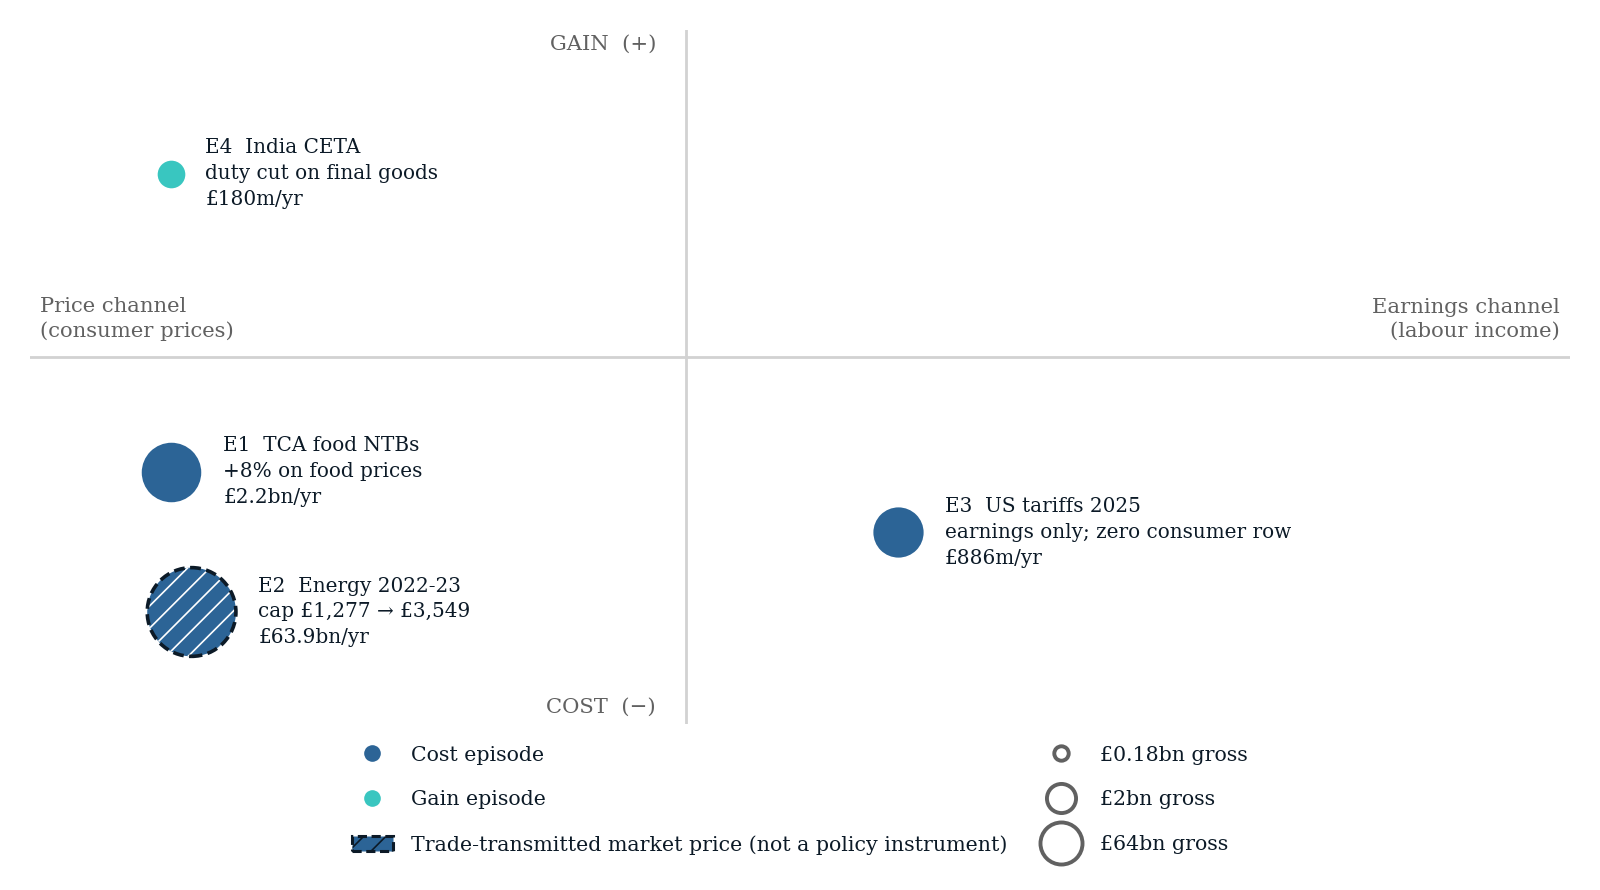
\includegraphics[width=0.9\textwidth]{figures/fig_episode_map.png}
\caption{The four episodes by channel and sign. Bubble area is log-scaled in shock size (energy: the counterfactual shock). Positions are classifications, not measurements.}
\label{fig:episode-map}
\end{figure}

\subsubsection{Episode 1: the TCA border (2021--23)}

The TCA took effect in January 2021,
replacing single-market membership with a border that is tariff-free
but carries non-tariff barriers. The price evidence is
quasi-experimental: exploiting cross-product variation in EU import
intensity, \citet{bakker2023} attribute roughly 8 percentage points of
the 25 per cent food-price rise between December 2019 and March 2023
to those barriers, a cumulative \pounds 250 per household on food
alone, \pounds 6.95 billion in aggregate (their household count;
\pounds 250 on the ONS count used here gives \pounds 7.1 billion),
with pass-through of barrier costs to consumers of 50--80 per cent and
the largest effects in high-EU-import products such as meat and dairy.
Their estimation window opens in December 2019, thirteen months before
the TCA took effect; the episode is dated 2021--23 here and the
pre-entry months enter as zeros. The March 2026 revision of the same
study, an unpublished working paper, raises the estimate to a 4 per
cent rise a year and 12 per cent over three years, with household
losses of \pounds 14.8 billion \citep[\pounds 536 per household;][]{bakker2026}. The paper stays on the 2023 estimate, whose
\pounds 250 cumulative anchors the headline path, so the level of the
food episode should be read as the lower of the two.

The identification is relative, across products, so economy-wide
effects may be missed. On the trade side, UK imports from the EU fell
about 25 per cent in relative terms on entry \citep{freeman2022}, and
in 2022 goods exports were an estimated \pounds 27 billion (6.4 per
cent) below counterfactual, with some 16,400 firms exiting EU
exporting entirely \citep{freeman2024}. The earnings side, by
contrast, rests on assumptions rather than estimates (the standing assumptions of the Office for Budget Responsibility
(OBR), a 15 per cent fall in trade intensity and a 4 per cent fall in
productivity; \citealp{obrbrexit}) and is not carried here.

% Generated by figures/make_figures.py -- do not edit by hand.
% Requires: \usepackage{booktabs}  (no other package needed)
% \rr = ragged-right inside a p{} cell, with \\ restored as the row
% terminator, so narrow columns neither overfull nor stretch-underfull.
\providecommand{\rr}{\raggedright\let\\\tabularnewline}

\begin{table}[tbp]
\centering
\footnotesize
\setlength{\tabcolsep}{3pt}
\renewcommand{\arraystretch}{1.15}
\caption{The four shocks: source and status}
\label{tab:first-stages}
\begin{tabular}{@{}p{1.75cm} p{1.70cm} p{1.45cm} p{2.30cm} p{2.10cm} p{2.75cm} p{1.85cm}@{}}
\toprule
\rr Episode & \rr Date & \rr Type & \rr Channel & \rr Source & \rr Key number & \rr Status \\
\midrule
\rr E1 TCA food non-tariff barriers & \rr Dec 2019--\newline Mar 2023$^{w}$ & \rr Policy & \rr Consumer prices (food) & \rr \citet{bakker2023} & \rr $+8$ pp on food prices & \rr Estimate\newline (ex post) \\[3pt]
\rr E2 Energy 2022--23 & \rr Apr 2022--\newline Mar 2023 & \rr Market & \rr Consumer prices (energy) & \rr \citet{ofgem2021, ofgem2022, ofgemcap2023}; \citet{obrenergy2023} & \rr FY-mean cap \pounds\SsBaseFyCap\ $\to$ \pounds\SsCounterFyCap\ (\pounds\SsRealisedFyCap\ with the Guarantee) & \rr Observed\newline (statutory) \\[3pt]
\rr E3 US tariffs 2025 & \rr 2025--26 & \rr Policy\newline (foreign) & \rr Earnings only; no UK retaliation & \rr Constructed here (Appendix~\ref{app:e3}) & \rr \pounds\MsUSTariffGrossShockMillions m/yr earnings loss (unit elasticity) & \rr Scenario\newline (assumed) \\[3pt]
\rr E4 UK--India agreement & \rr 2026-- & \rr Policy & \rr Consumer prices (clothing, footwear, food) & \rr \citet{dbtindia2026} & \rr \pounds180m/yr duty cut on final goods & \rr Projection\newline (ex ante) \\[3pt]
\bottomrule
\end{tabular}

\vspace{2pt}
\begin{minipage}{\linewidth}\footnotesize
\emph{Notes.} Type distinguishes a policy instrument from a
market price imported through the terms of trade. E3's consumer-price effect is exactly zero (the UK imposed no
retaliatory tariffs), so its household incidence runs through earnings alone.
$^{w}$~the \emph{estimation} window of the cited study; the TCA itself
entered into force in January 2021.
\end{minipage}
\end{table}


\subsubsection{Episode 2: the terms-of-trade shock (2022--23)}

The 2022 energy and import-price surge was, in the Bank of England's
description, a terms-of-trade shock of a size unseen since the
mid-1970s: the terms of trade deteriorated 6.2 per cent in the year to
2022Q3 \citep{onstot2023}, and import prices rose 20 per cent relative
to output prices over two years \citep{broadbent2022}. The energy
import bill roughly doubled to \pounds 117 billion in 2022
\citep{oeuk2023}, the increase of roughly \pounds 60 billion being a
transfer abroad of about 2.5 per cent of GDP (author's calculation),
and of the roughly 17 per cent CPI rise to 2022Q4 more than 70 per
cent (12.7 points) was imported \citep{dhingrapage2023}.

The household price vector is observed and policy-mediated. Ofgem's
cap on a typical annual bill rose from \pounds 1,277 (winter 2021--22)
to \pounds 1,971 (April 2022), \pounds 3,549 (October 2022) and
\pounds 4,279 (January 2023) \citep{ofgem2021, ofgem2022, ofgemcap2023}, and the
Energy Price Guarantee held it at \pounds 2,500 from
October 2022, at an ex-ante cost the OBR put at \pounds 27 billion
within \pounds 47 billion of price subsidies and \pounds 78 billion of
total energy support \citep{obrenergy2023}. \citet{levell2025} put
counterfactual no-policy welfare losses at 6 per cent of income on
average, with some households facing much larger losses. This is the
best-measured shock of the four, with independent official figures for
both the aggregate shock and the retail price vector and a published
decomposition of the cap. The paper therefore measures the shock
before policy and treats the Guarantee and the other legislated
instruments as responses to it, so that automatic and discretionary
cushioning can be separated.

\subsubsection{Episode 3: the US tariffs (2025--26)}

The April 2025 US schedule, before any mitigation, set a 10 per cent
baseline and 25 per cent on motor vehicles and steel
\citep{boempr2025}. Because
pass-through of US tariffs to US import prices is close to complete
\citep{amitireddingweinstein2019, fajgelbaumetal2020, cavalloetal2021},
the UK effect runs through export demand and earnings rather than UK
consumer prices; the UK had imposed no retaliatory tariffs as of
November 2026, so the consumer-price side of this episode is zero. The
earnings scenario is constructed here
(Section~\ref{sec:results-tariff}; Appendix~\ref{app:e3}), on the same
microdata and model version as the price episodes. Each Standard Industrial Classification (SIC) division's
employee wage bill falls by the tariff rate times the US-export share
of turnover times an export-demand elasticity times the wage-bill
incidence, with the elasticity and the incidence both set to one as a
benchmark, not an estimate. The resulting earnings loss is
\pounds\MsUSTariffGrossShockMillions\ million a year.

The external reference points are the OBR's March 2025 scenarios
\citep[import-demand elasticity 0.4; peak GDP effects of $-0.6$ to
$-1.0$ per cent;][]{obr2025} and the Bank of England's estimate of an
effective US tariff on UK goods of about 11 per cent at April 2025
\citep{boempr2025}. At the OBR's elasticity the loss falls to about
\pounds\EThreeObrLowWageGrossM\ million a year, while the cushioning
rate under wage cuts is \EThreeObrLowWageRatePct\ per cent and that under
displacement is unchanged by construction. Indirect channels (exchange rates,
trade diversion, the May 2025 UK--US Economic Prosperity Deal's own tariff changes)
are outside the scenario.

\subsubsection{Episode 4: the UK--India agreement (2026--)}

The UK--India Comprehensive Economic and Trade Agreement entered into
force on 15 July 2026. Its shock is taken from the government's impact
assessment \citep{dbtindia2026}: long-run GDP $+\pounds 4.8$ billion a
year ($+0.13$ per cent by 2040), real wages $+0.19$ per cent
($\approx\pounds 2.2$ billion) and, on a different clock, after tariff
staging of up to ten years, consumer duty reductions of \pounds 220
million a year, \pounds 180 million of it on final goods, concentrated
in clothing (\pounds 132 million), footwear (\pounds 13 million) and
food and beverages (\pounds 12 million). Two parameters are assumed
rather than estimated, following the assessment's own caveats:
preference utilisation (the duty figures assume 100 per cent on static
2022 trade) and consumer pass-through of the duty savings. Only the
consumer-price gains are carried; the exercise computes what the
government's central figures imply for households by decile, which the
assessment does not report and its regulatory scrutineer asked for
\citep{rpc2025}.

\subsection{Method for the published expenditure tables}\label{sec:method}

The first analysis applies each price shock to published expenditure
aggregates; the household-stage method is set out in
Section~\ref{sec:secondstage-method}. Shock sizes are taken from the
sources in Table~\ref{tab:first-stages} and not re-estimated.
Expenditure by category and income decile comes from the ONS Family
Spending workbooks \citep{onsfamilyspending, onsfamilyspending2026}; price-cap levels, benefit
rates and CPI outturns are official data; pass-through and preference
utilisation are assumed, with pass-through varied; and the incidence
arithmetic involves no estimation step.

\paragraph{Consumption incidence.} Each episode's price vector is
applied to the relevant categories of household expenditure by
equivalised-disposable-income decile, giving a burden or gain in
pounds a year and as a share of total spending. These are first-order
calculations at fixed baskets, in the sense of \citet{deaton1989} and
\citet{porto2006}. The food shock is anchored on the published
cumulative of \pounds 250 per household: a linear ramp to the
end-state price effect overshoots it by a factor of
\MsTcaCrossCheckRatio, so the headline path is rescaled to the
published figure (Section~\ref{sec:results}). The energy shock uses
the same price path as the household stage, and the Guarantee's share
of it is computable per decile from cap levels alone. Where a
published aggregate exists it is reported beside the computed one as a
check, not used to rescale it: the National Audit Office's outturn for
the Guarantee is the main example.

\paragraph{Indexation arithmetic.} For a single adult the paper
computes the shortfall of the Universal Credit standard allowance in
2022--23 against indexation to contemporaneous CPI, month by month,
and against a single April uprating at that month's inflation rate
(Appendix~\ref{sec:results-rulebook}). This is statutory arithmetic on
public parameters, for one benefit and one household type; the
household stage prices the same lag across the whole benefit system.

\paragraph{Data caveats.} The financial year ending (FYE) 2025 Family Spending workbook carries
an ONS correction notice affecting percentage standard errors, so no
sampling-uncertainty statement is made on the expenditure inputs. The
food and energy episodes use the FYE2022 workbook (April 2021 to March
2022), the last year before the energy shock, and the UK--India
agreement the FYE2025 workbook. The two sit either side of a change in
the ONS equivalence scale, so income levels are not comparable across
them, and episodes are compared as shares of spending. Pass-through
assumptions are reported as separate variants. Ranges are bounds
across assumptions, not confidence intervals, and the status of each
shock (estimate, observation, projection or scenario) is given in
Table~\ref{tab:first-stages}.

\section{Incidence on published expenditure tables}\label{sec:results}

\subsection{Four episodes compared}\label{sec:results-anatomy}

Table~\ref{tab:ms-anatomy} sets the four episodes side by side and
Figure~\ref{fig:incidence-profile} plots the three price profiles.
The two adverse price shocks are regressive and the price gain is
proportional, and the ordering follows the budget shares of the goods
affected (Figure~\ref{fig:budget-shares}): food takes
\MsTcaBudgetSharePctDecOne\ per cent of bottom-decile spending against
\MsTcaBudgetSharePctDecTen\ at the top and energy
\MsEnergyBudgetSharePctDecOne\ against \MsEnergyBudgetSharePctDecTen,
while clothing and footwear take similar shares in every decile. The
UK--India gains are under 0.02 per cent of spending in every decile,
two orders of magnitude below the energy shock and one below the food
shock.

The rows are not on one clock. The energy row is the cost of one
crisis year on the realised path, after the Guarantee; without it the
bottom decile would have faced \MsEnergyGrossPctSpendDecOne\ per cent
of spending and the top \MsEnergyGrossPctSpendDecTen. The food row
averages a cumulative effect over a 39-month window, and at its
end-state rate is more than three times as large. The tariff row has no
entry for spending because its incidence runs through earnings, and
the last column records how each shock was cushioned: the food shock
by no instrument, the energy shock by legislated support, and the
tariff scenario by the tax--benefit system without any decision.

\begin{table}[htbp]
\centering
\caption{Four episodes compared: incidence from published expenditure tables}
\label{tab:ms-anatomy}
\small
\begin{tabular}{llrrrl}
\toprule
Episode & Type, channel & Shock & \multicolumn{2}{c}{\% of spending} & Cushioning rate \\
\cmidrule(lr){4-5}
  & & (per year) & D1 & D10 & (of counterfactual) \\
\midrule
TCA food, 2021--23 & policy, prices & \pounds\MsTcaWindowAvgAggBn\,bn & \MsTcaWindowAvgPctSpendDecOne & \MsTcaWindowAvgPctSpendDecTen & none legislated$^{t}$ \\
Energy, 2022--23 & market, prices & \pounds\MsEnergyRealisedAggBn\,bn & \MsEnergyRealisedPctSpendDecOne & \MsEnergyRealisedPctSpendDecTen & \SsEpgRatePct--\SsDiscretionaryRatePct\%$^{i}$ \\
US tariffs, 2025--26 & policy, earnings & \pounds\MsUSTariffGrossShockMillions\,m & \multicolumn{2}{c}{zero$^{z}$} & \EThreeDispTaxBenRatePct--\EThreeWageTaxBenRatePct\%$^{m}$ \\
UK--India, 2026-- & policy, prices & \pounds\MsCetaTotalMillions\,m$^{g}$ & \MsCetaBottomPctSpend & \MsCetaTopPctSpend & --- \\
\bottomrule
\end{tabular}
\begin{minipage}{.94\textwidth}\footnotesize
\emph{Notes.} Deciles are of equivalised disposable income; entries
are first-order incidence at fixed baskets on realised paths. Energy
is the 2022--23 rise in the consumption-weighted mean cap
(\pounds\MsEnergyRealisedMeanCapFyTwentyOne\ to
\pounds\MsEnergyRealisedMeanCapFyTwentyTwo,
$+$\MsEnergyRealisedRisePct\ per cent); TCA is the published
cumulative averaged over its window, and reads
\MsTcaPctSpendDecOne\ against \MsTcaPctSpendDecTen\ per cent at the
end-state rate. Cushioning rates measure different things and are not
summable. Per-decile detail is in Table~\ref{tab:decile-full}.
$^{t}$~no instrument was legislated against this episode
(Section~\ref{sec:results-tca-ss}).
$^{i}$~share of the counterfactual shock (\pounds\SsCounterAggBn\,bn
on household records, \pounds\MsEnergyGrossAggBn\,bn on the published
tables) cushioned by the Guarantee alone (\SsEpgRatePct\ per cent on
either base), by energy-specific instruments
(\SsEnergySpecificRatePct) and by the full stack
(\SsDiscretionaryRatePct), the last two on household records
(Section~\ref{sec:results-secondstage}).
$^{m}$~share of the gross earnings loss offset by taxes and benefits,
displacement to wage cut (Section~\ref{sec:results-tariff}); the
cushioning rate $c^{Y}$, which also counts pension contributions that
cease, is \EThreeDispRatePct--\EThreeWageRatePct\ per cent.
$^{z}$~the UK did not retaliate, so there is no consumer-price shock.
$^{g}$~gain, not cost; the decile shares allocate the
\pounds\MsCetaAllocatedMillions\ million with published spending
detail.
\end{minipage}
\end{table}

\begin{figure}[tbp]\centering
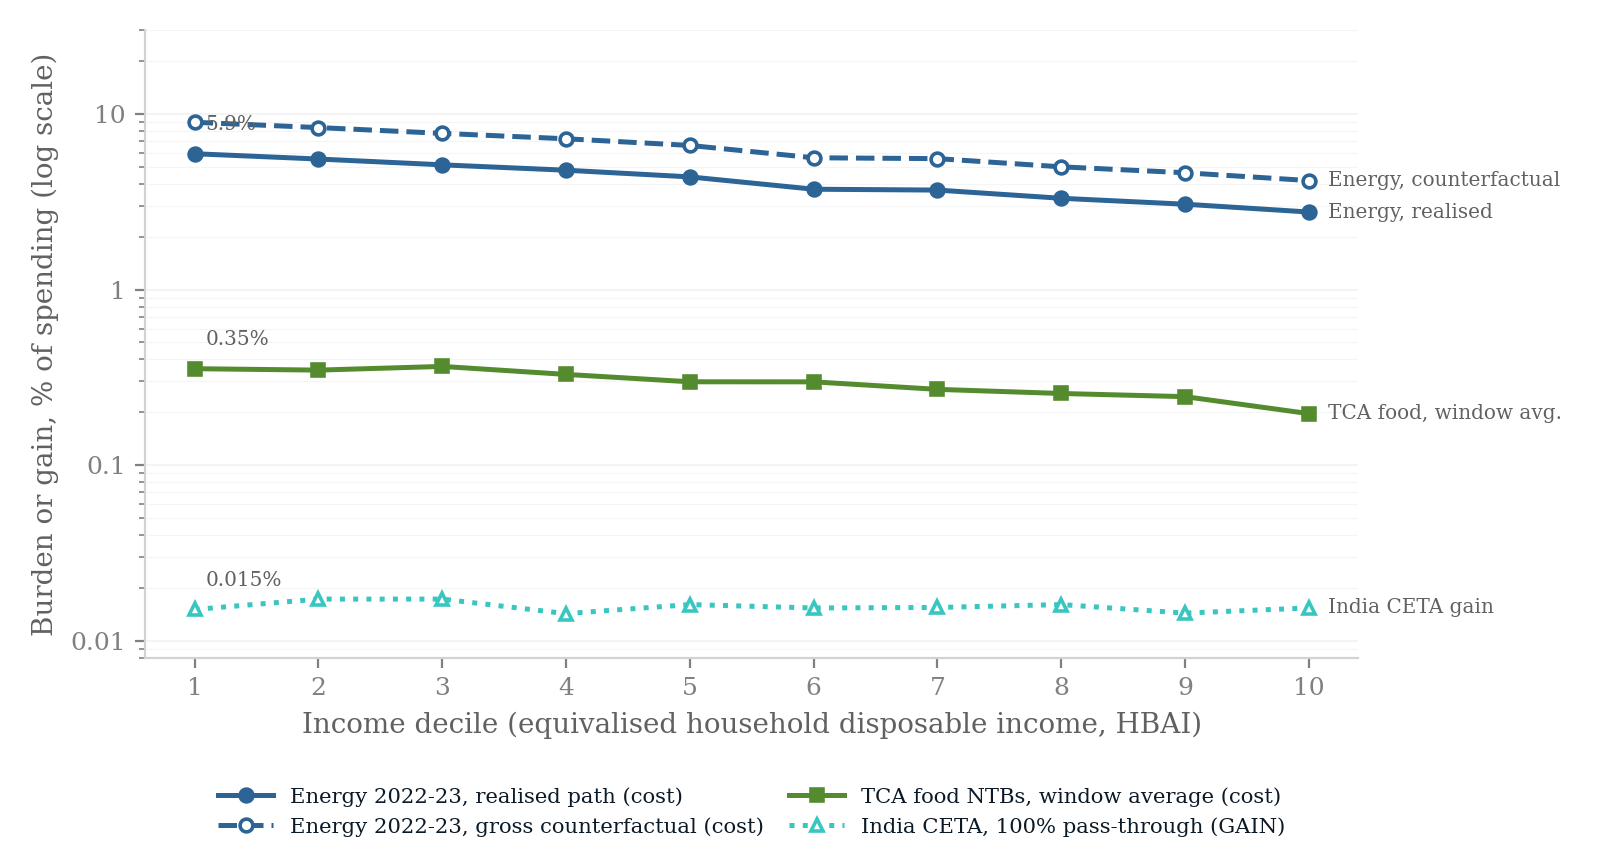
\includegraphics[width=\textwidth]{figures/fig_incidence_profile.png}
\caption{Incidence by income decile as a share of spending (log scale, magnitudes). Energy is shown realised (solid) and without the Energy Price Guarantee (dashed); the UK--India agreement is a gain (dotted).}
\label{fig:incidence-profile}
\end{figure}

\begin{figure}[tbp]\centering
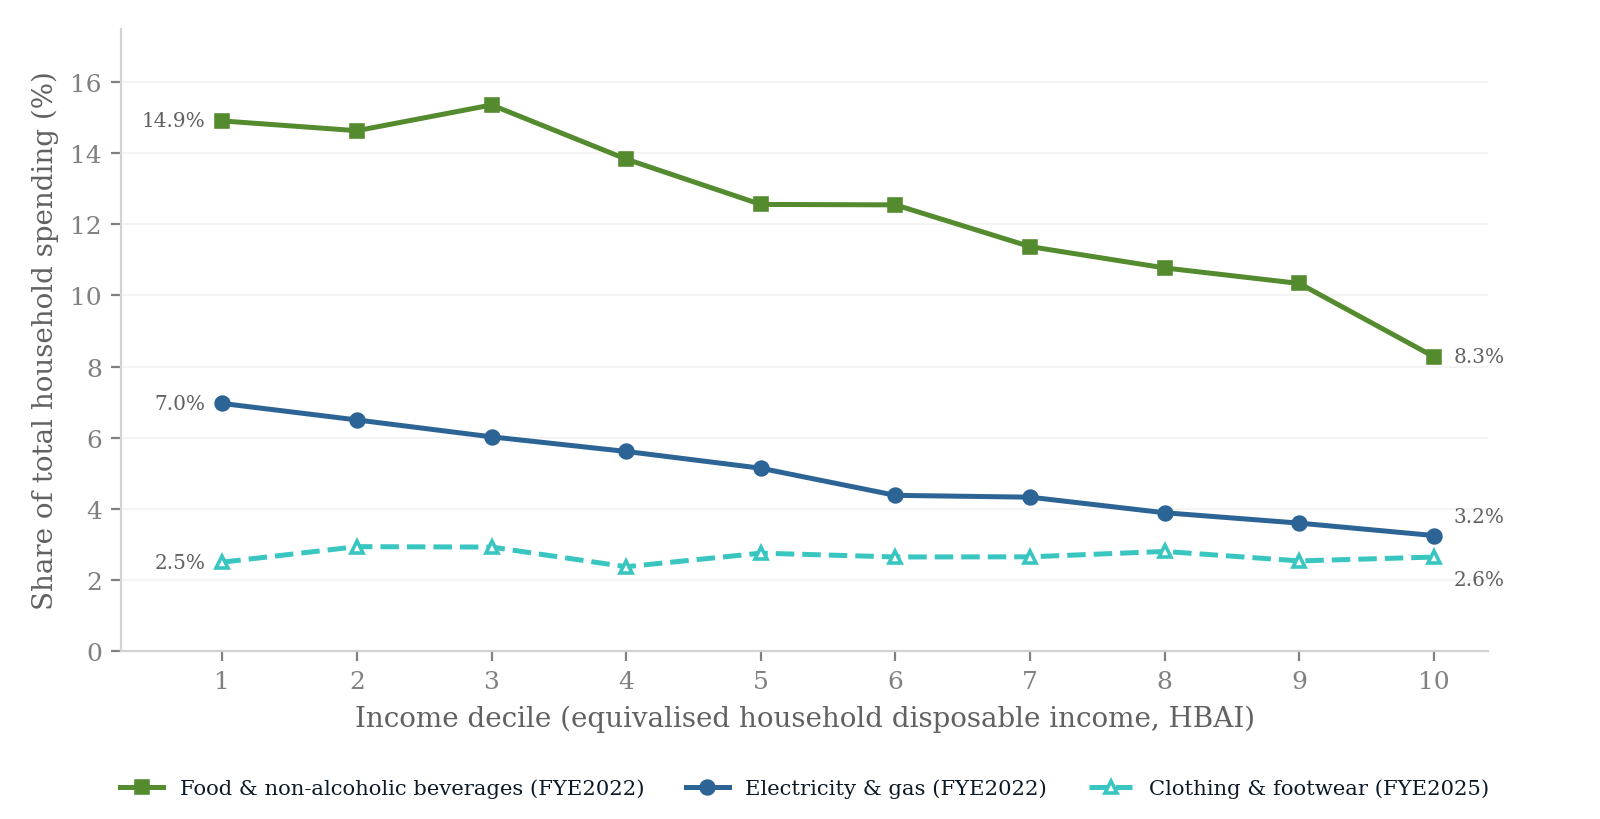
\includegraphics[width=\textwidth]{figures/fig_budget_shares.png}
\caption{Budget shares of the affected categories by income decile.}
\label{fig:budget-shares}
\end{figure}

\subsection{Episode detail}

\paragraph{TCA food prices.} The headline incidence uses the
window-average path implied by the published cumulative. The
\pounds\MsTcaPublishedCumulGbp-per-household figure implies an
average effect over the window of about 30 per cent of the 8 per cent
end-state: a linear ramp to the end-state would overshoot the
published figure by a factor of \MsTcaCrossCheckRatio, which is
consistent with a back-loaded price effect. This is an anchoring
choice, and the window-average path is obtained by rescaling to the
published cumulative. On that path the
shock costs \pounds\MsTcaWindowAvgGbpDecOne\ a year in the bottom
decile and \pounds\MsTcaWindowAvgGbpDecTen\ in the top,
\pounds\MsTcaWindowAvgAggBn\ billion in aggregate, and is regressive
as a share of spending (\MsTcaWindowAvgPctSpendDecOne\ against
\MsTcaWindowAvgPctSpendDecTen\ per cent), because food takes
\MsTcaBudgetSharePctDecOne\ per cent of bottom-decile spending against
\MsTcaBudgetSharePctDecTen\ at the top. The level is therefore the
published estimate's; this paper adds only its distribution across
deciles. The end-state figures are the unrescaled variant. They
overstate the burden over the estimation window, but they are the
continuing annual rate once the price effect is complete: on that
basis the shock is \pounds\MsTcaAggBnPerYear\ billion a year
(\pounds\MsTcaAnnGbpDecOne--\MsTcaAnnGbpDecTen\ a household;
\MsTcaPctSpendDecOne\ against \MsTcaPctSpendDecTen\ per cent of
spending).

\paragraph{The energy shock and the Guarantee.} Weighting each
quarter's cap by its share of annual consumption, households faced a
mean capped bill of \pounds\MsEnergyRealisedMeanCapFyTwentyTwo\ in
2022--23 (the \pounds 1{,}971 cap to September, the Guarantee's
\pounds 2{,}500 from October) against
\pounds\MsEnergyRealisedMeanCapFyTwentyOne\ the year before, a rise
of \MsEnergyRealisedRisePct\ per cent. It cost the bottom decile
\pounds\MsEnergyRealisedGbpDecOne\ a year,
\MsEnergyRealisedPctSpendDecOne\ per cent of its spending against
\MsEnergyRealisedPctSpendDecTen\ per cent at the top, and
\pounds\MsEnergyRealisedAggBn\ billion in aggregate. The
\emph{counterfactual shock} replaces the Guarantee with the caps Ofgem
set, \pounds\MsEnergyCapPeak\ for October to December and
\pounds 4{,}279 for January to March: a mean of
\pounds\SsCounterFyCap, $+$\MsEnergyGrossFactorPct\ per cent, which
would have cost the bottom decile \pounds\MsEnergyGrossGbpDecOne\ a
year, \MsEnergyGrossPctSpendDecOne\ per cent of its spending. The
Guarantee absorbed the difference, \pounds\MsEnergyCushionGbpDecOne\ a
year for a bottom-decile household and
\MsEnergyCushionShareFyPct\ per cent of the counterfactual shock in
every decile, because it capped a price. The
\pounds\MsEnergyCushionAggSixMonthsBn\ billion this implies compares
with an outturn of \pounds 24.0 billion \citep{nao2024}.

Three qualifications bound these numbers, and each is a different
kind of bound. The first is welfare against cash. The fixed-basket
figure is the first-order welfare measure, correct to a first
approximation by the envelope theorem, but households cut consumption,
so cash outlays rose by less. Applying the
\MsEnergyObservedDemandFallPct\ per cent weather-adjusted fall in
domestic gas consumption over the gas year to mid-May 2023
\citep{desnz2024} to the realised path gives a cash outlay of
\MsEnergyCashOutlayScalePct\ per cent of the fixed-basket figure (the
fall applies to the whole bill, not only its rise):
\pounds\MsEnergyCashOutlayGbpDecOne\ for the bottom decile and
\pounds\MsEnergyCashOutlayAggBn\ billion in aggregate. The gas
response is applied to the combined electricity and gas bill, and
electricity demand fell by less, so this slightly overstates the
reduction. The two figures answer different questions: what households
paid, and what they lost.

The second is how much of the shock is trade. On Ofgem's component
breakdown \citep{ofgem2021, ofgem2022}, wholesale energy accounts for
\MsEnergyWholesaleShareOfRisePct\ per cent of the cap's rise, so about
\pounds\MsEnergyRealisedTradeTransmittedAggBn\ billion of the realised
burden is exposure to a world-market-linked price
(Appendix~\ref{app:wholesale}, which also sets out why wholesale is
not the same as imported). The third is the price path, which is a
convention: holding the October cap through March, or weighting the
half-years equally rather than by consumption, lowers the
counterfactual shock and the Guarantee's share of it, to as little as
\SsEpgRateMinPct\ per cent
(Section~\ref{sec:results-sensitivity}).

Because the Guarantee capped a price, its cushioning rate is constant
across deciles by construction, and decile means understate the
dispersion it faced; \citet{levell2025} show that a price subsidy can
form part of an optimal package when income predicts exposure poorly.
Whether the overall discretionary response was progressive cannot be
judged from the Guarantee alone: the Energy Bills Support Scheme's
flat \pounds 400, the \pounds 150 Council Tax energy rebate and the
Cost of Living Payments, jointly of the same order as the Guarantee
and in part targeted, are not in the published-table analysis.
Section~\ref{sec:results-secondstage} adds them on household records.

\paragraph{The UK--India gains.} Of the \pounds\MsCetaTotalMillions\
million of final-goods duty reductions,
\pounds\MsCetaAllocatedMillions\ million falls in the three categories
with published spending detail and is allocated across deciles. At
full pass-through it is worth \pounds\MsCetaGainGbpPtHundredDecOne\ a
year to a bottom-decile household and
\pounds\MsCetaGainGbpPtHundredDecTen\ to a top-decile one
(\pounds\MsCetaGainGbpPtFiftyDecOne--\MsCetaGainGbpPtFiftyDecTen\ at
50 per cent). The gain is \MsCetaVerdict\ as a share of spending
(\MsCetaBottomPctSpend\ against \MsCetaTopPctSpend\ per cent),
though about three times larger in pounds at the top, and negligible
at any pass-through. The remainder of the final-goods
reductions falls in categories without published spending detail and
is not allocated.

\section{The household stage}\label{sec:results-secondstage}

\subsection{Method}\label{sec:secondstage-method}

The household stage uses PolicyEngine UK \citep{policyengineuk}, an
open-source static microsimulation model that encodes UK income tax,
National Insurance and the main benefits as dated statutory
parameters, in the tradition surveyed by \citet{figari2015}. It is run
through policyengine.py 6.20.0 (PolicyEngine UK
\SsPolicyEngineVersion) on the certified release of the Microcosm UK
2024--25 dataset \citep{microcosmuk}, a versioned build identified by
checksum. Its \SsHouseholdsRecords\ household records derive from the
Family Resources Survey \citep{frs}, with consumption imputed from the
Living Costs and Food Survey \citep[LCFS;][]{lcfs}, wealth from the
Wealth and Assets Survey and high incomes from HMRC's Survey of
Personal Incomes (sources documented in \citealt{microcosmuk}), and with calibrated weights. The records descend from
\DataSourceHouseholds\ survey households, the unit the bootstrap
resamples; \DataSyntheticWeightPct\ per cent of household weight sits
on \DataSyntheticRecords\ synthetic records built from the Survey of
Personal Incomes.

\runin{Price path.} The counterfactual and realised energy paths are
means of the quarterly caps weighted by the model's consumption
profile (\SsFyWeightAprSepPct\ per cent in April to September,
\SsFyWeightOctDecPct\ in October to December, \SsSeasShareJanMarPct\ in
January to March): \pounds\SsCounterFyCap\ without the Guarantee,
\pounds\SsRealisedFyCap\ with it, against \pounds\SsBaseFyCap\ in
2021--22. The counterfactual uses the caps Ofgem set for each quarter,
including the January 2023 cap that the Guarantee overrode. Both paths
use one basis: comparing a point-to-point cap ratio with a
financial-year mean would silently change the denominator of the
cushioning rate. Section~\ref{sec:results-sensitivity} reports three
alternative paths.

\runin{Rebasing.} The dataset's energy spending is at 2024--25 prices,
so its level reflects later prices while the distribution across
households reflects quantities. Its weighted mean is rebased to the 2021--22 mean cap, a factor of
\SsRebaseFactor, preserving each household's relative position. Shock
aggregates are linear in this factor and should be read as conditional
on it; the within-decile results are invariant to it. Cushioning rates are not: flat-cash instruments do
not scale with the rebase while the shock does, so the rates are
reported across rebase factors (Section~\ref{sec:results-sensitivity}).

\runin{Policy year and data year.} The episode is 2022--23; the
simulation scores it under 2023--24 rules, and under 2022--23 rules
for the uprating counterfactual, on households, weights and nominal
incomes held at 2024--25 values, so the microdata serve as a
distributional template for the episode. The instruments enter as
statutory cash amounts, the Cost of Living Payments computed per
benefit unit on the model's 2022--23 rules, so the discretionary
results are insensitive to the policy year. Deflating 2024--25 incomes to the policy year leaves the
full-stack rate at \SsDeflFullRatePct\ per cent and moves no decile by
more than \SsDeflMaxDecileDiffPp\ points, and excluding the synthetic
records gives \SsNoSynDiscretionaryRatePct\ per cent
(Appendix~\ref{app:conventions}). The tariff scenario runs on the same
records projected to 2026--27 with the model's uprating indices, under
2026--27 rules.

\runin{Instruments.} The Guarantee enters as the difference between
the two paths; the Energy Bills Support Scheme as \pounds 400 to every
household; the Council Tax energy rebate as \pounds 150 to households
in bands A to D in England, Scotland and Wales
(\pounds\SsCtrBn\ billion to \SsCtrHouseholdsM\ million households);
and the 2022--23 Cost of Living Payments on the model's eligibility
rules. The first three are \emph{energy-specific}; the \emph{full
stack} adds the Cost of Living Payments. The Warm Home Discount is not
modelled.

\runin{Deciles, shares and levels.} Deciles are of equivalised HBAI
before-housing-costs income, and burdens are shares of household
expenditure, with numerator and denominator rebased to 2021--22.
Household weights total \SsWeightedHouseholdsM\ million against an ONS
count of \SsOnsHouseholdsM\ million, so aggregates sit about
\SsWeightExcessPct\ per cent high; ratios are unaffected.

\runin{Accuracy.} The mismatches set out above, 2024--25 incomes and
weights for a 2022--23 episode, an FYE2022 spending base, household
weights above the ONS count and the gap between the household-stage
and published-table aggregates, mean that levels in this section are
indicative, with an error band that is not computed. Figures are
reported to three digits for reproducibility, not as claimed accuracy.
Appendix~\ref{app:conventions} gives each convention in full and
Appendix~\ref{app:recon} reconciles the aggregates.

\subsection{No within-year automatic response to a price shock}

Means-tested awards condition on nominal income, and non-means-tested
benefits are paid at rates fixed each April. A price shock leaves
nominal income untouched, so neither can respond within the year: the
zero is a property of the rules and of the fixed nominal inputs, not
an empirical finding. Running the model on baseline inputs and on
energy inputs shocked to the realised path, the change across the
fourteen modelled cash benefits is \pounds\SsAutomaticBn\ billion. The
model's own Energy Price Guarantee variable does read energy
consumption; the paper classifies the Guarantee as discretionary
(Appendix~\ref{app:native}).

Three qualifications bound the claim. It is a first-round statement: a
shock of this size moved wages and self-employment income in general
equilibrium, and those channels would trigger means-tested responses
that this calculation excludes. It is a statement about the modelled
system, so channels outside it, the Warm Home Discount, capital
drawdown altering means-tested entitlement and passported eligibility
shifting at the margin, could move the true figure off zero, though
all are small relative to the shock. And it is an in-year statement:
indexation is the system's automatic price-side channel, and it
arrives late rather than never. The result is consistent with
\citet{cohenfollette2000}, who find in a macro model that automatic
stabilisers do very little against a supply shock.

\subsection{Indexation arrives late}\label{sec:results-indexation}

Benefits rose 3.1 per cent in April 2022, indexed to the previous
September, against inflation over the year of about 10 per cent
\citep{cribb2023}, the benefit-erosion mechanism analysed across
countries by \citet{paulus2020}. I cost that gap as a parameters-only reform: on
the same households under 2022--23 rules, the \SsLagReformParameters\
uprated benefit parameters are raised by $1.101/1.031$, the uprating
that September 2022 inflation would have delivered. Benefit income
rises by \pounds\SsLagReformBn\ billion (\SsLagReformPctOfBase\ per
cent of the \pounds\SsLagReformBaseBn\ billion base), tapers and caps
included: \pounds\SsLagReformStatePensionBn\ billion on the state
pension and \pounds\SsLagReformNonStatePensionBn\ billion on other
benefits, of which \pounds\SsLagReformUcBn\ billion is Universal
Credit and \pounds\SsLagReformDisabilityCarerBn\ billion disability
and carer benefits. Pensioner benefit units gain
\pounds\SsLagReformPensionerBn\ billion and working-age units
\pounds\SsLagReformWorkingAgeBn\ billion, and household net income
rises by \pounds\SsLagReformNetIncomeBn\ billion once tax is taken
into account. Income-related Employment and Support Allowance and
Jobseeker's Allowance enter the data as reported amounts; scaling them
would add \pounds\SsLagReformReportedAddOnBn\ billion. The
counterfactual is a perfect-foresight benchmark, since the September
2022 rate was not known in April.

As a cross-check, scoring the same households under the 2022 and 2023
parameter systems moves the fourteen benefits from
\pounds\SsVinBenefitBaseRuleTwentyTwo\ to
\pounds\SsVinBenefitBaseRuleTwentyThree\ billion,
\pounds\SsVinPerPointBn\ billion per point of the April 2023 uprating,
or \pounds\SsVinLagCostBn\ billion at the reform's factor of
\SsLagReformParameterFactorPct\ per cent.
That difference also contains non-uprating changes (the benefit cap,
work allowances, childcare caps and the July 2022 National Insurance
threshold), which is why the parameters-only reform is the headline. Both sit above the roughly \pounds 12 billion real fall
of \citet{obrwelfare2022}, on a different base and counterfactual, and
below the \pounds\SsLagReformFlatBn\ billion of a flat
multiplication of the same base by that factor, because of tapers and caps. For a single adult on
Universal Credit the standard allowance fell
\pounds\MsUcLagCostFlatAltGbp\ short of a single April 2022 uprating
at that month's CPI inflation of 9.0 per cent, and
\pounds\MsUcLagCostGbp\ short of month-by-month indexation over the
year (Appendix~\ref{sec:results-rulebook}).

\begin{table}[tbp]
\centering
\caption{The April 2022 uprating shortfall and the Cost of Living Payments by income decile, pounds per household, 2022--23}
\label{tab:lagdecile}
\small
% generated by uprating_lag_reform.py -- do not edit by hand.
\begin{tabular}{lrrrr}
\toprule
Decile & Lag cost (\pounds) & \% of energy shock & CoL payments (\pounds) & CoL $-$ lag (\pounds) \\
\midrule
1 & 472 & 26.2 & 433 & $-$39 \\
2 & 737 & 39.2 & 474 & $-$263 \\
3 & 744 & 41.6 & 472 & $-$271 \\
4 & 769 & 40.7 & 447 & $-$322 \\
5 & 676 & 34.5 & 384 & $-$292 \\
6 & 572 & 29.6 & 314 & $-$258 \\
7 & 524 & 26.4 & 267 & $-$256 \\
8 & 370 & 18.0 & 174 & $-$195 \\
9 & 260 & 11.6 & 102 & $-$159 \\
10 & 228 & 8.9 & 94 & $-$134 \\
\midrule
All households & 535 & 26.6 & 316 & $-$219 \\
\bottomrule
\end{tabular}

\begin{minipage}{.8\textwidth}\footnotesize
\emph{Notes.} Lag cost is the rise in benefit income had the April
2022 uprating been 10.1 rather than 3.1 per cent, on 2022--23 rules.
The second column divides it by the decile's counterfactual energy
shock for scale only. CoL is the modelled Cost of Living Payments.
Differences are computed on unrounded values.
\end{minipage}
\end{table}

Table~\ref{tab:lagdecile} sets the shortfall by decile beside the Cost
of Living Payments. The shortfall averages \pounds\SsLagDecAllGbp\ a
household and the payments \pounds\SsLagDecAllColGbp, and the
shortfall exceeded the payments in all \SsLagDecNetNegativeCount\
deciles, narrowly in the bottom one
(payments less shortfall: \SsLagDecOneNetGbp\ pounds in the bottom
decile, \SsLagDecFourNetGbp\ in the fourth and \SsLagDecAllNetGbp\ on
average); \SsLagDecBottomHalfSharePct\ per cent of it
falls on the bottom half of the distribution.

The shortfall is not a share of the energy shock. Its numerator is the
erosion of benefit income by all inflation, and dividing it by one
commodity's counterfactual would attribute to energy what food,
services and rents also did. The table scales it by that shock,
\SsLagDecAllPctOfShock\ per cent on average, only to show its size.
What the comparison establishes is narrower: the one automatic
price-side channel delivered its April 2022 step below the inflation
of the year in which the shock landed, and the general payments
legislated that year did not make up the difference in any decile.

\subsection{The discretionary response by income decile}

Against a counterfactual shock of \pounds\SsCounterAggBn\ billion, the
Guarantee absorbed \pounds\SsEpgBn\ billion (\SsEpgRatePct\ per cent),
the Energy Bills Support Scheme \pounds\SsEbssBn\ billion and the
Council Tax energy rebate \pounds\SsCtrBn\ billion. These
energy-specific instruments returned \SsEnergySpecificRatePct\ per
cent of the shock, \SsGridPaperEbssDOne\ per cent in the bottom decile
and \SsGridPaperEbssDTen\ in the top; the gradient comes from the two
flat payments, which are worth \pounds 400 and \pounds 150 whatever
the bill. Adding the Cost of Living
Payments (\pounds\SsColBn\ billion in the model against
\pounds\SsColOutturnTotalBn\ billion in DWP management information,
\citealp{dwpcol}) takes the full stack to
\pounds\SsDiscretionaryBn\ billion, \SsDiscretionaryRatePct\ per cent.
The two attributions are reported separately because the Cost of
Living Payments were legislated against inflation in general:
dividing them by the energy shock alone over-attributes them to it.
Across the four price-path conventions the Guarantee's rate is
\SsEpgRateMinPct--\SsEpgRateMaxPct\ per cent, the energy-specific rate
\SsEnergySpecificRateMinPct--\SsEnergySpecificRateMaxPct\ and the
full-stack rate \SsFullRateMinPct--\SsFullRateMaxPct.

On either attribution the rate falls with income above the third
decile (on the energy-specific stack the sixth is fractionally above
the fifth). On the full stack it is \SsGridPaperFullDOne\ per cent in
the bottom decile, \SsCushionPctOneDpDecTwo\ in the second and
\SsGridPaperFullMaxDecilePct\ in the third, falling to
\SsSeasCwActualFullDTen\ per cent in the top. Flat payments are worth
more against a small bill, and the Cost of Living Payments concentrate
in the lower deciles, so adding the flat-cash instruments turns the
Guarantee's constant rate into one that declines with income.
Figure~\ref{fig:decomp} shows the same decomposition in pounds.

On the headline path and the full sample, only decile
\SsDecilesAboveHundredList\ is returned more than its counterfactual
energy cost (\SsGridPaperFullMaxDecilePct\ per cent), and only as a
point estimate; on the equal-half-year paths the bottom decile also
exceeds 100 (Table~\ref{tab:paths}), and without the synthetic
records \SsNoSynDecilesAboveHundred\ deciles do. A household bootstrap (\SsBootReps\ resamples clustered on
the source survey household, as urged by \citealp{goedeme2013}) puts
\SsRateLo--\SsRateHi\ per cent around the aggregate rate and
\SsCushionDecOneLo--\SsCushionDecOneHi\ around the bottom decile's,
and the net amount borne (negative where the household gained) has 95 per cent
intervals of $\SsNetLoDecOne$ to $\SsNetHiDecOne$, $\SsNetLoDecTwo$ to
$\SsNetHiDecTwo$, $\SsNetLoDecThree$ to $\SsNetHiDecThree$ and
$\SsNetLoDecFour$ to $\SsNetHiDecFour$ pounds a year in deciles one
to four, all spanning zero, against $\SsNetLoDecFive$ to
$\SsNetHiDecFive$ in the fifth. The result also depends on the
rebase: the highest decile rate falls to 100 per cent at a factor of
\SsGridMaxDecileRebaseAtHundred, against the paper's \SsRebaseFactor.
And it compares support with the energy cost alone, not with
inflation, against which the previous subsection shows these
households were not made whole. The intervals cover sampling over the
survey base only, not weight calibration or imputation error.

Three external checks leave the rates in place. The modelled Energy
Bills Support Scheme, \pounds\SsEbssBn\ billion, is within one per
cent of its \pounds\SsEbssOutturnBn\ billion outturn, and scaling to
the outturn gives a full-stack rate of \SsCalFullRatePct\ per cent.
The modelled Cost of Living Payments are \SsColOutturnTotalExcessPct\
per cent above the official total, with the means-tested payment
\SsColOutturnMtExcessPct\ per cent, the pensioner payment
\SsColOutturnPenExcessPct\ per cent and the disability payment
\SsColOutturnDisExcessPct\ per cent from their official figures;
scaling each to its figure gives \SsColOutturnCalFullRatePct\ per
cent. And the modelled rebate for England,
\pounds\SsCtrEnglandBn\ billion, compares with
\pounds\SsCtrOutturnEnglandBn\ billion paid by September 2022
\citep{dluhcctr}. Without the rebate the energy-specific and
full-stack rates are \SsNoCtrEnergySpecificRatePct\ and
\SsNoCtrDiscretionaryRatePct\ per cent. Appendix~\ref{sec:results-mpc}
aggregates the flows into first-round demand and welfare-weighted
quantities under assumed parameters.

\begin{figure}[tbp]\centering
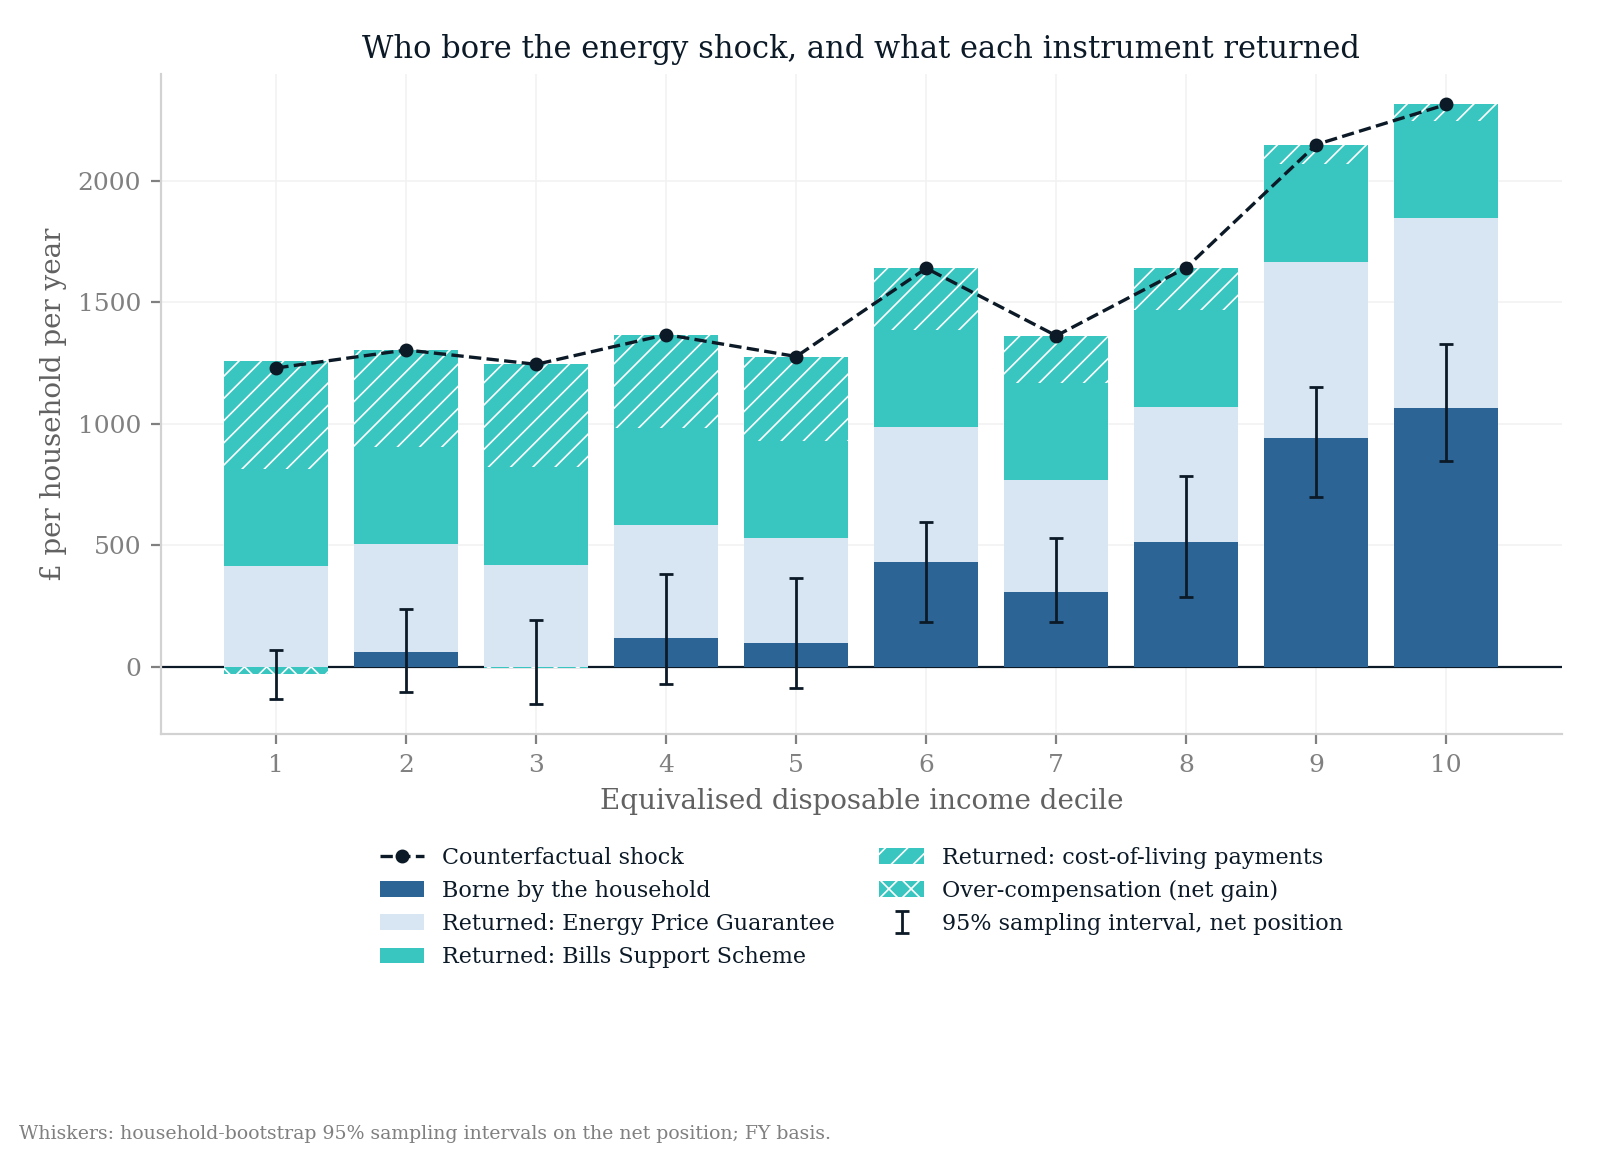
\includegraphics[width=\textwidth]{figures/fig_decomp.png}
\caption{Energy shock by decile, \pounds\ a year, split by instrument. Whiskers: 95 per cent bootstrap intervals on the net position.}
\label{fig:decomp}
\end{figure}

\subsection{Sensitivity to the rebase and the price path}\label{sec:results-sensitivity}

The headline rates depend on two conventions, the rebase factor and
the price path. Figure~\ref{fig:grid} varies the rebase factor from
0.55 to 1.05 and builds the stack up one instrument at a time;
Table~\ref{tab:grid} in Appendix~\ref{sec:results-grid} reports four
of those columns (\SsGridLowRebase\ to one). The Guarantee's rate does
not move with the rebase or across deciles, so the progressivity and
the rebase-sensitivity of the headline both come from the flat-cash
instruments. In every cell that includes a flat-cash instrument the
rate peaks in the third decile and is lower at the top than at the
bottom: with no rebase the full stack returns \SsGridUnityFullDOne\ per cent of the
bottom decile's loss against \SsGridUnityFullDTen\ per cent of the
top decile's, and \SsGridUnityFullRatePct\ per cent overall. The
number of deciles returned more than their cost is
\SsGridLowDecilesAboveHundred\ at a factor of \SsGridLowRebase, one at
the paper's and none at one. The paper's factor is computed, not
chosen, but it rests on the assumption that the dataset's mean bill
maps onto the mean cap; at that factor the Guarantee's
\pounds\SsEpgBn\ billion compares with an outturn of \pounds 24.0
billion.

The price path is the other convention. Table~\ref{tab:paths} reports
the four combinations of quarterly weights and final-quarter cap. The
headline, consumption weights with the caps Ofgem set, gives the
largest counterfactual shock and the highest Guarantee and
energy-specific rates; equal half-year weights with the October cap
held through March give the lowest. The Guarantee's absorption runs
from \pounds\SsEpgMinBn\ to \pounds\SsEpgMaxBn\ billion across the
four, either side of the \pounds 24.0 billion outturn, and its rate
from \SsEpgRateMinPct\ to \SsEpgRateMaxPct\ per cent. The flat-cash
instruments move the other way, since a smaller counterfactual shock
makes a fixed payment a larger share of it, so the full-stack rate
moves by only three points, and the bottom decile's from
\SsFullDOneMinPct\ to \SsFullDOneMaxPct\ per cent. The conclusions
that carry across all four are the ones the paper relies on: the
Guarantee absorbed between a third and a half of the counterfactual
shock, energy-specific support returned about two-thirds to seven-tenths, and
the full stack between \SsFullRateMinPct\ and \SsFullRateMaxPct\ per
cent, at rates that are highest in the lower deciles.

\begin{table}[tbp]
\centering
\caption{Energy cushioning rates under four price-path conventions}
\label{tab:paths}
\small\setlength{\tabcolsep}{4pt}
\begin{tabular}{lrrrrr}
\toprule
 & Shock & \multicolumn{4}{c}{Cushioning rate (\%)} \\
\cmidrule(lr){3-6}
Weights, final-quarter cap & (\pounds bn) & Guarantee & Energy-specific & Full stack & Full, D1 \\
\midrule
Consumption, actual (headline) & \SsSeasCwActualCounterAggBn & \SsSeasCwActualEpgRatePct & \SsSeasCwActualEbssRatePct & \SsSeasCwActualFullRatePct & \SsSeasCwActualFullDOne \\
Consumption, October held & \SsSeasCwHeldCounterAggBn & \SsSeasCwHeldEpgRatePct & \SsSeasCwHeldEbssRatePct & \SsSeasCwHeldFullRatePct & \SsSeasCwHeldFullDOne \\
Equal half-years, actual & \SsSeasEqActualCounterAggBn & \SsSeasEqActualEpgRatePct & \SsSeasEqActualEbssRatePct & \SsSeasEqActualFullRatePct & \SsSeasEqActualFullDOne \\
Equal half-years, October held & \SsSeasEqHeldCounterAggBn & \SsSeasEqHeldEpgRatePct & \SsSeasEqHeldEbssRatePct & \SsSeasEqHeldFullRatePct & \SsSeasEqHeldFullDOne \\
\bottomrule
\end{tabular}
\begin{minipage}{.94\textwidth}\footnotesize
\emph{Notes.} Actual: the caps Ofgem set, \pounds 3{,}549 for October
to December 2022 and \pounds 4{,}279 for January to March 2023. Held:
the October cap carried through March. Shock is the counterfactual shock. Each row uses its own rebase to
the 2021--22 mean cap. D1 is the bottom decile.
\end{minipage}
\end{table}

\begin{figure}[tbp]\centering
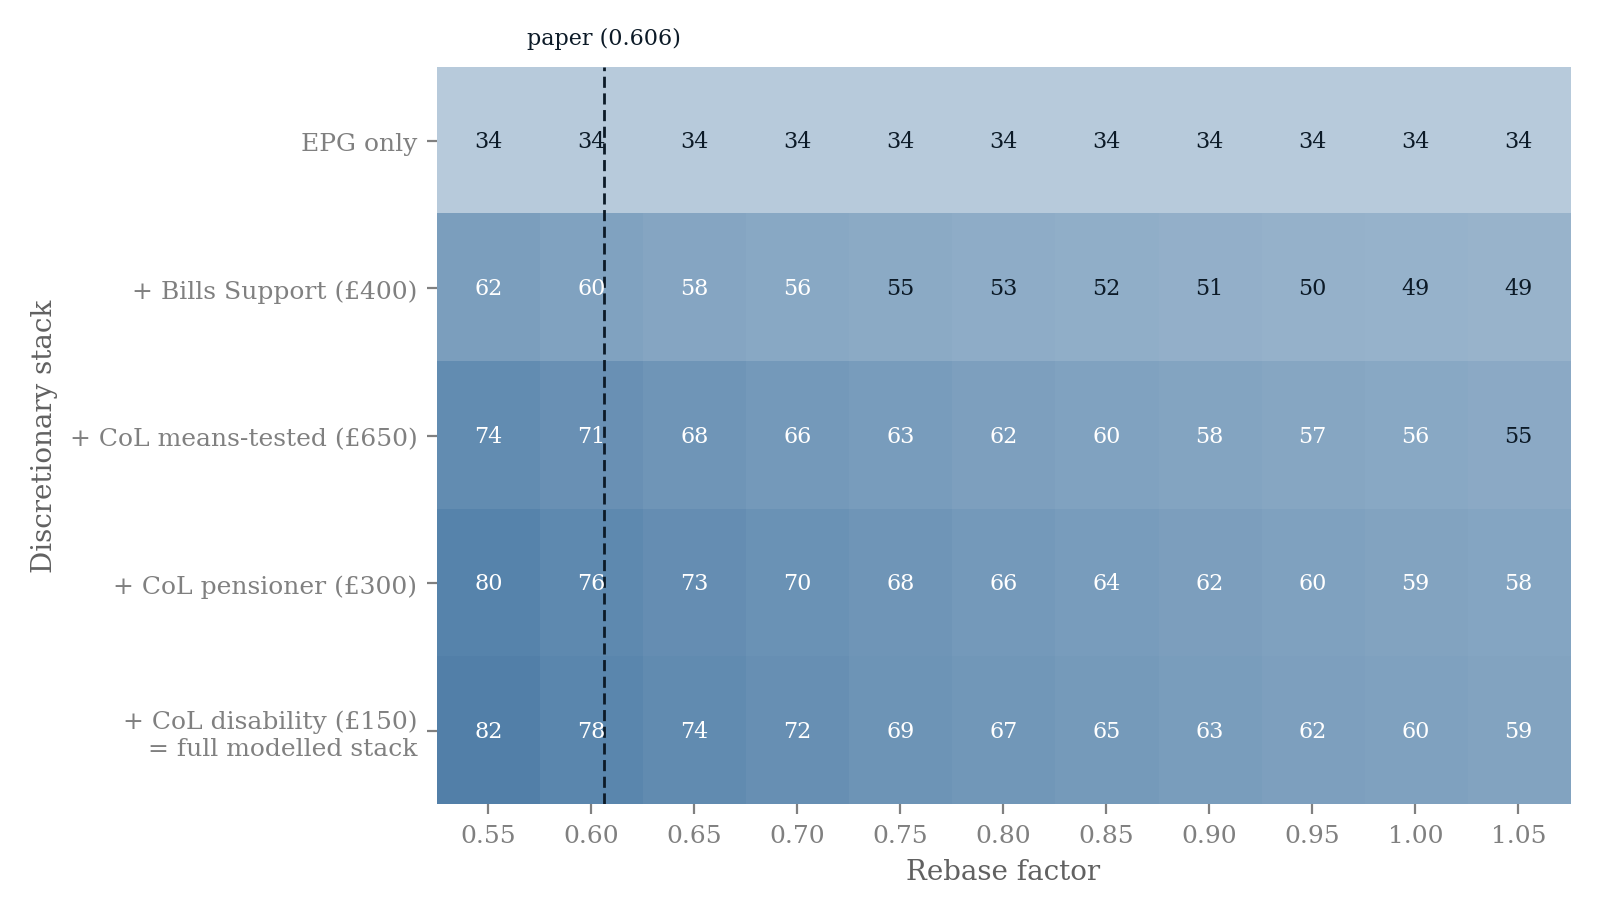
\includegraphics[width=0.85\textwidth]{figures/fig_grid.png}
\caption{Cushioning rate by rebase factor and instrument stack. Dashed box: the paper's rebase (\SsRebaseFactor); the colour scale saturates at 100 per cent.}
\label{fig:grid}
\end{figure}

\subsection{Imputed exposure varies mostly within deciles}\label{sec:results-withindec}

Figure~\ref{fig:within-decile} shows the realised burden by decile and
its spread within each. The burden runs from \SsBurdenPctSpendDecOne\
per cent of household expenditure in the bottom decile to
\SsBurdenPctSpendDecTen\ per cent in the top, against
\MsEnergyRealisedPctSpendDecOne\ and \MsEnergyRealisedPctSpendDecTen\
on the published tables; the gradient is regressive and close to
monotone. But it is a small part of the dispersion. A variance decomposition of the household burden puts
\SsBetweenPct\ per cent between deciles and \SsWithinPct\ per cent
within them (expenditure share, trimmed at the first and ninety-ninth
percentiles; bootstrap interval \SsWithinLo--\SsWithinHi\ for the
within-share). Untrimmed the within-share is
\SsWithinPctUntrimmed\ per cent, so trimming does not drive the
split, and in logs it is \SsWithinPctLog\ per cent. Within the bottom decile the burden runs from \SsPTenDecOne\ per
cent of spending at the tenth percentile to \SsPNinetyDecOne\ at the
ninetieth, a wider range than the gap between the bottom and top
decile means.

Two limits bound what this establishes. Exposure is imputed from LCFS donors, so part of this could be
donor-model variation. On the LCFS itself the within-decile share is
\SsLcfsWithinPct\ per cent in 2024--25 and \SsLcfsTwentyTwoWithinPct\
per cent in 2022--23, and the rebased decile burdens are close to
Microcosm's (Appendix Table~\ref{tab:lcfs}). The LCFS is the donor
survey, so this checks the gradient, not the level, which the rebase
removes: Microcosm's energy share is below the LCFS's in every decile; and its diary timing inflates within-decile
spread too; \citet{levell2025} use transaction data for this reason.
Excluding the synthetic records leaves the share at
\SsNoSynWithinPct\ per cent. Second, the quantity is the variance of
one commodity's expenditure share, not of welfare changes from trade
exposure on the earnings and expenditure sides, which is what
\citet{borusyakjaravel2024} decompose: the results point the same way
but are not the same quantity.

\begin{figure}[tbp]\centering
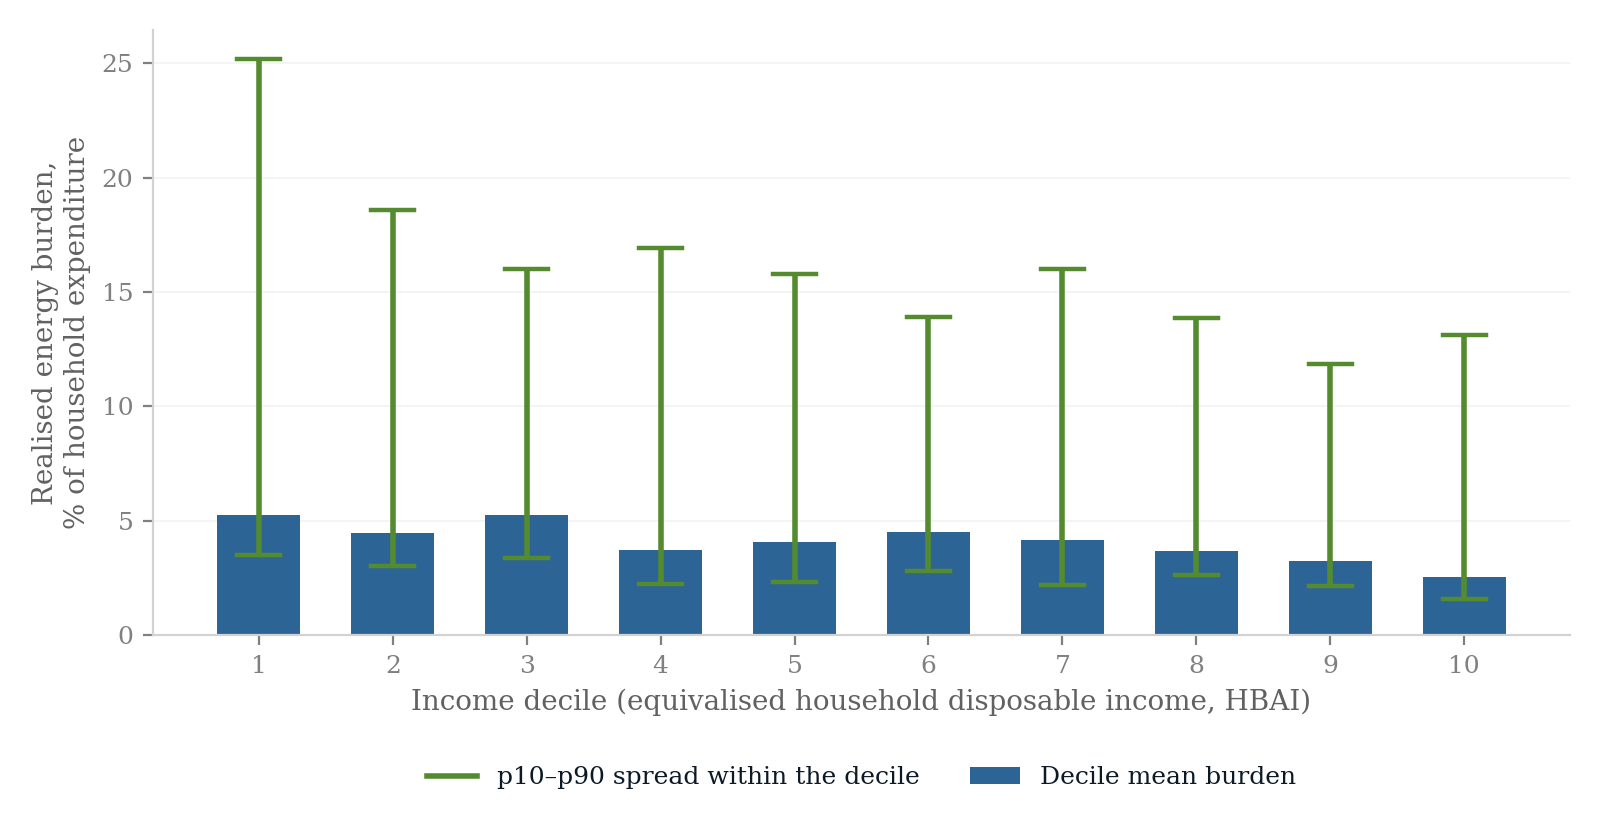
\includegraphics[width=\textwidth]{figures/fig_within_decile.png}
\caption{Realised energy burden by decile. Whiskers: 10th--90th percentiles of household burdens within the decile.}
\label{fig:within-decile}
\end{figure}

\subsection{The TCA food shock on household records}\label{sec:results-tca-ss}

The food shock (the window-average path of
Section~\ref{sec:results}) is priced against each household's imputed
food consumption on the same records, rebased to the ONS FYE2022
food-spending base (factor \SsTcaSsFoodRebase), the same convention as
the energy rebase. The aggregate, \pounds\SsTcaSsAggBn\ billion a
year, therefore matches the published-table figure
(\pounds\MsTcaWindowAvgAggBn\ billion) up to the \SsWeightExcessPct\
per cent excess in household weights; what is new is the
distribution. The burden is \SsTcaSsPctSpendDecOne\ per cent of
bottom-decile spending against \SsTcaSsPctSpendDecTen\ at the top
(\MsTcaWindowAvgPctSpendDecOne\ and \MsTcaWindowAvgPctSpendDecTen\ on
the published tables, close at the bottom and somewhat lower at the
top, a divergence of the consumption imputation), and larger in pounds
at the top, \pounds\SsTcaSsGbpDecOne\ against
\pounds\SsTcaSsGbpDecTen\ a year. \SsTcaSsWithinPct\ per cent of its
variance lies within deciles; within the bottom decile the burden runs
from \SsTcaSsPTenDecOne\ per cent of spending at the tenth percentile
to \SsTcaSsPNinetyDecOne\ at the ninetieth.

The cushioning side is short. No modelled entitlement reads food
consumption, so the within-year response is zero by construction.
Because the food shock built up over three upratings, annual
indexation did pick part of it up, with the lag described above. And
nothing was legislated against the food-price rise (general support
such as the Household Support Fund is outside the model). The Cost of Living Payments cushioned food-price inflation as
much as energy, so they cannot be counted for energy and ignored for
food; the comparison has to be between episode-specific instruments.
On that basis the state returned \SsEnergySpecificRatePct\ per cent
of the counterfactual energy shock and none of the food shock, which
had the same sign and a similar gradient across deciles. The contrast
does not depend on the energy conventions: the energy-specific rate is
between \SsEnergySpecificRateMinPct\ and \SsEnergySpecificRateMaxPct\
per cent on every price path, and above one half at every rebase
factor in Table~\ref{tab:grid}. The realised
energy shock was about \SsEnergyToTcaRatio\ times the size of the
window-average food shock, and faster; the paper does not estimate why
policymakers responded to one and not the other.

\subsection{The UK--India agreement on household records}\label{sec:results-ceta-ss}

The projected duty reductions are spread across households in
proportion to imputed spending on clothing, footwear and food. At full
pass-through the mean gain runs from \pounds\SsCetaSsGbpDecOne\ a year
in the bottom decile to \pounds\SsCetaSsGbpDecTen\ in the top
(\pounds\SsCetaSsGbpFiftyDecOne--\SsCetaSsGbpFiftyDecTen\ at 50 per
cent): \SsCetaSsPctSpendDecOne\ against \SsCetaSsPctSpendDecTen\ per
cent of spending. The gain is larger in pounds at the top,
near-proportional as a share of spending and small everywhere.
\SsCetaSsWithinPct\ per cent of its variance lies within deciles, the
pattern of the two adverse episodes: category spending, not income,
determines who is exposed, in either direction. There is no cushioning
side to compute, since gains trigger no statutory response.

\FloatBarrier
\subsection{The tariff scenario}\label{sec:results-tariff}

The scenario cuts the employee wage bill of
\EThreeIndDivisions\ SIC divisions by the tariff rate times the
US-export share of turnover, built from HMRC trade data and the ONS
Annual Business Survey \citep{hmrctrade, onsabs}
(Table~\ref{tab:e3-industry}). It reaches
\EThreeIndEmployeesM\ million employees with an employee-weighted mean
shock of \EThreeIndMeanShockPct\ per cent; motor vehicles carry
\EThreeIndTopLossSharePct\ per cent of the
\pounds\MsUSTariffGrossShockMillions\ million loss and the three
largest divisions \EThreeIndTopThreeLossSharePct\ per cent. The loss
is delivered either as a proportional wage cut to every employee in a
division or as displacement, each employee losing the job for a year
with probability equal to the shock; the displacement result is an
exact expectation over those independent job losses, computed from all
\EThreeDispExposedRecords\ exposed records.

\begin{table}[tbp]
\centering
\caption{Tariff scenario: exposure and earnings loss by industry}
\label{tab:e3-industry}
% Generated by analysis/e3_industry_table.py -- do not edit.
{\footnotesize
\begin{tabular}{@{}rlrrrrrrr@{}}
\toprule
SIC & Division & Tariff & US share & Shock & Employees & Mean pay & Loss & Share \\
 & & (\%) & (\%) & (\%) & (000) & (\pounds 000) & (\pounds m) & (\%) \\
\midrule
29 & Motor vehicles & 25 & 11.0 & 2.74 & 190 & 41.1 & 214 & 21.3 \\
28 & Machinery and equipment & 10 & 18.0 & 1.80 & 141 & 54.2 & 138 & 13.7 \\
26 & Computer, electronic, optical & 10 & 17.9 & 1.79 & 93 & 69.3 & 115 & 11.4 \\
30 & Other transport (incl. aerospace) & 10 & 15.7 & 1.57 & 140 & 48.8 & 108 & 10.7 \\
21 & Pharmaceuticals & 10 & 13.0 & 1.30 & 133 & 52.6 & 91 & 9.0 \\
32 & Other manufacturing & 10 & 13.9 & 1.39 & 134 & 40.8 & 76 & 7.6 \\
24 & Basic metals (incl. steel) & 25 & 5.1 & 1.26 & 79 & 54.9 & 55 & 5.4 \\
27 & Electrical equipment & 10 & 12.6 & 1.26 & 70 & 41.5 & 37 & 3.6 \\
14 & Wearing apparel & 10 & 14.6 & 1.47 & 48 & 48.4 & 34 & 3.4 \\
25 & Fabricated metal products & 10 & 3.1 & 0.31 & 212 & 50.1 & 33 & 3.2 \\
20 & Chemicals & 10 & 12.5 & 1.25 & 61 & 42.0 & 32 & 3.2 \\
11 & Beverages & 10 & 6.3 & 0.63 & 44 & 51.3 & 14 & 1.4 \\
 & Other 11 divisions & 10 & 2.0 & 0.20 & 812 & 38.2 & 61 & 6.1 \\
\midrule
 & All 23 exposed divisions & 12 & 8.1 & 0.98 & 2,158 & 45.0 & 1,007 & 100.0 \\
\bottomrule
\end{tabular}}

\begin{minipage}{.94\textwidth}\footnotesize
\emph{Notes.} US share is exports to the US over turnover; the shock
is the tariff rate times the US share, the proportional fall in the
division's employee wage bill. Employees, mean pay and loss are from
the household records at 2026--27 values. The \EThreeIndRowsShown\
largest divisions by loss are shown.
\end{minipage}
\end{table}

Taxes and benefits offset \EThreeWageTaxBenRatePct\ per cent of the
loss under wage cuts and \EThreeDispTaxBenRatePct\ per cent under
displacement. Counting the employee pension contributions that cease,
which HBAI income deducts, the cushioning rates are
\EThreeWageRatePct\ and \EThreeDispRatePct\ per cent (sampling
standard error \EThreeDispSamplingSe\ points on the latter).
Displacement is cushioned less than a wage cut, the reverse of the
EU-average ordering in \citet{dolls2012}. The gap is income tax: it
relieves \EThreeWageTaxOfGrossPct\ per cent of the loss under the wage
cut, at the worker's marginal rate, against \EThreeDispTaxOfGrossPct\
per cent under displacement, at the lower average rate, because the
personal allowance is forgone too. National Insurance relieves about
the same in both (\EThreeWageNiOfGrossPct\ and
\EThreeDispNiOfGrossPct\ per cent), and Universal Credit
(\EThreeDispUcOfGrossPct\ against \EThreeWageUcOfGrossPct) and the
flat-rate New Style Jobseeker's Allowance
(\EThreeDispJsaContribOfGrossPct) narrow the gap; the EU systems in
\citet{dolls2012} cushion unemployment more largely through
earnings-related insurance, which the New Style allowance is not
(Appendix Table~\ref{tab:e3-split}).

The displacement cushioning rate (\EThreeDispRatePct\ per cent) moves
as expected under the assumptions behind it. It is
\EThreeDispNoJsaRatePct\ per cent without
the New Style allowance and \EThreeSensJsaThirteenRatePct\ with 13
weeks of it; \EThreeSensTakeupLowRatePct\ and
\EThreeSensTakeupHighRatePct\ per cent with Universal Credit take-up
of \EThreeSensTakeupLow\ and \EThreeSensTakeupHigh\ in place of 0.8;
and higher, about \EThreeSensSixMonthAnnualRatePct\ and
\EThreeSensThreeMonthAnnualRatePct\ per cent, for spells of six and
three months, because income tax is then relieved at marginal rates.
The income-tax relief depends on how well paid the exposed workers
are. Their mean pay, weighted by expected displacement, is
\pounds\EThreeAsheModelMeanK\ thousand,
\EThreeAsheModelOverAsheMeanPct\ per cent of the ASHE mean for the
same divisions \citep{ashe}, and \EThreeHigherRateSharePct\ per cent
of them are above the higher-rate threshold against about
\EThreeAsheHigherRateSharePct\ per cent implied by ASHE, so the
relief is not inflated by overstated pay. The Exchequer cost (including employer contributions) is
\pounds\EThreeWageExchequerM\ million under wage cuts and
\pounds\EThreeDispExchequerM\ million under displacement, and poverty
before housing costs rises by \EThreeDispPovertyPp\ points under
displacement (Appendix~\ref{app:e3}).

These rates are not specific to the tariff. The same
\pounds\EThreeUnifGrossM\ million spread across all employees in
proportion to earnings is cushioned at \EThreeUnifWageRatePct\ per
cent as a wage cut and \EThreeUnifDispRatePct\ per cent as
displacement, within a point of the tariff pattern and about one
standard error: the rate is a property of the UK system applied to an
employee-earnings loss, not of the tariff's sector mix. Nor does it
depend on the scale of the loss: at the OBR's elasticity of 0.4 the
loss is \pounds\EThreeObrLowWageGrossM\ million and the rates are
\EThreeObrLowWageRatePct\ and \EThreeObrLowDispRatePct\ per cent, so
later mitigation of the schedule would change the size and sector mix
of the loss, not the rate at which it is cushioned.

Who bears it differs from the price shocks. Across household-weighted deciles of equivalised
HBAI income (Table~\ref{tab:e3-decile}), the loss is close to zero in
the bottom decile, \EThreeDispSharePctDecOne\ per cent of household
income and \EThreeLossSharePctDecOne\ per cent of the total, and
largest in the fourth and the eighth to tenth deciles
(\EThreeDispSharePctDecFour, and \EThreeDispSharePctDecTen\ to
\EThreeDispSharePctDecNine\ per cent); net of the cushion it is
\EThreeDispNetSharePctDecOne\ per cent in the bottom decile and
\EThreeDispNetSharePctDecTen\ in the top. In pounds per person a year
the net income loss rises from \pounds\EThreeDispDecGbpOne\ in the bottom decile
through \pounds\EThreeDispDecGbpFive\ in the fifth to
\pounds\EThreeDispDecGbpTen\ in the top (person-weighted deciles;
\pounds\EThreeDispDecGbpTwo, \EThreeDispDecGbpThree,
\EThreeDispDecGbpFour, \EThreeDispDecGbpSix, \EThreeDispDecGbpSeven,
\EThreeDispDecGbpEight\ and \EThreeDispDecGbpNine\ in the others).
Against the uniform benchmark the tariff pattern is lighter in the
bottom and top deciles; the excess in the fourth decile rests on few
records. Decile cells
rest on few effective records, so differences between adjacent deciles
are imprecise and the pattern should be read by broad group: almost
nothing at the bottom, most in the middle and at the top. Measured
like the price shocks, as a share of spending, the net loss is
\EThreeDispNetSpendSharePctDecOne\ per cent in the bottom decile and
\EThreeDispNetSpendSharePctDecTen\ in the top: the earnings shock
falls on the middle and top of the distribution, where the price
shocks fell on the bottom, though it is far smaller.

\begin{table}[tbp]
\centering
\caption{Tariff scenario: loss by income decile under displacement, per cent of household income}
\label{tab:e3-decile}
\small
\begin{tabular}{lrrrrr}
\toprule
 & \multicolumn{3}{c}{Tariff pattern} & \multicolumn{2}{c}{Uniform benchmark} \\
\cmidrule(lr){2-4}\cmidrule(lr){5-6}
Decile & Gross & Net & Share of loss & Gross & Net \\
\midrule
1 & \EThreeDispSharePctDecOne & \EThreeDispNetSharePctDecOne & \EThreeLossSharePctDecOne & \EThreeUnifDispSharePctDecOne & \EThreeUnifDispNetSharePctDecOne \\
2 & \EThreeDispSharePctDecTwo & \EThreeDispNetSharePctDecTwo & \EThreeLossSharePctDecTwo & \EThreeUnifDispSharePctDecTwo & \EThreeUnifDispNetSharePctDecTwo \\
3 & \EThreeDispSharePctDecThree & \EThreeDispNetSharePctDecThree & \EThreeLossSharePctDecThree & \EThreeUnifDispSharePctDecThree & \EThreeUnifDispNetSharePctDecThree \\
4 & \EThreeDispSharePctDecFour & \EThreeDispNetSharePctDecFour & \EThreeLossSharePctDecFour & \EThreeUnifDispSharePctDecFour & \EThreeUnifDispNetSharePctDecFour \\
5 & \EThreeDispSharePctDecFive & \EThreeDispNetSharePctDecFive & \EThreeLossSharePctDecFive & \EThreeUnifDispSharePctDecFive & \EThreeUnifDispNetSharePctDecFive \\
6 & \EThreeDispSharePctDecSix & \EThreeDispNetSharePctDecSix & \EThreeLossSharePctDecSix & \EThreeUnifDispSharePctDecSix & \EThreeUnifDispNetSharePctDecSix \\
7 & \EThreeDispSharePctDecSeven & \EThreeDispNetSharePctDecSeven & \EThreeLossSharePctDecSeven & \EThreeUnifDispSharePctDecSeven & \EThreeUnifDispNetSharePctDecSeven \\
8 & \EThreeDispSharePctDecEight & \EThreeDispNetSharePctDecEight & \EThreeLossSharePctDecEight & \EThreeUnifDispSharePctDecEight & \EThreeUnifDispNetSharePctDecEight \\
9 & \EThreeDispSharePctDecNine & \EThreeDispNetSharePctDecNine & \EThreeLossSharePctDecNine & \EThreeUnifDispSharePctDecNine & \EThreeUnifDispNetSharePctDecNine \\
10 & \EThreeDispSharePctDecTen & \EThreeDispNetSharePctDecTen & \EThreeLossSharePctDecTen & \EThreeUnifDispSharePctDecTen & \EThreeUnifDispNetSharePctDecTen \\
\midrule
All & \EThreeDispSharePctDecAll & \EThreeDispNetSharePctDecAll & \EThreeLossSharePctDecAll & \EThreeUnifDispSharePctDecAll & \EThreeUnifDispNetSharePctDecAll \\
\bottomrule
\end{tabular}
\begin{minipage}{.8\textwidth}\footnotesize
\emph{Notes.} Gross is the earnings loss and net the fall in household
net income, each over the decile's household net income. Share of loss
is the decile's share of the gross earnings loss, per cent.
\end{minipage}
\end{table}


\FloatBarrier
\section{Conclusion}\label{sec:discussion}

The UK's tax--benefit system cushions earnings losses automatically
and price rises only with a lag. In the tariff scenario taxes and
benefits offset \EThreeDispTaxBenRatePct\ to \EThreeWageTaxBenRatePct\
per cent of the lost earnings, at a rate that
would apply to any employee-earnings loss of that size; and, like the
same loss spread across all employees, it falls mainly on households
in the middle and top of the distribution rather than the bottom. Against the two price shocks the system paid nothing within
the year, and its one automatic channel, indexation, delivered the
April 2022 uprating below that year's inflation, a shortfall larger
than the Cost of Living Payments in every income decile.

Both adverse price shocks were regressive because they fell on food
and energy, and the price gain from the UK--India agreement is flat
because it falls on clothing and footwear: which goods a shock hits,
not only how large it is, determines who bears it. But decile means
are a small part of the picture. \SsWithinPct\ per cent of the
variance in the energy burden lies within income deciles, the pattern
from which \citet{levell2025} conclude that instruments conditioned on
income target energy exposure poorly.

The results carry limitations. Three shocks are taken from published
sources with their own identification and the fourth is assumed; the
incidence is first-order and static; the price and earnings channels
are not combined on the same households; household energy and food
spending are imputed; the decomposition counts all legislated support
as discretionary; and the energy levels depend on the price-path and
rebasing conventions, which is why the paper reports ranges. The
sampling intervals reported cover the survey base only, and are
narrower than these modelling approximations.
Natural extensions are to combine the two channels on the same
households and to replace fixed-weight indices with the non-homothetic
cost-of-living indices of \citet{hochmuth2025}.

What filled the gap on the price side was discretion, and it was
applied to one shock and not the other. The energy shock was met with
instruments that returned \SsEnergySpecificRatePct\ per cent of its
counterfactual cost
(\SsEnergySpecificRateMinPct--\SsEnergySpecificRateMaxPct\ across
price-path conventions), or \SsDiscretionaryRatePct\ per cent
(\SsFullRateMinPct--\SsFullRateMaxPct) with the Cost of Living
Payments, at rates that fall with income above the third
decile and reach the full cost near the bottom of the distribution
once general support is counted. The post-Brexit food-price rise, of
the same sign and with a similar gradient across deciles, was met with
none. The two differed in size and speed, and the paper does not
estimate why the responses differed.
\label{sec:mainend}

\subsection{Limitations and future work}\label{sec:roadmap}

Three extensions follow directly. First, the consumption and earnings
channels of an episode could be combined on common households, so
that their incidence is compared household by household rather than
distribution by distribution. Second, the three-way decomposition of
Section~\ref{sec:framework} (the rules as they stood, the preceding
year's rules, and the discretionary layer switched off) could be
computed for every episode rather than for energy alone; the microdata
carry inputs for a single year, so earlier rule years are applied to
later households, and the reconciliation of the uprating-lag figure
with the OBR's belongs here. Third, the fixed-weight decile indices
could be replaced by the non-homothetic distributional cost-of-living
indices of \citet{hochmuth2025}, which need only aggregate prices,
expenditure shares and a cross-sectional expenditure distribution. Two
limits would survive these extensions. The consumption imputation
carries its own error, inherited from the LCFS donor sample, and error
correlated with benefit status would bias the covariance between
exposure and cushioning; a validation of the imputed within-decile
spread against the donor sample is the first check to add. And the
rulebook decomposition attributes to ``discretion'' whatever was
legislated, which bundles shock response with policy that would have
happened anyway: a labelling choice, not an identification claim. One
further limit is specific to the data year: 2024--25 nominal incomes
are evaluated under earlier rules without deflation, so means-tested
entitlement under the 2022--23 and 2023--24 rules may be slightly
understated.

\section*{Data and code availability}

The replication code, the pinned public inputs and the generated
results are at \url{https://github.com/PolicyEngine/uk-trade-shock-study}.
The decile-table analysis uses only public data (ONS Family Spending
workbooks, Ofgem price-cap documents, DWP benefit rates and the ONS
consumer prices index). The household-level analysis uses the
certified Microcosm UK 2024--25 dataset through policyengine.py 6.20.0
(PolicyEngine UK \SsPolicyEngineVersion). That dataset is derived from
the Family Resources Survey, which is licensed through the UK Data
Service, so it cannot be redistributed with the code; access is
through PolicyEngine's data repository under the same licence. The
repository's notes record the dataset build identifier and checksum.

\section*{Competing interests}

The author is a Research Associate at PolicyEngine, the non-profit
organisation that develops the microsimulation model and dataset used
in this paper. The research received no external funding.


\begingroup\sloppy
\begin{thebibliography}{99}

\bibitem[Alabrese et~al.(2026)]{alabrese2026}
Alabrese, E., Edenhofer, J., Fetzer, T. and Wang, S. (2026).
\newblock Measuring the regional economic cost of Brexit: Evidence as of 2026.
\newblock CAGE Working Paper No.~486 (revised June 2026), University of Warwick.

\bibitem[Amaglobeli et~al.(2026)]{amaglobeli2026}
Amaglobeli, D., Black, S., Celasun, O. and Toscani, F. (2026).
\newblock Europe's second energy shock: Avoiding the mistakes of 2022.
\newblock \emph{Intereconomics}, 61(3), 189--190. \doi{10.2478/ie-2026-0035}.

\bibitem[Amiti et~al.(2019)]{amitireddingweinstein2019}
Amiti, M., Redding, S.~J. and Weinstein, D.~E. (2019).
\newblock The impact of the 2018 tariffs on prices and welfare.
\newblock \emph{Journal of Economic Perspectives}, 33(4), 187--210.

\bibitem[Amores et~al.(2025)]{amores2025}
Amores, A.~F., Basso, H.~S., Bischl, J.~S., De~Agostini, P., De~Poli, S., Dicarlo, E., Flevotomou, M., Freier, M., Maier, S., Garc\'ia-Miralles, E., Pidkuyko, M., Ricci, M. and Riscado, S. (2025).
\newblock Inflation, fiscal policy, and inequality: The impact of the post-pandemic price surge and fiscal measures on European households.
\newblock \emph{Review of Income and Wealth}, 71(1), e12713. Earlier: ECB Occasional Paper 330 (2023).

\bibitem[Ari et~al.(2022)]{ari2022}
Ari, A., Arregui, N., Black, S., Celasun, O., Iakova, D., Mineshima, A., Mylonas, V., Parry, I., Teodoru, I. and Zhunussova, K. (2022).
\newblock Surging energy prices in Europe in the aftermath of the war: How to support the vulnerable and speed up the transition away from fossil fuels.
\newblock IMF Working Paper WP/22/152.

\bibitem[Artu\c{c} et~al.(2019)]{artucporto2019}
Artu\c{c}, E., Porto, G. and Rijkers, B. (2019).
\newblock Trading off the income gains and the inequality costs of trade policy.
\newblock \emph{Journal of International Economics}, 120, 1--45.

\bibitem[Artu\c{c} et~al.(2021)]{artucporto2021}
Artu\c{c}, E., Porto, G. and Rijkers, B. (2021).
\newblock Household impacts of tariffs: Data and results from agricultural trade protection.
\newblock \emph{The World Bank Economic Review}, 35(3), 563--585.

\bibitem[Atkinson(1970)]{atkinson1970}
Atkinson, A.~B. (1970).
\newblock On the measurement of inequality.
\newblock \emph{Journal of Economic Theory}, 2(3), 244--263.

\bibitem[Auclert et~al.(2023)]{auclert2023}
Auclert, A., Monnery, H., Rognlie, M. and Straub, L. (2023).
\newblock Managing an energy shock: Fiscal and monetary policy.
\newblock NBER Working Paper 31543.

\bibitem[Bakker et~al.(2023)]{bakker2023}
Bakker, J.~D., Datta, N., Davies, R. and De~Lyon, J. (2023).
\newblock Brexit and consumer food prices: May 2023 update.
\newblock CEP Brexit Analysis No.~18, Centre for Economic Performance, LSE. Earlier: CEP Discussion Paper 1888 (2022). \url{https://cep.lse.ac.uk/pubs/download/brexit18.pdf}.

\bibitem[Bakker et~al.(2026)]{bakker2026}
Bakker, J.~D., Datta, N., Davies, R. and De~Lyon, J. (2026).
\newblock Non-tariff barriers and consumer prices: Evidence from Brexit.
\newblock Working paper, 3 March 2026 (revised version of CEP Discussion Paper 1888). \url{http://www.jandavidbakker.com/uploads/1/2/7/1/127197169/bakker_et_al_2026_paper_and_appendix.pdf}.

\bibitem[Bank of England(2025)]{boempr2025}
Bank of England (2025).
\newblock \emph{Monetary Policy Report}, May 2025 (Box~C: Implications of developments in global trade policy for the UK economy).
\newblock \url{https://www.bankofengland.co.uk/monetary-policy-report/2025/may-2025}.

\bibitem[Bonnet et~al.(2025)]{bonnet2025}
Bonnet, O., Fize, E., Loisel, T. and Wilner, L. (2025).
\newblock Compensating against fuel price inflation: Price subsidies or transfers?
\newblock \emph{Journal of Environmental Economics and Management}, 129, 103079.

\bibitem[Borusyak and Jaravel(2024)]{borusyakjaravel2024}
Borusyak, K. and Jaravel, X. (2024).
\newblock Are trade wars class wars? The importance of trade-induced horizontal inequality.
\newblock \emph{Journal of International Economics}, 150, 103935.

\bibitem[Breinlich et~al.(2016)]{breinlich2016}
Breinlich, H., Dhingra, S., Sampson, T. and Van~Reenen, J. (2016).
\newblock Who bears the pain? How the costs of Brexit would be distributed across income groups.
\newblock CEP Brexit Analysis No.~07, Centre for Economic Performance, LSE.

\bibitem[Breinlich et~al.(2022)]{breinlich2022}
Breinlich, H., Leromain, E., Novy, D. and Sampson, T. (2022).
\newblock The Brexit vote, inflation and UK living standards.
\newblock \emph{International Economic Review}, 63(1), 63--93.

\bibitem[Brewer and Tasseva(2021)]{brewertasseva2021}
Brewer, M. and Tasseva, I.~V. (2021).
\newblock Did the UK policy response to Covid-19 protect household incomes?
\newblock \emph{The Journal of Economic Inequality}, 19(3), 433--458.

\bibitem[Broadbent(2022)]{broadbent2022}
Broadbent, B. (2022).
\newblock The inflationary consequences of real shocks.
\newblock Speech at Imperial College London, 20 October 2022, Bank of England.

\bibitem[Budget Lab(2025)]{budgetlab2025}
The Budget Lab at Yale (2025).
\newblock State of U.S. tariffs (rolling distributional analyses of the 2025 tariff schedules).
\newblock \url{https://budgetlab.yale.edu}.

\bibitem[Bunn et~al.(2018)]{bunn2018}
Bunn, P., Le~Roux, J., Reinold, K. and Surico, P. (2018).
\newblock The consumption response to positive and negative income shocks.
\newblock \emph{Journal of Monetary Economics}, 96, 1--15.

\bibitem[Cal\`i et~al.(2019)]{cali2019}
Cal\`i, M., Maliszewska, M., Olekseyuk, Z. and Osorio-Rodarte, I. (2019).
\newblock Economic and distributional impacts of free trade agreements: The case of Indonesia.
\newblock World Bank Policy Research Working Paper 9021.

\bibitem[Cavallo et~al.(2021)]{cavalloetal2021}
Cavallo, A., Gopinath, G., Neiman, B. and Tang, J. (2021).
\newblock Tariff pass-through at the border and at the store: Evidence from US trade policy.
\newblock \emph{American Economic Review: Insights}, 3(1), 19--34.

\bibitem[Chen et~al.(2026)]{chenlevell2024}
Chen, T., Levell, P. and O'Connell, M. (2026).
\newblock Measuring cost of living inequality during an inflation surge.
\newblock IFS Working Paper W26/16, Institute for Fiscal Studies. Earlier version: IFS Working Paper W25/21 (2025).

\bibitem[Clarke et~al.(2017)]{clarke2017}
Clarke, S., Serwicka, I. and Winters, L.~A. (2017).
\newblock Will Brexit raise the cost of living?
\newblock \emph{National Institute Economic Review}, 242, R37--R50.

\bibitem[Cohen and Follette(2000)]{cohenfollette2000}
Cohen, D. and Follette, G. (2000).
\newblock The automatic fiscal stabilizers: Quietly doing their thing.
\newblock \emph{FRBNY Economic Policy Review}, 6(1), 35--68.

\bibitem[Colombo(2010)]{colombo2010}
Colombo, G. (2010).
\newblock Linking CGE and microsimulation models: A comparison of different approaches.
\newblock \emph{International Journal of Microsimulation}, 3(1), 72--91.

\bibitem[Cravino and Levchenko(2017)]{cravinolevchenko2017}
Cravino, J. and Levchenko, A.~A. (2017).
\newblock The distributional consequences of large devaluations.
\newblock \emph{American Economic Review}, 107(11), 3477--3509.

\bibitem[Cribb et~al.(2023)]{cribb2023}
Cribb, J., Joyce, R., Karjalainen, H., Ray-Chaudhuri, S., Waters, T., Wernham, T. and Xu, X. (2023).
\newblock The cost of living crisis: A pre-Budget briefing.
\newblock IFS Report R245, Institute for Fiscal Studies.

\bibitem[Curci et~al.(2025)]{curci2025}
Curci, N., Savegnago, M., Zevi, G. and Zizza, R. (2025).
\newblock The redistributive effects of inflation: A microsimulation analysis for Italy.
\newblock \emph{International Journal of Microsimulation}, 18(3), 87--100.

\bibitem[Davenport and Levell(2022)]{davenportlevell2021}
Davenport, A. and Levell, P. (2022).
\newblock Brexit and labour market inequalities: Potential spatial and occupational impacts.
\newblock \emph{Oxford Review of Economic Policy}, 38(1), 50--67. Earlier: IFS Working Paper W21/42 (2021).

\bibitem[Deaton(1989)]{deaton1989}
Deaton, A. (1989).
\newblock Rice prices and income distribution in Thailand: A non-parametric analysis.
\newblock \emph{Economic Journal}, 99(395), 1--37.

\bibitem[DBT(2025)]{dbtindia2026}
Department for Business and Trade (2025).
\newblock Impact assessment of the Free Trade Agreement between the UK and India.
\newblock 24 July 2025. \url{https://www.gov.uk/government/publications/uk-india-free-trade-agreement-impact-assessment}.

\bibitem[DESNZ(2024)]{desnz2024}
Department for Energy Security and Net Zero (2024).
\newblock Subnational electricity and gas consumption statistics: Regional and local authority, Great Britain, 2022.
\newblock 25 January 2024. Weather-corrected domestic gas consumption fell 12.7 per cent in the gas year to mid-May 2023. \url{https://www.gov.uk/government/statistics/subnational-electricity-and-gas-consumption-summary-report-2022}.

\bibitem[DLUHC(2022)]{dluhcctr}
Department for Levelling Up, Housing and Communities (2022).
\newblock Over 19 million households have received their council tax rebate.
\newblock Press release, 31 October 2022 (\pounds 2.87 billion paid to more than 19 million households in England by the end of September 2022). \url{https://www.gov.uk/government/news/over-19-million-households-have-received-their-council-tax-rebate}. Underlying monthly returns: Council tax rebate monitoring data: April -- November 2022, \url{https://www.gov.uk/government/publications/council-tax-rebate-monitoring-data-april-june-2022}.

\bibitem[DWP(2022)]{dwpcol}
Department for Work and Pensions (2022).
\newblock Cost of Living Payment 2022 to 2023 management information (30 September 2022, updated 12 December 2022) and Pensioner Cost of Living Payment 2022 to 2023 management information (20 December 2022).
\newblock \url{https://www.gov.uk/government/publications/cost-of-living-payment-management-information/cost-of-living-payment-management-information}; \url{https://www.gov.uk/government/publications/pensioner-cost-of-living-payment-management-information/pensioner-cost-of-living-payment-management-information}.

\bibitem[DWP(2026)]{frs}
Department for Work and Pensions (2026).
\newblock Family Resources Survey, 2024--2025 [data collection].
\newblock UK Data Service, SN~9563. \doi{10.5255/UKDA-SN-9563-1}.

\bibitem[Dhingra and Page(2023)]{dhingrapage2023}
Dhingra, S. and Page, J. (2023).
\newblock Accounting for imported and domestically generated inflation: Supply chains, monetary policy, and the UK's cost of living crisis.
\newblock VoxEU column, CEPR, 25 May 2023. \url{https://cepr.org/voxeu/columns/accounting-imported-and-domestically-generated-inflation-supply-chains-monetary}.

\bibitem[Dolls et~al.(2012)]{dolls2012}
Dolls, M., Fuest, C. and Peichl, A. (2012).
\newblock Automatic stabilizers and economic crisis: US vs. Europe.
\newblock \emph{Journal of Public Economics}, 96(3--4), 279--294.

\bibitem[Eckerstorfer et~al.(2025)]{eckerstorfer2025}
Eckerstorfer, P., Riegler, M. and Sindermann, F. (2025).
\newblock Inflation and government response: Distributional impact on Austrian households.
\newblock \emph{International Journal of Microsimulation}, 18(3), 132--154.

\bibitem[Fagereng et~al.(2021)]{fagereng2021}
Fagereng, A., Holm, M.~B. and Natvik, G.~J. (2021).
\newblock MPC heterogeneity and household balance sheets.
\newblock \emph{American Economic Journal: Macroeconomics}, 13(4), 1--54.

\bibitem[Fajgelbaum and Khandelwal(2016)]{fajgelbaumkhandelwal2016}
Fajgelbaum, P.~D. and Khandelwal, A.~K. (2016).
\newblock Measuring the unequal gains from trade.
\newblock \emph{Quarterly Journal of Economics}, 131(3), 1113--1180.

\bibitem[Fajgelbaum et~al.(2020)]{fajgelbaumetal2020}
Fajgelbaum, P.~D., Goldberg, P.~K., Kennedy, P.~J. and Khandelwal, A.~K. (2020).
\newblock The return to protectionism.
\newblock \emph{Quarterly Journal of Economics}, 135(1), 1--55.

\bibitem[Ferreira et~al.(2026)]{ferreira2026}
Ferreira, C., Leiva, M.~J., Nu\~{n}o, G., Ortiz, \'A., Rodrigo, T. and Vazquez, S. (2026).
\newblock The heterogeneous impact of inflation on households' balance sheets.
\newblock \emph{SERIEs}, 17(1), 31--53 (Banco de Espa\~{n}a Working Paper 2403).

\bibitem[Figari et~al.(2015)]{figari2015}
Figari, F., Paulus, A. and Sutherland, H. (2015).
\newblock Microsimulation and policy analysis.
\newblock In \emph{Handbook of Income Distribution}, vol.\ 2B, 2141--2221. Elsevier.

\bibitem[Fleck and Pradhan(2026)]{fleckpradhan2026}
Fleck, J. and Pradhan, A. (2026).
\newblock The distributional effects of the US--EU trade war.
\newblock Unpublished working paper, as cited in Fisgin, E., Fleck, J. and Richards, K. (2026), International Finance Discussion Paper 1436, Board of Governors of the Federal Reserve System.

\bibitem[Freeman et~al.(2022)]{freeman2022}
Freeman, R., Manova, K., Prayer, T. and Sampson, T. (2022).
\newblock UK trade in the wake of Brexit.
\newblock CEP Discussion Paper No.~1847, Centre for Economic Performance, LSE.

\bibitem[Freeman et~al.(2024)]{freeman2024}
Freeman, R., Garofalo, M., Longoni, E., Manova, K., Mari, R., Prayer, T. and Sampson, T. (2024).
\newblock Deep integration and trade: UK firms in the wake of Brexit.
\newblock CEP Discussion Paper No.~2066, Centre for Economic Performance, LSE.

\bibitem[Garin and Silv\'{e}rio(2024)]{garinsilverio2024}
Garin, A. and Silv\'{e}rio, F. (2024).
\newblock How responsive are wages to firm-specific changes in labour demand? Evidence from idiosyncratic export demand shocks.
\newblock \emph{The Review of Economic Studies}, 91(3), 1671--1710.

\bibitem[Goedem\'e et~al.(2013)]{goedeme2013}
Goedem\'e, T., Van~den Bosch, K., Salanauskaite, L. and Verbist, G. (2013).
\newblock Testing the statistical significance of microsimulation results: A plea.
\newblock \emph{International Journal of Microsimulation}, 6(3), 50--77.

\bibitem[HMRC(2026)]{hmrctrade}
HM Revenue and Customs (2026).
\newblock Overseas Trade Statistics and Regional Trade Statistics: UK goods exports to the United States by SITC, 2024, from the uktradeinfo OData API.
\newblock \url{https://api.uktradeinfo.com}; documentation at \url{https://www.uktradeinfo.com/api-documentation/}.

\bibitem[Hochmuth et~al.(2025)]{hochmuth2025}
Hochmuth, P., Pettersson, M. and Jessen~Weissert, C. (2025).
\newblock A distributional cost-of-living index from aggregate data.
\newblock \emph{Review of Income and Wealth}, 71(4), e70034. \doi{10.1111/roiw.70034}.

\bibitem[Hummels et~al.(2014)]{hummels2014}
Hummels, D., J\o{}rgensen, R., Munch, J. and Xiang, C. (2014).
\newblock The wage effects of offshoring: Evidence from Danish matched worker--firm data.
\newblock \emph{American Economic Review}, 104(6), 1597--1629.

\bibitem[Ignatenko et~al.(2025)]{ignatenko2025}
Ignatenko, A., Lashkaripour, A., Macedoni, L. and Simonovska, I. (2025).
\newblock Making America great again? The economic impacts of Liberation Day tariffs.
\newblock \emph{Journal of International Economics}, 157, 104138.

\bibitem[Jappelli and Pistaferri(2014)]{jappelli2014}
Jappelli, T. and Pistaferri, L. (2014).
\newblock Fiscal policy and MPC heterogeneity.
\newblock \emph{American Economic Journal: Macroeconomics}, 6(4), 107--136.

\bibitem[Jaravel(2021)]{jaravel2021}
Jaravel, X. (2021).
\newblock Inflation inequality: Measurement, causes, and policy implications.
\newblock \emph{Annual Review of Economics}, 13, 599--629.

\bibitem[Jia et~al.(2026)]{dhingra2026}
Jia, N., Dhingra, S., Fry, E. and Hale, S. (2026).
\newblock Counting the costs: A quantitative assessment of the effects of Brexit on UK regions and sectors.
\newblock \emph{Economica}, 93(372), 1464--1500. \doi{10.1111/ecca.70065}. Earlier: CEP Discussion Paper 2187 (Dhingra, Fry, Hale and Jia).

\bibitem[Judge and Murphy(2023)]{judgemurphy2023}
Judge, L. and Murphy, L. (2023).
\newblock Rates of change: The impact of a below-inflation uprating on working-age benefits.
\newblock Resolution Foundation, October 2023. \url{https://www.resolutionfoundation.org/publications/rates-of-change/}.

\bibitem[Levell et~al.(2025)]{levell2025}
Levell, P., O'Connell, M. and Smith, K. (2025).
\newblock The welfare effects of price shocks and household relief packages: Evidence from an energy crisis.
\newblock IFS Working Paper W25/03 (updated W25/55), Institute for Fiscal Studies.

\bibitem[Leventi et~al.(2024)]{leventi2024}
Leventi, C., Mazzon, A. and Orlandi, F. (2024).
\newblock Indexing wages to inflation in the EU: Fiscal drag and benefit erosion effects.
\newblock EUROMOD Working Paper EM2/24 (also JRC Working Papers on Taxation and Structural Reforms No.~08/2024).

\bibitem[Luu et~al.(2020)]{luu2020}
Luu, N., Woloszko, N., Causa, O., Arriola, C., van~Tongeren, F. and Johansson, \AA. (2020).
\newblock Mapping trade to household budget survey: A conversion framework for assessing the distributional impact of trade policies.
\newblock OECD Trade Policy Papers No.~244, OECD Publishing, Paris. \doi{10.1787/5fc6181b-en}.

\bibitem[NAO(2024)]{nao2024}
National Audit Office (2024).
\newblock Energy bills support: An update.
\newblock Report by the Comptroller and Auditor General, Session 2023--24, HC~232, 14 November 2024. \url{https://www.nao.org.uk/reports/energy-bills-support-an-update/}.

\bibitem[Navicke et~al.(2014)]{navicke2014}
Navicke, J., Rastrigina, O. and Sutherland, H. (2014).
\newblock Nowcasting indicators of poverty risk in the European Union: A microsimulation approach.
\newblock \emph{Social Indicators Research}, 119(1), 101--119.

\bibitem[OBR(2022)]{obrwelfare2022}
Office for Budget Responsibility (2022).
\newblock Benefit uprating during and after recessions.
\newblock Box in \emph{Welfare Trends Report}, May 2022. \url{https://obr.uk/box/benefit-uprating-during-and-after-recessions/}.

\bibitem[OBR(2023)]{obrenergy2023}
Office for Budget Responsibility (2023).
\newblock An international comparison of the cost of energy support packages.
\newblock Box in \emph{Economic and Fiscal Outlook}, March 2023. \url{https://obr.uk/box/an-international-comparison-of-the-cost-of-energy-support-packages/}.

\bibitem[OBR(2025)]{obr2025}
Office for Budget Responsibility (2025).
\newblock Alternative trade policy scenarios.
\newblock Box in \emph{Economic and Fiscal Outlook}, March 2025. \url{https://obr.uk/box/alternative-trade-policy-scenarios/}.

\bibitem[OBR(2026)]{obrbrexit}
Office for Budget Responsibility (2026).
\newblock Brexit analysis (standing forecast assumptions).
\newblock \url{https://obr.uk/forecasts-in-depth/the-economy-forecast/brexit-analysis/}.

\bibitem[ONS(2023)]{onstot2023}
Office for National Statistics (2023).
\newblock The purchasing power of GDP, UK: 2022.
\newblock 8 February 2023. \url{https://www.ons.gov.uk/economy/grossdomesticproductgdp/articles/thepurchasingpowerofgdpuk/2022}.

\bibitem[ONS(2023, 2026)]{onsfamilyspending}
Office for National Statistics (2023, 2026).
\newblock Family spending workbook 1: detailed expenditure and trends, FYE~2022 edition (31 May 2023) and FYE~2025 edition (11 June 2026), Table~3.1E.
\newblock \url{https://www.ons.gov.uk/peoplepopulationandcommunity/personalandhouseholdfinances/expenditure/datasets/familyspendingworkbook1detailedexpenditureandtrends}.

\bibitem[ONS(2026a)]{ashe}
Office for National Statistics (2026a).
\newblock Earnings and hours worked, industry by two-digit SIC: ASHE Table~4, Table~4.7a (annual pay, gross), 2025 revised and 2026 provisional editions.
\newblock 22 October 2026. \url{https://www.ons.gov.uk/employmentandlabourmarket/peopleinwork/earningsandworkinghours/datasets/industry2digitsicashetable4}.

\bibitem[ONS(2026b)]{onsabs}
Office for National Statistics (2026b).
\newblock Non-financial business economy, UK: Sections A to S (Annual Business Survey), Section~C, turnover by division.
\newblock 26 May 2026. \url{https://www.ons.gov.uk/businessindustryandtrade/business/businessservices/datasets/uknonfinancialbusinesseconomyannualbusinesssurveysectionsas}.

\bibitem[ONS and DEFRA(2026)]{lcfs}
Office for National Statistics and Department for Environment, Food and Rural Affairs (2026).
\newblock Living Costs and Food Survey, 2021--2022 (SN~9123), 2022--2023 (SN~9335) and 2024--2025 (SN~9603) [data collections].
\newblock UK Data Service. \doi{10.5255/UKDA-SN-9123-4}; \doi{10.5255/UKDA-SN-9335-5}; \doi{10.5255/UKDA-SN-9603-2}.

\bibitem[Ofgem(2021, 2022)]{ofgem2022}
Office of Gas and Electricity Markets (2021, 2022).
\newblock Default tariff cap update from 1 October 2021 (6 August 2021) and from 1 October 2022 (26 August 2022), Figure~1: breakdown of default tariff cap components; with the accompanying \emph{Default tariff cap level} model workbooks (v1.9, v1.13).
\newblock \url{https://www.ofgem.gov.uk/energy-price-cap}.

\bibitem[Ofgem(2022b)]{ofgemcap2023}
Office of Gas and Electricity Markets (2022b).
\newblock Latest energy price cap announced by Ofgem (default tariff cap level, 1 January to 31 March 2023: \pounds 4{,}279).
\newblock Press release, 24 November 2022. \url{https://www.ofgem.gov.uk/publications/latest-energy-price-cap-announced-ofgem}.

\bibitem[Offshore Energies UK(2023)]{oeuk2023}
Offshore Energies UK (2023).
\newblock UK energy import bills more than doubled to \pounds 117 billion in 2022. Press release, March 2023.
\newblock \url{https://oeuk.org.uk/uk-energy-import-bills-more-than-doubled-to-117-billion-in-2022-and-could-hit-similar-highs-this-year-a-new-offshore-energies-uk-report-will-warn/}.

\bibitem[Pallotti et~al.(2024)]{pallotti2023}
Pallotti, F., Paz-Pardo, G., Slacalek, J., Tristani, O. and Violante, G.~L. (2024).
\newblock Who bears the costs of inflation? Euro area households and the 2021--2023 shock.
\newblock \emph{Journal of Monetary Economics}, 148, 103671. Earlier: ECB Working Paper 2877 (2023).

\bibitem[Paulus et~al.(2020)]{paulus2020}
Paulus, A., Sutherland, H. and Tasseva, I. (2020).
\newblock Indexing out of poverty? Fiscal drag and benefit erosion in cross-national perspective.
\newblock \emph{Review of Income and Wealth}, 66(2), 311--333.

\bibitem[Peichl(2008)]{peichl2008}
Peichl, A. (2008).
\newblock The benefits of linking CGE and microsimulation models: Evidence from a flat tax analysis.
\newblock IZA Discussion Paper No.~3715.

\bibitem[PolicyEngine(2026a)]{policyengineuk}
PolicyEngine (2026a).
\newblock PolicyEngine UK: an open-source static tax--benefit microsimulation model for the UK [software], version 2.174.1, run through policyengine.py 6.20.0.
\newblock \url{https://github.com/PolicyEngine/policyengine-uk}; \url{https://pypi.org/project/policyengine-uk/2.174.1/}.

\bibitem[PolicyEngine(2026b)]{microcosmuk}
PolicyEngine (2026b).
\newblock Microcosm UK 2024--25 [dataset], certified national build \texttt{microcosm-uk-2024-25-national-20261107T020434Z-eeb6093e}, distributed with policyengine.py 6.20.0.
\newblock Hugging Face dataset repository \texttt{policyengine/populace-uk-private} (access restricted: derived from Family Resources Survey microdata licensed through the UK Data Service). \url{https://huggingface.co/datasets/policyengine/populace-uk-private}.

\bibitem[Popova et~al.(2026)]{popova2026}
Popova, D., Richiardi, M. and van~de~Ven, J. (2026).
\newblock From pandemic to cost-of-living crisis: The distributional impact of UK tax and benefit policies, 2019--2023.
\newblock CeMPA Working Paper 1/26, Centre for Microsimulation and Policy Analysis.

\bibitem[Porto(2006)]{porto2006}
Porto, G.~G. (2006).
\newblock Using survey data to assess the distributional effects of trade policy.
\newblock \emph{Journal of International Economics}, 70(1), 140--160.

\bibitem[RPC(2025)]{rpc2025}
Regulatory Policy Committee (2025).
\newblock RPC opinion: UK--India free trade agreement impact assessment (RPC-DBT-25056, green-rated).
\newblock 23 July 2025. \url{https://www.gov.uk/government/publications/uk-india-free-trade-agreement-rpc-opinion-green-rated}.

\bibitem[Resolution Foundation(2026)]{rf2022}
Resolution Foundation (2026).
\newblock Poorest households are set to see inflation nearly a third higher than the richest.
\newblock Press release, 2 April 2026, accompanying the briefing \emph{Happy new tax year 2026}. \url{https://www.resolutionfoundation.org/press-releases/poorest-households-are-set-to-see-inflation-nearly-a-third-higher-than-the-richest/}.

\bibitem[Robilliard and Robinson(2005)]{robilliardrobinson2005}
Robilliard, A.-S. and Robinson, S. (2005).
\newblock The social impact of a WTO agreement in Indonesia.
\newblock World Bank Policy Research Working Paper 3747.

\bibitem[Rodr\'{i}guez-Clare et~al.(2025)]{rodriguezclare2025}
Rodr\'{i}guez-Clare, A., Ulate, M. and Vasquez, J.~P. (2025).
\newblock The 2025 trade war: Dynamic impacts across U.S. states and the global economy.
\newblock NBER Working Paper 33792.

\bibitem[Saez and Stantcheva(2016)]{saezstantcheva2016}
Saez, E. and Stantcheva, S. (2016).
\newblock Generalized social marginal welfare weights for optimal tax theory.
\newblock \emph{American Economic Review}, 106(1), 24--45.

\bibitem[Sologon et~al.(2025)]{sologon2025}
Sologon, D.~M., O'Donoghue, C., Kyzyma, I., Loughrey, J. and Linden, J. (2025).
\newblock Distributional impact of soaring prices in Europe: A cross-national decomposition of inflation's regressivity and progressivity.
\newblock \emph{Review of Income and Wealth}, 71(2), e70010. \doi{10.1111/roiw.70010}.

\bibitem[TPC(2025)]{tpc2025}
Tax Policy Center (2025).
\newblock Description of the Tax Policy Center's tariff models.
\newblock \url{https://taxpolicycenter.org/projects/resources/description-tax-policy-centers-tariff-models}.

\end{thebibliography}
\endgroup


\clearpage
\appendix
\setcounter{figure}{0}\setcounter{table}{0}
\renewcommand{\thefigure}{A\arabic{figure}}
\renewcommand{\thetable}{A\arabic{table}}
\renewcommand{\theHfigure}{A\arabic{figure}}
\renewcommand{\theHtable}{A\arabic{table}}

\section{Supplementary material}\label{app:supp}

\subsection{The wholesale share of the energy price rise}\label{app:wholesale}

The retail cap bundles
wholesale energy, which is traded, with network, policy and operating
costs, margin and VAT, which are domestic. Ofgem's published component
breakdown settles the split \citep{ofgem2022}. Wholesale rose from
\pounds\MsEnergyWholesaleBase\ to \pounds\MsEnergyWholesalePeak\ of the
typical bill, from \MsEnergyWholesaleShareCapBasePct\ to
\MsEnergyWholesaleShareCapPeakPct\ per cent of the cap, so
\MsEnergyWholesaleShareOfRisePct\ per cent of the cap's \emph{rise} is
traded energy and the remainder domestic cost. The world-market-linked component of the realised burden is therefore about
\pounds\MsEnergyRealisedTradeTransmittedAggBn\ billion
(\pounds\MsEnergyTradeTransmittedAggBn\ billion of the
counterfactual shock).

One clarification matters for what this number means. Wholesale is not
the same as imported: the wholesale price is set on a world-linked
market, so UK-produced gas repriced too, and the resulting transfer
runs from British households to British producers and, through the
Energy Profits Levy, the Exchequer, not abroad. The wholesale share
therefore measures exposure to a world-market-linked price rather than
a transfer overseas, and the figures above should be
read in that narrower sense.

The comparison with
\citet{dhingrapage2023}'s finding that \emph{more than}
\MsEnergyImportedShareLowerBound\ per cent of the CPI rise was imported
is offered only as an order-of-magnitude check, since their statistic
concerns the aggregate price index rather than the wholesale component
of one regulated tariff. The share is computed point to point, from the winter 2021--22 cap to
the October 2022 cap, and applied to financial-year aggregates;
applying it to the realised burden assumes the Guarantee absorbed
wholesale and non-wholesale costs in proportion.

\subsection{Per-decile detail}\label{app:decile}

Table~\ref{tab:decile-full} reports the per-decile incidence behind
Table~\ref{tab:ms-anatomy}, and Figure~\ref{fig:energy-epg} splits the
energy burden into the part households bore and the part the
Guarantee absorbed.

% Generated by figures/make_figures.py -- do not edit by hand.
% Requires: \usepackage{booktabs}  (no other package needed)
% \rr = ragged-right inside a p{} cell, with \\ restored as the row
% terminator, so narrow columns neither overfull nor stretch-underfull.
\providecommand{\rr}{\raggedright\let\\\tabularnewline}

\begin{table}[tbp]
\centering
\small
\caption{Incidence by income decile. Energy is shown gross and net of the Energy Price Guarantee.}
\label{tab:decile-full}
\begin{tabular}{@{}l rr rr rr r@{}}
\toprule
 & \multicolumn{2}{c}{TCA food NTBs} & \multicolumn{2}{c}{Energy, gross}
 & \multicolumn{2}{c}{Energy, net of the Guarantee} & UK--India gain \\
\cmidrule(lr){2-3}\cmidrule(lr){4-5}\cmidrule(lr){6-7}\cmidrule(l){8-8}
Decile & \pounds/yr & \% spend & \pounds/yr & \% spend & \pounds/yr & \% spend & \pounds/yr \\
\midrule
1 & 58 & 0.35 & 1,858 & 11.41 & 1,001 & 6.15 & 2.96 \\
2 & 63 & 0.35 & 1,918 & 10.65 & 1,033 & 5.74 & 3.93 \\
3 & 70 & 0.37 & 1,884 & 9.87 & 1,015 & 5.32 & 4.47 \\
4 & 74 & 0.33 & 2,080 & 9.20 & 1,120 & 4.95 & 3.90 \\
5 & 72 & 0.30 & 2,029 & 8.42 & 1,093 & 4.54 & 5.12 \\
6 & 84 & 0.30 & 2,020 & 7.17 & 1,088 & 3.86 & 5.37 \\
7 & 80 & 0.27 & 2,105 & 7.09 & 1,134 & 3.82 & 5.61 \\
8 & 84 & 0.26 & 2,080 & 6.37 & 1,120 & 3.43 & 6.56 \\
9 & 90 & 0.25 & 2,165 & 5.89 & 1,166 & 3.17 & 6.90 \\
10 & 94 & 0.20 & 2,532 & 5.32 & 1,364 & 2.87 & 9.93 \\
\midrule
D1/D10 ratio & --- & 1.80 & --- & 2.15 & --- & 2.15 & 0.98$^{\dagger}$ \\
\bottomrule
\end{tabular}

\vspace{2pt}
\begin{minipage}{\linewidth}\footnotesize
\emph{Notes.} \pounds\ per household per year; \% spend is the burden or
gain as a percentage of that decile's total expenditure. The Energy Price Guarantee cushions
46.1\% of the counterfactual energy shock at every decile by construction.
Ratios are computed on unrounded values, so they may differ from the
displayed cells in the last digit. $^{\dagger}$~UK--India ratio is on the \%-of-spending basis (\pounds\ gains are
not comparable across deciles). Spending bases: ONS Family Spending
workbook~1, sheet 3.1E, FYE2022 vintage (TCA, energy) and FYE2025 vintage (UK--India agreement).
\end{minipage}
\end{table}



\begin{figure}[tbp]\centering
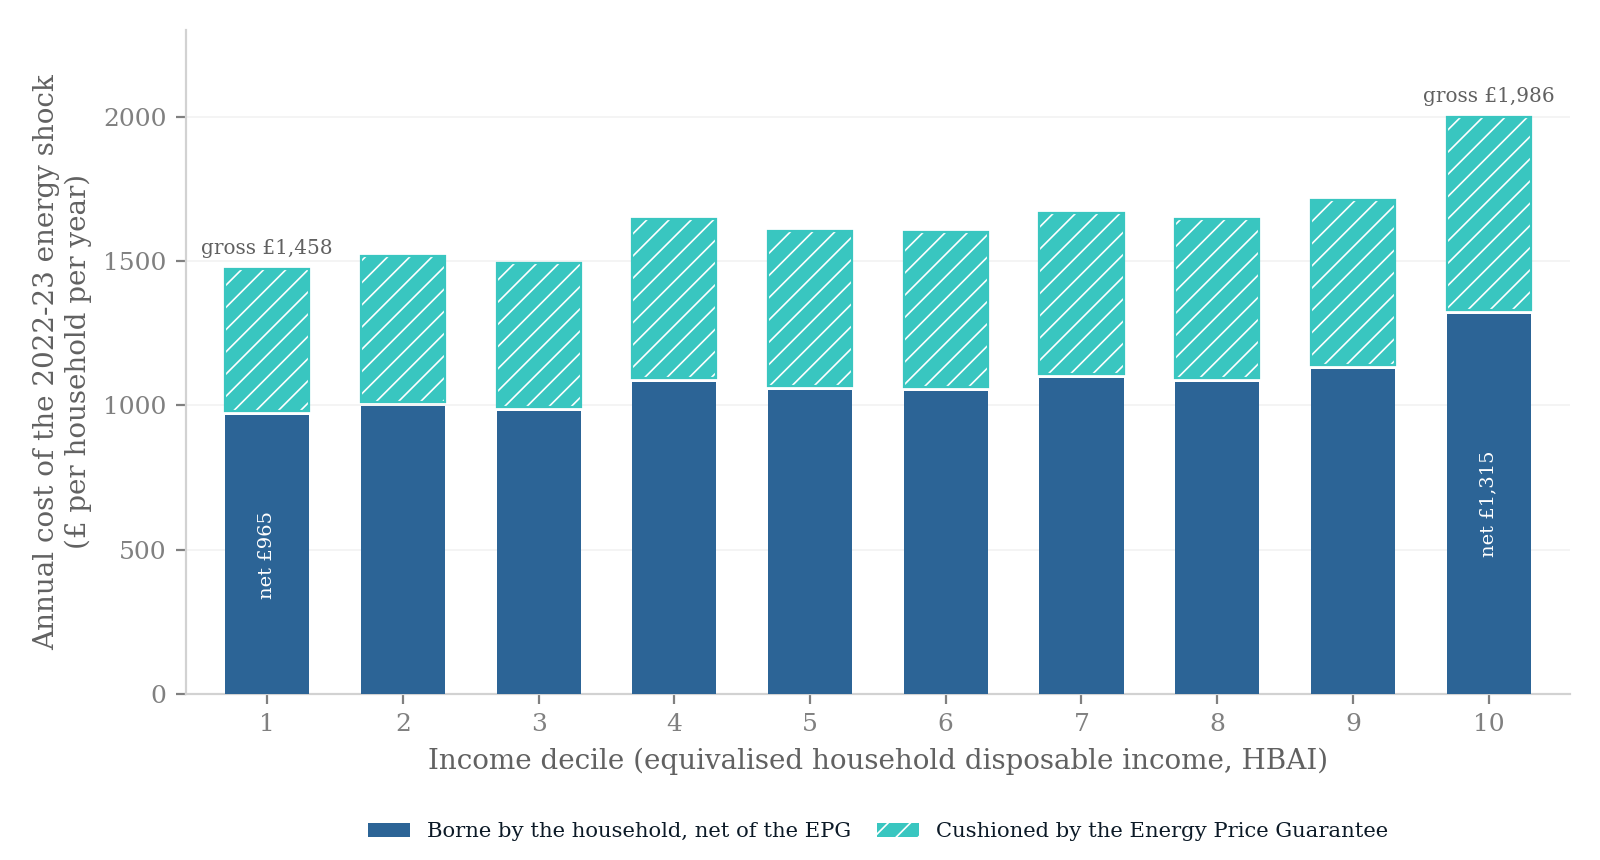
\includegraphics[width=\textwidth]{figures/fig_energy_epg.png}
\caption{Energy shock by decile: the part households bore net of the Energy Price Guarantee and the part it absorbed (a constant \MsEnergyCushionShareFyPct\ per cent; \pounds\MsEnergyCushionGbpDecOne\ to \pounds\MsEnergyCushionGbpDecTen\ a year).}
\label{fig:energy-epg}
\end{figure}

\subsection{Household-stage conventions in full}\label{app:conventions}

\runin{Exposure variable.} The household energy exposure is
the model's domestic energy consumption, with a weighted mean of
\pounds 1{,}632 at 2024--25 prices. In this dataset domestic energy is
exactly electricity plus gas, so no off-grid fuel spending is treated
as capped. The mean divides out of every aggregate through the rebase,
so the headline levels do not depend on it.

\runin{Coverage.} The Energy Price Guarantee enters as the difference
between the two capped paths, the Energy Bills Support Scheme as its
flat \pounds 400 to every weighted household (the modelled
\pounds\SsEbssBn\ billion compares with a \pounds\SsEbssOutturnBn\
billion NAO outturn; the model applies no supply screen, and the
scheme paid per electricity meter, second homes included), and the
2022--23
cost-of-living payments on PolicyEngine UK's own 2022--23 eligibility
rules (the means-tested payment per benefit unit, the pensioner
payment through Winter Fuel Payment eligibility, and \pounds 150 per
disabled person), \pounds\SsColBn\ billion in total; modelled
eligibility in the simulated year is not receipt in the actual 2022
qualifying windows.

The
council-tax rebate and the Warm Home Discount are not modelled. The
discretionary total is therefore an approximation with omissions on
both sides, not a bound.

\runin{Weights.} The person
weights gross to \SsPersonsM\ million people, in line with the UK
population. The household grossing weights total
\SsWeightedHouseholdsM\ million households against an ONS count of
\SsOnsHouseholdsM\ million, so aggregates sit about \SsWeightExcessPct\ per cent above an ONS-count basis; ratios are unaffected.

Deciles are
equivalised on the Households Below Average Income (HBAI)
before-housing-costs concept, and burdens are
expressed as shares of household expenditure rather than income,
because a ratio with income in the denominator is dominated by
very low incomes. Both sides of every share sit on one base: the burden numerator is
rebased to FY2021--22 cap levels, and the expenditure denominator to
the ONS FYE2022 mean total-spending base the decile-table analysis divides by
(factor \SsSpendRebase), so household-stage shares are level-comparable
with the decile-table analysis. The rebase factors are common scalars, so the variance decomposition
and all quantile ratios are invariant to them (the within-share is
\SsWithinPct\ per cent on either base). Aggregate pounds are reconciled in Appendix~\ref{app:recon}.

\runin{Deflated inputs.} The households carry 2024--25 nominal
incomes. Deflating \SsDeflInputsScaled\ monetary inputs to 2023--24 by
the model's own uprating indices (earnings by
\SsDeflEarningsFactorTwentyThreePct\ per cent) gives a full-stack rate
of \SsDeflFullRatePct\ per cent (\SsDeflFullRateDiffPp\ points) and
moves no decile by more than \SsDeflMaxDecileDiffPp\ points; deflating
to 2022--23 (earnings by \SsDeflEarningsFactorTwentyTwoPct\ per cent)
under 2022--23 rules gives \SsDeflRulesTwentyTwoFullRatePct\ per cent.
Weights are not rescaled.

\subsection{The tariff earnings scenario}\label{app:e3}

The shock to division $j$ is $s_j=\tau_j x_j \varepsilon \pi$: the
tariff rate $\tau_j$, the US-export share of turnover $x_j$ (HMRC
trade by industry over ONS Annual Business Survey turnover, for 23 SIC
divisions), an export-demand elasticity $\varepsilon$ and the
wage-bill incidence $\pi$. Both $\varepsilon$ and $\pi$ are set to one
as a unit stress. The scenario omits price changes, imported inputs,
profits and general-equilibrium effects, and the sector weights are
an accounting bridge, not measured tariff incidence.

Two margins deliver the same gross loss,
\pounds\EThreeDispGrossM\ million. Under the wage cut,
every employee in division $j$ loses the share $s_j$ of earnings, with
pension contributions scaled. Under displacement, each employee loses
the job for the full year with probability $s_j$, independently:
status becomes unemployed, and earnings, hours, pension contributions
and statutory pay are set to zero.

Baseline and shocked systems are run under 2026--27 rules on the
Microcosm UK records, projected forward from 2024--25 to 2026--27 with
the model's own uprating indices (incomes and weights). The cushioning rate is one minus the fall in
HBAI household net income over the fall in gross employee earnings.
The displacement rate is the exact expectation over the independent
job-loss draws, computed from all \EThreeDispExposedRecords\ exposed
records in \EThreeDispExposedHouseholds\ households (about
\EThreeDispExactEffRecords\ effective; the largest record carries
\EThreeDispExactMaxShare\ per cent of the loss). It has no Monte Carlo
error; its standard error of \EThreeDispSamplingSe\ points is survey
sampling error, clustered on households. Benefit units newly entitled
to Universal Credit claim with an assumed probability of 0.8 (no
official Universal Credit take-up estimate exists), mixed exactly in
the expectation; others keep their baseline flags, and baseline
poverty lines are frozen. The wage-cut rate averages \EThreeWageDraws\
take-up draws.

Displaced workers receive an approximation of contribution-based New
Style Jobseeker's Allowance: \EThreeDispJsaWeeks\ weeks at the model's
rates for those unemployed, aged 18 to state pension age, with
baseline earnings of at least 50 times the weekly lower earnings
limit, with no partner test and full take-up. It is an upper bound,
since waiting days, pension abatement and sanctions are omitted. It
pays \pounds\EThreeDispJsaPaidM\ million, lowers Universal Credit by
\pounds\EThreeDispJsaUcOffsetM\ million and adds
\EThreeDispJsaEffectPts\ points: without it the displacement rate is
\EThreeDispNoJsaRatePct\ per cent.

Table~\ref{tab:e3-split} splits the cushion. Income tax accounts for
the gap between the margins; Universal Credit and the New Style
allowance narrow it. The pension row is employee contributions
ceasing, which HBAI income deducts, not tax or benefit. The model
holds reported student-loan repayments fixed, so the cushion is
slightly understated.

\begin{table}[tbp]
\centering
\caption{Tariff scenario: cushioning by component, per cent of the gross earnings loss}
\label{tab:e3-split}
\small
\begin{tabular}{lrrr}
\toprule
 & Wage cut & Displacement & Displacement, \\
 & & & no New Style JSA \\
\midrule
Income tax & \EThreeWageTaxOfGrossPct & \EThreeDispTaxOfGrossPct & \EThreeDispNoJsaTaxOfGrossPct \\
National Insurance & \EThreeWageNiOfGrossPct & \EThreeDispNiOfGrossPct & \EThreeDispNoJsaNiOfGrossPct \\
Universal Credit & \EThreeWageUcOfGrossPct & \EThreeDispUcOfGrossPct & \EThreeDispNoJsaUcOfGrossPct \\
New Style Jobseeker's Allowance & \EThreeWageJsaContribOfGrossPct & \EThreeDispJsaContribOfGrossPct & \EThreeDispNoJsaJsaContribOfGrossPct \\
Pension contributions & \EThreeWagePensionOfGrossPct & \EThreeDispPensionOfGrossPct & \EThreeDispNoJsaPensionOfGrossPct \\
\midrule
Cushioning rate & \EThreeWageRatePct & \EThreeDispRatePct & \EThreeDispNoJsaRatePct \\
\bottomrule
\end{tabular}
\begin{minipage}{.85\textwidth}\footnotesize
\emph{Notes:} Rows omit small items (other benefits, child benefit,
statutory pay, the floor on negative incomes), so they do not sum
exactly to the rate. Taxes and benefits alone, net of the pension row,
offset \EThreeWageTaxBenRatePct\ (wage cut) and
\EThreeDispTaxBenRatePct\ (displacement) per cent.
\end{minipage}
\end{table}

Redundancy pay, partial-year spells, re-employment and behavioural
responses are not modelled. The Exchequer cost is
\pounds\EThreeWageExchequerM\ million (wage cut) and
\pounds\EThreeDispExchequerM\ million (displacement), above the
household-side offset because the government balance includes
employer contributions. Poverty before housing costs rises
\EThreeDispPovertyPp\ points under displacement. By decile of
equivalised HBAI income (person-weighted, unlike the household deciles
of the price episodes), the loss per person a year from bottom to top
is \pounds\EThreeDispDecGbpOne, \EThreeDispDecGbpTwo,
\EThreeDispDecGbpThree, \EThreeDispDecGbpFour, \EThreeDispDecGbpFive,
\EThreeDispDecGbpSix, \EThreeDispDecGbpSeven, \EThreeDispDecGbpEight,
\EThreeDispDecGbpNine\ and \EThreeDispDecGbpTen\ under displacement
and \pounds\EThreeWageDecGbpOne, \EThreeWageDecGbpTwo,
\EThreeWageDecGbpThree, \EThreeWageDecGbpFour, \EThreeWageDecGbpFive,
\EThreeWageDecGbpSix, \EThreeWageDecGbpSeven, \EThreeWageDecGbpEight,
\EThreeWageDecGbpNine\ and \EThreeWageDecGbpTen\ under wage cuts. At the OBR's
elasticity of 0.4 the gross loss is \pounds\EThreeObrLowWageGrossM\
million and the wage-cut rate \EThreeObrLowWageRatePct\ per cent; the
displacement rate is unchanged by construction, because the
expectation reweights the same job-loss passes. A Monte Carlo
check with \EThreeBernDraws\ Bernoulli assignment draws and no New Style
allowance gives a pooled rate of \EThreeBernRatePooled\ per cent
(standard error \EThreeBernRatePooledSe; per-draw mean
\EThreeBernRateMean, range
\EThreeDispRateMin--\EThreeDispRateMax), close to the
exact rate without the allowance (\EThreeDispNoJsaRatePct\ per cent).

\subsection{The model's native instruments and the decile ranking}\label{app:native}

The model does
contain one entitlement that reads energy consumption: PolicyEngine
UK's own Energy Price Guarantee variable, which pays
\pounds\SsNativeEpgBn\ billion in the 2023 baseline and rises by
\pounds\SsNativeEpgDeltaBn\ billion under the shocked inputs, moving
household benefits by the same amount. That delta verifies that the variable responds. It is measured around
the dataset's current-vintage energy levels, with shocked inputs above the unrebased baseline, so it is not
comparable to the \pounds\SsEpgBn\ billion cushion, which is defined
against the FY2021--22 base.

The paper classifies the
Guarantee as discretionary and models it on the financial-year basis
of Section~\ref{sec:secondstage-method} rather than through the
model's calendar-year variable; the model's cost-of-living payment
variable (\pounds\SsNativeColBn\ billion at 2023--24 amounts) sits
inside the HBAI income that ranks the deciles, as do the native
Guarantee (\pounds\SsNativeEpgBn\ billion) and the
\pounds\SsNativeEbrBn\ billion energy-bills rebate, so the deciles
are ranked on income inclusive of these 2023 support instruments. The cushioning arithmetic itself counts each
separately modelled instrument once, and the ranking is not driving the
gradient: re-ranking deciles on income net of the three native
instruments moves the bottom decile's full-stack rate from
\SsRankBaseDOne\ to \SsRankNetDOne\ per cent and the top decile's
from \SsRankBaseDTen\ to \SsRankNetDTen, so the rates-fall-with-income
result survives.

\subsection{Reconciliations}\label{app:recon}

\paragraph{Energy budget shares.} One comparator needs reconciling. \citet{rf2022} report energy budget
shares of roughly 11 per cent in the second decile against 6 per cent
in the ninth; the shares computed here are
\MsEnergyBudgetSharePctDecTwo\ and
\MsEnergyBudgetSharePctDecNine\ per cent. The gap is definitional,
not substantive: this paper measures electricity and gas only, as a
share of \emph{total spending}, on equivalised-income deciles of the
FYE2022 vintage, whereas the wider comparator includes other domestic
fuels and is expressed against income. Because the episode's incidence
is linear in this share, the difference scales the level of every
energy number reported here, another reason to prefer the household stage, which computes the share directly rather than importing it.

\paragraph{Household-stage and decile-table aggregates.} On the same
financial-year basis the decile-table analysis puts the counterfactual
shock at \pounds\MsEnergyGrossAggBn\ billion and the realised path at
\pounds\MsEnergyRealisedAggBn\ billion, against
\pounds\SsCounterAggBn\ and \pounds\SsRealisedAggBn\ billion on
household records. Two known offsets separate them: the grossing
weights, \SsWeightExcessPct\ per cent above the ONS household count,
and the rebase convention, which sets the weighted mean bill to the
FY2021--22 cap mean rather than to the ONS FYE2022 mean spend. Ratios
are unaffected; levels should be read with the gap in mind.

\subsection{Universal Credit uprating arithmetic for a single adult}\label{sec:results-rulebook}

Two statutory facts frame the crisis year. First, the
uprating lag: Universal Credit's standard allowance rose 3.1 per cent
in April 2022 (indexed to the previous September's inflation) while
prices rose at double digits. Against month-by-month contemporaneous
indexation (an upper-bound counterfactual under which no actual
benefit system operates), a single adult's standard allowance fell
\pounds\MsUcLagCostGbp\ short over 2022--23
(\MsUcLagCostPctAllowance\ per cent of the annual allowance); against
the alternative of a single April 2022 uprating at
contemporaneous annual CPI, \pounds\MsUcLagCostFlatAltGbp. Both
figures are for the single-adult standard allowance only, before
elements and caseload weighting; the range, not either point, is the result.

Neither the lag nor its cost is a discovery of this
paper: \citet{cribb2023} quantified the 2022--23 shortfall and scored
the discretionary cost-of-living payments against a timely-indexation
counterfactual, and \citet{obrwelfare2022} put the aggregate real fall
at roughly \pounds 12 billion, a figure the household stage's
\pounds\SsLagReformBn\ billion (Section~\ref{sec:results-indexation})
does not reproduce: the bases and price counterfactuals differ, and the two
are stated side by side rather than reconciled. This paper's addition is the
join: the lag priced against trade-shock incidence, on the same
households, across episodes.

The 2022--23 shortfall was a timing loss later reversed in the level
of awards, though not repaid; below-inflation uprating in other years
reflected freezes and caps \citep{judgemurphy2023}. The shortfall
arises from timing, and it coincides with the period in which the
terms-of-trade shock peaked. Figure~\ref{fig:uprating-lag} shows the gap month by month. Second,
sequencing: the \pounds\MsUcUpliftRemovalGbp-a-year
Covid uplift was removed in October 2021, months before the energy
shock landed, so the uplift's end preceded the largest price-led trade
shock of the period.

Together
with the Guarantee's absorption of \MsEnergyCushionShareFyPct\ per cent of the
counterfactual shock, the picture is: an automatic response on the
earnings margin (in the tariff scenario), a discretionary
response on the price margin, and indexation that followed prices with
a year's lag, with the incidence of the full discretionary stack reported in Section~\ref{sec:results-secondstage}.

\begin{figure}[tbp]\centering
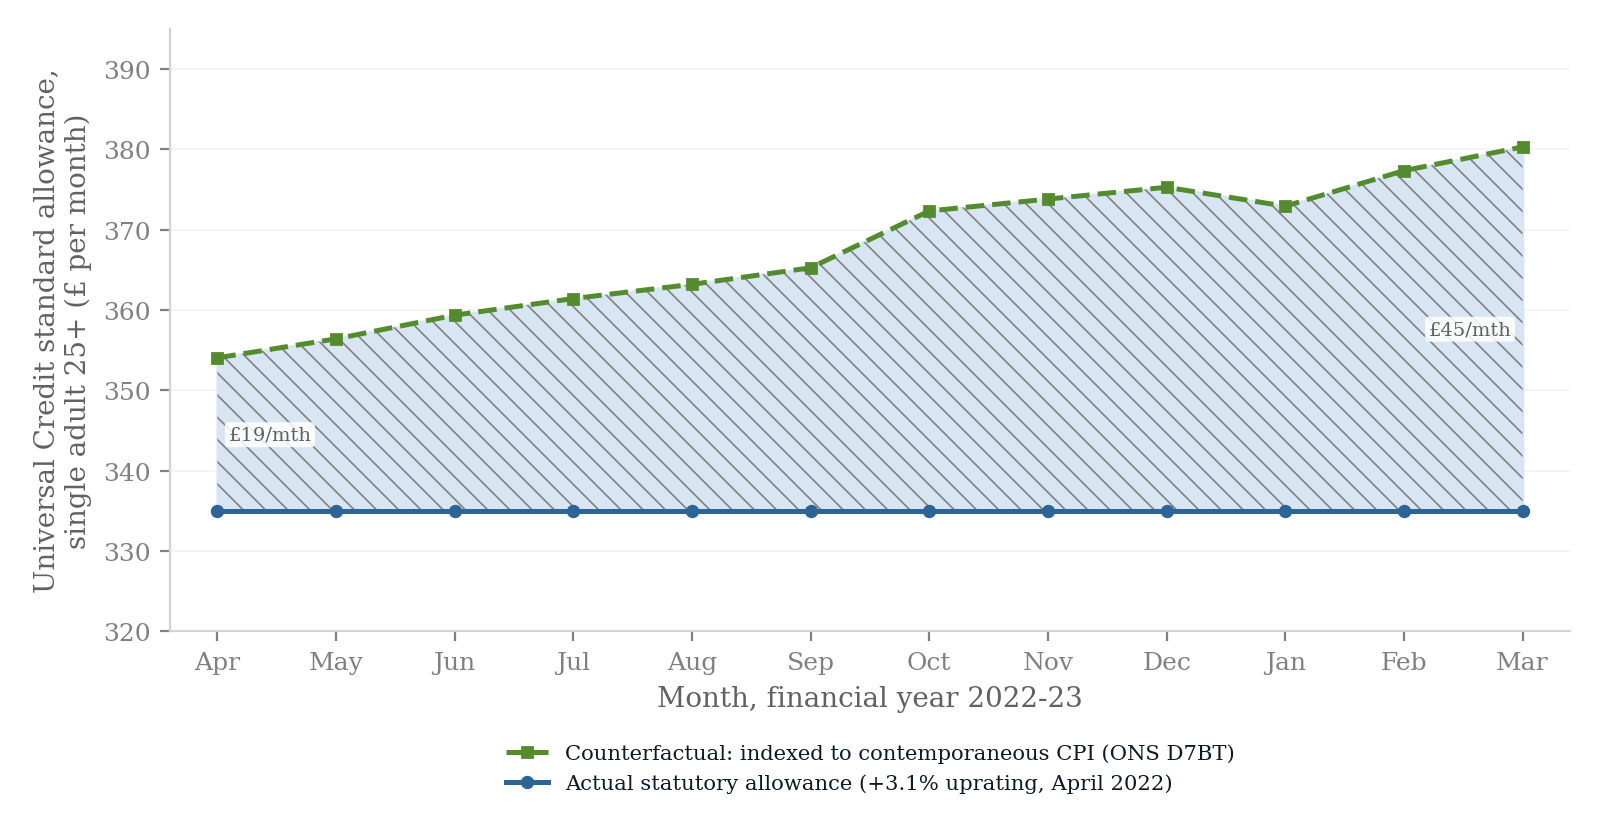
\includegraphics[width=\textwidth]{figures/fig_uprating_lag.png}
\caption{Universal Credit standard allowance, single adult 25+, against a contemporaneous-CPI counterfactual. The shaded shortfall sums to \pounds\MsUcLagCostGbp\ over 2022--23.}
\label{fig:uprating-lag}
\end{figure}

\subsection{The two-axis sensitivity grid}\label{sec:results-grid}

Table~\ref{tab:grid} and Figure~\ref{fig:grid} vary the two conventions the headline rates
depend on: the rebase factor (the paper's computed \SsRebaseFactor,
an intermediate 0.8, and 1.0, no rebase) and the discretionary stack,
built up one instrument at a time. First, the Guarantee's cushioning rate
(\SsGridPaperEpgRatePct\ per cent) is invariant to \emph{both}
axes, to the rebase because a price cap scales with the bill it
truncates, and across deciles by the accounting identity already
noted, so every pound of progressivity and every point of
rebase-sensitivity in the headline comes from the flat-cash
instruments.

Second, across the grid the full
stack cushions \SsGridPaperFullRatePct\ per cent of the
counterfactual shock at the paper's rebase and
\SsGridUnityFullRatePct\ per cent with no rebase at all, and the
progressive gradient survives every cell: without rebasing, the full
stack returns \SsGridUnityFullDOne\ per cent of the bottom
decile's loss against \SsGridUnityFullDTen\ per cent of the top
decile's. The direction of the results holds across the grid, and
no decile's point estimate exceeds 100 per cent at rebase factors of \SsRebaseFactor\ or above (the third decile's is highest, at \SsCushionPctDecThree; Figure~\ref{fig:grid} extends the aggregate rate to lower factors): the bottom
decile's is \SsGridPaperFullDOne\ per cent at the paper's rebase and
\SsGridUnityFullDOne\ per cent without rebasing.

One external anchor bears on the
choice of cell: at a
rebase of one the Guarantee's absorption is \pounds\SsEpgBn\ billion divided
by the rebase factor \SsRebaseFactor, about \pounds 20 billion, closer to the NAO's \pounds 24.0 billion outturn \citep{nao2024}, while the paper's
rebase gives \pounds\SsEpgBn\ billion. Any match is partly
coincidental, the outturn reflects the actual caps, a longer window
and price-dependent
volumes, but it cautions against reading the rebased cell as the
truth and the unrebased one as a variant. The paper's headline
statements are therefore confined to what holds across the grid.

The counterfactual \emph{path} is also varied: carrying the October 2022 cap through the second half-year is a convention, not a forecast,
so the grid is complemented by a variant using the January 2023 cap that Ofgem actually set (\pounds 4{,}279) for the final quarter, giving an FY mean of \pounds\SsAnnCounterFyCap\
and a counterfactual shock of \pounds\SsAnnCounterAggBn\ billion. On
that path the Guarantee absorbs \SsAnnEpgRatePct\ per cent and the
full stack \SsAnnFullRatePct\ per cent: the paper's two-cap convention gives the lower rate on the path axis and the energy-specific
attribution the lower rate on the attribution axis; neither is a
bound, because the rebase axis is a convention rather than an
estimate.

Seasonality is varied the same way. The model's monthly profile puts
\SsSeasShareAprSepPct\ per cent of energy consumption in
April--September, \SsSeasShareOctDecPct\ in October--December and
\SsSeasShareJanMarPct\ in January--March. The Guarantee absorbs
\pounds\SsSeasEqHeldEpgBn\ billion on the headline convention (equal
half-year weights, October cap held), \pounds\SsSeasEqActualEpgBn\
billion with the actual caps and \pounds\SsSeasCwActualEpgBn\ billion
with the actual caps and consumption weights, against an outturn of
\pounds 24.0 billion \citep{nao2024}: the last two bracket the
outturn. The full-stack rate is \SsSeasEqHeldFullRatePct,
\SsSeasEqActualFullRatePct\ and \SsSeasCwActualFullRatePct\ per cent,
so the headline is the conservative case.

\begin{table}[tbp]
\centering
\caption{Cushioning under two conventions: rebase factor $\times$
discretionary stack}
\label{tab:grid}
\small
% generated by grid_energy.py -- do not edit by hand.
\begin{tabular}{llrrrr}
\toprule
Rebase & Stack & Shock (\pounds bn) & Rate (\%) & D1 (\%) & D10 (\%) \\
\midrule
0.740 (paper) & None & 45.0 & 0.0 & 0.0 & 0.0 \\
 & EPG only & 45.0 & 33.8 & 33.8 & 33.8 \\
 & EPG + EBSS & 45.0 & 59.5 & 62.5 & 54.0 \\
 & Full stack & 45.0 & 79.9 & 93.6 & 58.7 \\
\addlinespace
0.800 & None & 48.6 & 0.0 & 0.0 & 0.0 \\
 & EPG only & 48.6 & 33.8 & 33.8 & 33.8 \\
 & EPG + EBSS & 48.6 & 57.6 & 60.3 & 52.5 \\
 & Full stack & 48.6 & 76.5 & 89.1 & 56.8 \\
\addlinespace
1.000 & None & 60.8 & 0.0 & 0.0 & 0.0 \\
 & EPG only & 60.8 & 33.8 & 33.8 & 33.8 \\
 & EPG + EBSS & 60.8 & 52.9 & 55.0 & 48.7 \\
 & Full stack & 60.8 & 67.9 & 78.0 & 52.2 \\
\bottomrule
\end{tabular}

\begin{minipage}{.85\textwidth}\footnotesize
\emph{Notes:} Each cell is arithmetic on the same simulated
households; the measured automatic response is zero in every cell
(Section~\ref{sec:results-secondstage}), so no re-simulation is
required. ``Rate'' is the discretionary cushioning rate against the
counterfactual shock on the financial-year basis; D1 and D10 are the
bottom- and top-decile rates. The EPG row's rate is constant across
rebase and deciles by construction.
\end{minipage}
\end{table}

\begin{figure}[tbp]\centering
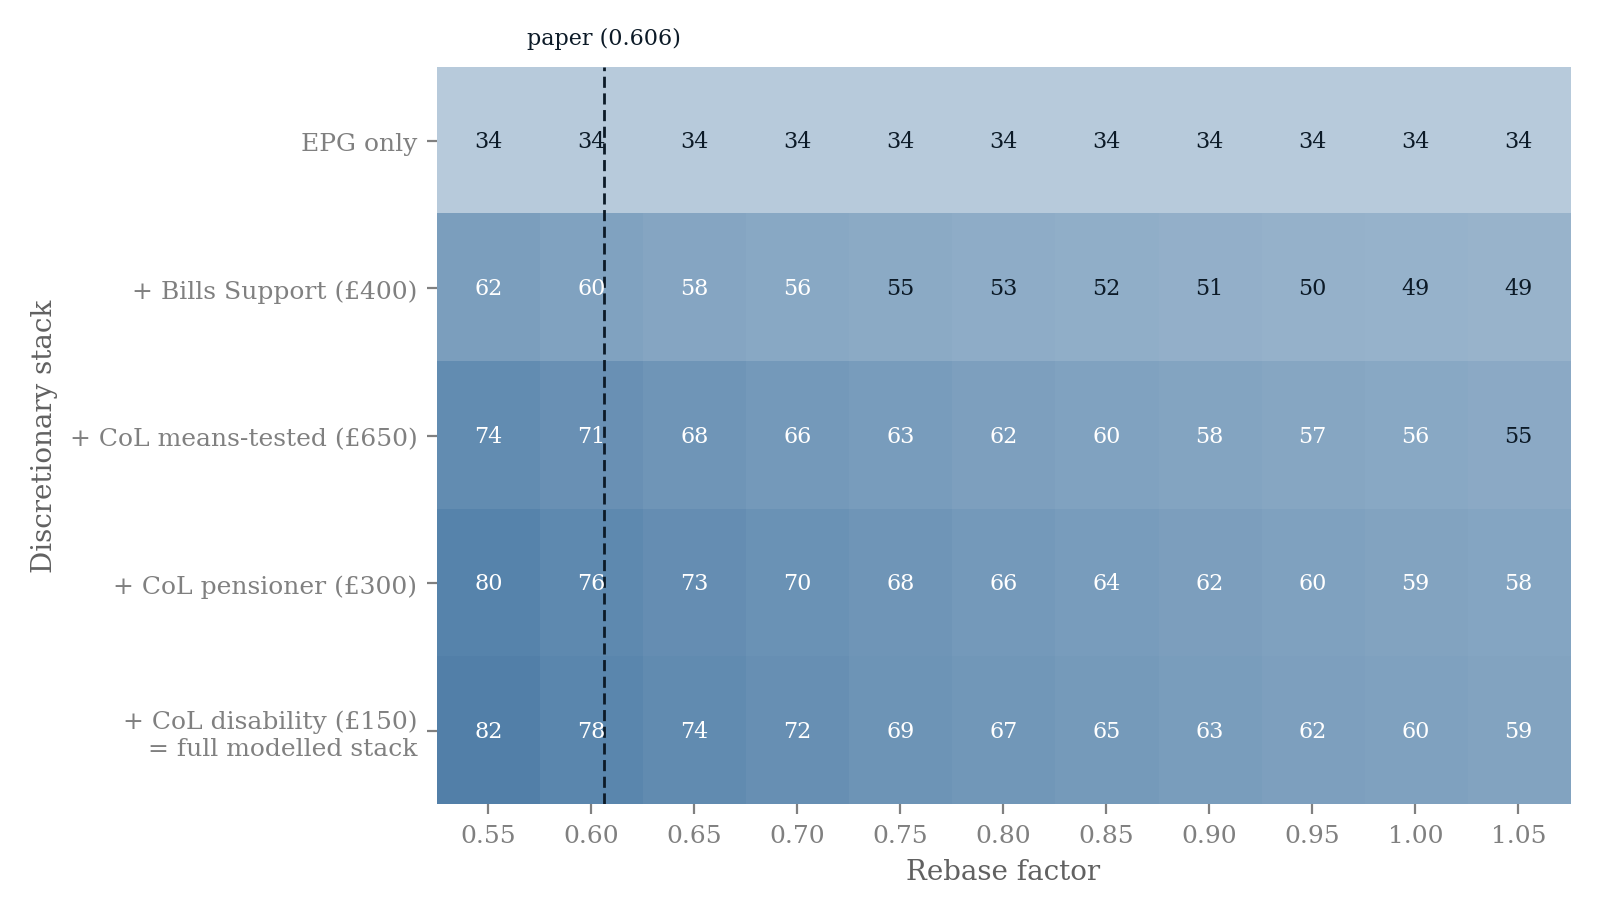
\includegraphics[width=\textwidth]{figures/fig_grid.png}
\caption{Discretionary cushioning rate by rebase factor (0.55--1.05) and instrument stack. Dashed rule: the paper's rebase. The EPG row is constant; all variation comes from the flat-cash payments.}
\label{fig:grid}
\end{figure}

\begin{figure}[tbp]\centering
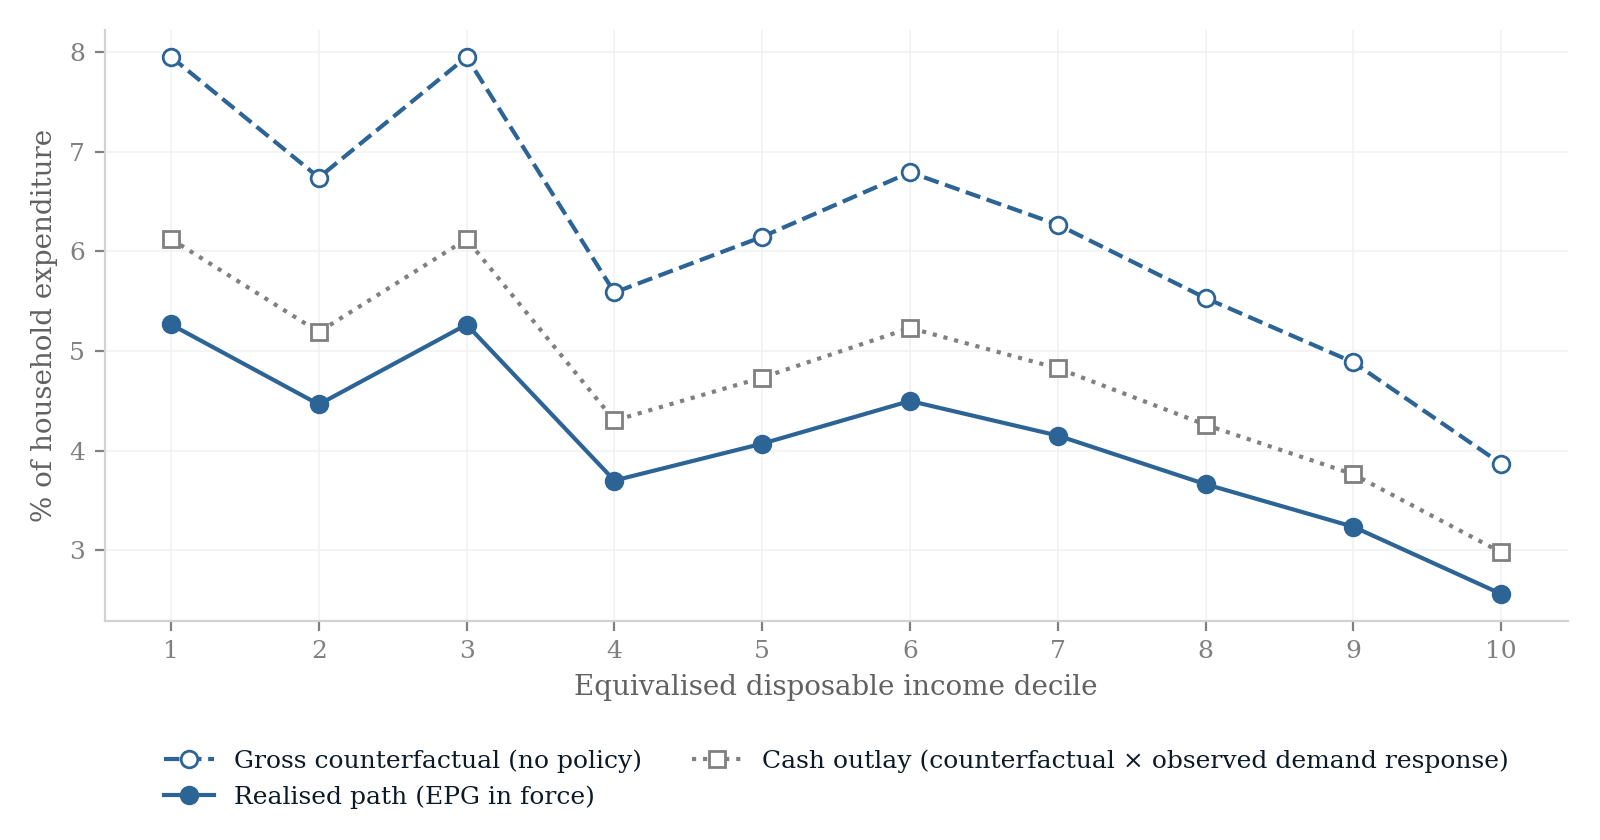
\includegraphics[width=\textwidth]{figures/fig_paths.png}
\caption{Energy burden as a share of spending by decile under three paths: no policy, Energy Price Guarantee in force (realised), and cash outlay, the realised path scaled by the observed demand response.}
\label{fig:paths}
\end{figure}

\subsection{From incidence to demand and welfare}\label{sec:results-mpc}

The statutory incidence measured above is an accounting object. This
subsection aggregates it into two economic ones, keeping the paper's
conventions: every behavioural parameter is imported from the
literature and stated, nothing is estimated, and the outputs are
first-round policy-simulation quantities, no general-equilibrium
feedback, no intertemporal response.

\runin{Demand.} Each flow of the energy episode, the counterfactual
burden and the three instruments, is weighted by a marginal
propensity to consume assigned by equivalised-income decile, under
three assumed scenarios: a gradient falling from 0.8 in the bottom
decile to 0.3 in the top, a deliberately steep stylisation of the
cash-on-hand and liquidity gradients of \citet{jappelli2014} and
\citet{fagereng2021}, whose mapping into income deciles is flatter; a flat 0.5, which
switches the heterogeneity channel off; and an asymmetric UK variant
after \citet{bunn2018}, who find MPCs out of income \emph{losses}
far larger than out of gains; the variant assumes 0.5 and 0.14.

Table~\ref{tab:mpc} reports the results, with the flat scenario as
the anchor and the gradient as the deliberately steep variant. First,
under the gradient the counterfactual shock corresponds to a
first-round consumption fall of \pounds\SsMpcBurdenGradientBn\
billion (\pounds\SsMpcBurdenFlatBn\ billion on the flat anchor); with
the full stack the net first-round effect is
$\SsMpcNetGradientBn$ billion pounds.

Second, under the gradient
scenario only, first-round consumption per pound of modelled outlay is
\SsMpcColPerPound\ for the cost-of-living payments,
\SsMpcEbssPerPound\ for the Energy Bills Support Scheme and
\SsMpcEpgPerPound\ for the Guarantee; under the flat and asymmetric
scenarios the three coincide, so the ordering is a property of the
assumed gradient rather than an estimated one. Third, the asymmetric
scenario applies the assumed gain-MPC of 0.14 to every
instrument, although the Guarantee truncates a loss rather than paying
a windfall; taken at face value the net first-round demand effect is
$\SsMpcNetAsymBn$ billion pounds.

\runin{Welfare.} Weighting the counterfactual burden by
\citet{atkinson1970} welfare weights proportional to $y^{-\gamma}$ and
normalised to mean one, the simplest case of the generalised welfare
weights of \citet{saezstantcheva2016}, with equivalised income $y$
floored at \pounds 1{,}000 a year (an assumption to which the
$\gamma=2$ premium is sensitive), gives a regressivity premium, the
ratio of the welfare-weighted burden to that of an equal-pounds
shock of the same total, of \SsWelfPremiumGammaOne\ at $\gamma=1$ and
\SsWelfPremiumGammaTwo\ at $\gamma=2$. Both are below one: the shock is
regressive in \emph{shares} but larger in \emph{pounds} at the top, so
inequality-averse weights on pounds do not amplify its welfare cost
relative to an equal-pounds shock, at either value of $\gamma$.

\begin{table}[tbp]
\centering
\caption{First-round demand effects of the energy episode under
assumed MPC scenarios}
\label{tab:mpc}
\small
% generated by mpc_welfare.py -- do not edit by hand.
\begin{tabular}{lrrr}
\toprule
 & \multicolumn{3}{c}{First-round demand effect, \pounds bn}\\
\cmidrule(lr){2-4}
Flow & MPC gradient & MPC flat & Fiscal flow \\
\midrule
Counterfactual burden (no policy) & $-$24.1 & $-$22.5 & $-$45.0 \\
Energy Price Guarantee & 8.1 & 7.6 & 15.2 \\
Bills Support Scheme & 6.4 & 5.8 & 11.6 \\
Council Tax energy rebate & 1.9 & 1.7 & 3.4 \\
Cost-of-living payments & 5.7 & 4.6 & 9.2 \\
Net position (full stack) & $-$2.0 & $-$2.8 & $-$5.7 \\
\bottomrule
\end{tabular}

\begin{minipage}{.85\textwidth}\footnotesize
\emph{Notes:} MPC gradient: 0.8 (bottom decile) to 0.3 (top),
linear; MPC flat: 0.5 everywhere. The asymmetric variant
(after \citealp{bunn2018}; assumed 0.5 out of losses, 0.14 out of gains) gives a
net effect of $\SsMpcNetAsymBn$ billion pounds (not shown by row).
First-round, no general-equilibrium feedback; parameters imported,
not estimated. Rates and sums are computed on unrounded arrays, so
displayed rows may differ from column sums in the last digit.
\end{minipage}
\end{table}


\end{document}
